\documentclass[12pt,a4paper]{article}

% Package for setting margins
\usepackage[left=2.5cm, right=2.5cm, top=2.5cm, bottom=2.5cm]{geometry}

\usepackage[T1]{fontenc}
\usepackage{ebgaramond}
\usepackage{libertinus}

% Set 1.5 line spacing
\usepackage{setspace}
\onehalfspacing

% Full justification (default in LaTeX)
% Package for better justification
\usepackage{ragged2e}

% Enable page numbers
\pagestyle{plain}

% Other useful packages
\usepackage{graphicx}
\usepackage{hyperref}
\usepackage{xcolor}
\usepackage[final]{microtype}
\emergencystretch=2em

% Custom added
\usepackage{amsmath}
\usepackage{float}

\definecolor{titleaccent}{RGB}{0,84,136}

\newcommand{\titlepagelogo}[1]{%
    \IfFileExists{#1}{%
        \includegraphics[height=1.9cm]{#1}%
    }{%
        \fbox{\parbox[c][1.9cm][c]{3.2cm}{\centering\footnotesize Logo\\placeholder}}%
    }%
}

\newcommand{\titlepagefont}{\ebgaramond}

\begin{document}

% Title page
\begin{titlepage}
    \thispagestyle{empty}
    \noindent
    \begin{minipage}[c]{0.28\textwidth}
        \raggedright
        \titlepagelogo{logos/university.png}
    \end{minipage}%
    \hspace*{0.14\textwidth}%
    \begin{minipage}[c]{0.24\textwidth}
        \centering
        \titlepagelogo{logos/faculty.png}
    \end{minipage}%
    \hspace*{0.10\textwidth}%
    \begin{minipage}[c]{0.24\textwidth}
        \raggedleft
        \titlepagelogo{logos/chair.png}
    \end{minipage}

    \vspace*{2.3cm}

    \centering
    {\color{titleaccent}\rule{0.72\textwidth}{1.2pt}\par}
    \vspace{0.9cm}
    {{\titlepagefont\fontsize{26}{31}\selectfont\scshape The Unreasonable Effectiveness of Data for Recommender Systems\par}}
    \vspace{0.9cm}
    {{\titlepagefont\Large Master's Thesis\par}}
    \vspace{0.25cm}
    {{\titlepagefont\large in Computer Science\par}}
    \vspace{0.9cm}
    {\color{titleaccent}\rule{0.48\textwidth}{0.8pt}\par}

    \vspace{1.5cm}
    {{\titlepagefont\Large Youssef Abdou\par}}
    \vspace{0.35cm}
    {{\titlepagefont\large University of Siegen\par}}
    \vspace{0.15cm}
    {{\titlepagefont\large \today\par}}

    \vfill

    \noindent
    \hfill
    \begin{minipage}[t]{0.5\textwidth}
        \raggedleft
        {\titlepagefont\large ISG: Intelligent Systems Group\par}
        \vspace{0.7cm}
        {\titlepagefont\large\bfseries Examiners\par}
        \vspace{0.2cm}
        {\titlepagefont Prof. Dr.-Ing Jöran Beel\par}
        {\titlepagefont M. Sc. Tobias Vente\par}
        \vspace{0.25cm}
        {\titlepagefont\rule{0.85\linewidth}{0.4pt}\par}
    \end{minipage}
\end{titlepage}

% Formal submission page
\begin{titlepage}
    \thispagestyle{empty}
    \titlepagefont
    \vspace*{\fill}

    \noindent
    This Master's Thesis is handed in according to the requirements of the University of Siegen for the study program Master Computer Science of the year 2021 (PO 2021).

    \vspace{1.6cm}

    \noindent{\large\bfseries Process period\par}
    \vspace{0.2cm}
    22.09.2025 to 23.03.2026

    \vspace{1.0cm}

    \noindent{\large\bfseries Examiners\par}
    \vspace{0.2cm}
    Prof. Dr.-Ing.\ J\"oran Beel\par
    M. Sc. Tobias Vente

    \vspace*{\fill}
\end{titlepage}

% Declaration of authorship page
\begin{titlepage}
    \thispagestyle{empty}
    \titlepagefont
    \vspace*{\fill}

    \noindent{\Large\bfseries Eigenst\"andigkeitserkl\"arung\par}

    \vspace{0.8cm}

    \noindent
    Ich versichere, dass ich die schriftliche Ausarbeitung selbst\"andig angefertigt und keine anderen als die angegebenen Hilfsmittel benutzt habe. Alle Stellen, die dem Wortlaut oder dem Sinn nach (inkl. \"Ubersetzungen) anderen Werken entnommen sind, habe ich in jedem einzelnen Fall unter genauer Angabe der Quelle (einschlie\ss lich des World Wide Web sowie generativer KI und anderer elektronischer Datensammlungen) deutlich als Entlehnung kenntlich gemacht. Dies gilt auch f\"ur angef\"ugte Zeichnungen, bildliche Darstellungen, Skizzen und dergleichen. Ich nehme zur Kenntnis, dass die nachgewiesene Unterlassung der Herkunftsangabe als versuchte T\"auschung gewertet wird.

    \vspace{0.8cm}

    \noindent
    Ich best\"atige, dass die elektronische Version inhaltlich mit der gedruckten Version \"ubereinstimmt.

    \vspace{1.8cm}

    \noindent
    \begin{minipage}[t]{0.45\textwidth}
        \raggedright
        \rule{0.9\linewidth}{0.4pt}\par
        Datum
    \end{minipage}%
    \hfill
    \begin{minipage}[t]{0.45\textwidth}
        \raggedright
        \rule{0.9\linewidth}{0.4pt}\par
        Unterschrift
    \end{minipage}

    \vspace{1.6cm}

    \noindent{\Large\bfseries Declaration of Authorship\par}

    \vspace{0.8cm}

    \noindent
    I certify that I have prepared this written work independently and have not used any aids other than those specified. I have clearly identified all passages that are taken from other works in terms of wording or meaning (including translations) as borrowed material in each individual case, stating the exact source (including the World Wide Web as well as generative AI and other electronic data collections). This also applies to attached drawings, pictorial representations, sketches and the like. I acknowledge that the proven omission of the indication of origin will be regarded as attempted deception.

    \vspace{0.8cm}

    \noindent
    I confirm that the content of the electronic version is the same as the printed version.

    \vspace*{\fill}
\end{titlepage}

% No page number on title page
\pagenumbering{gobble}

% Acknowledgements
\clearpage
{%
\thispagestyle{empty}
\titlepagefont

\vspace*{\fill}

\noindent{\Large\bfseries Acknowledgements\par}

\vspace{1.0cm}

\noindent
I would like to express my sincere gratitude to Prof.\ Dr.-Ing.\ J\"oran Beel for his supervision, valuable guidance, and thoughtful feedback throughout the development of this thesis. I also thank M.\ Sc.\ Tobias Vente for serving as examiner.

\vspace{0.8cm}

\noindent
I would also like to thank Lukas Wegmeth for his helpful support and feedback during the course of this work.

\vspace{0.8cm}

\noindent
I would also like to acknowledge the OMNI cluster of the University of Siegen, which was used to carry out the computations for this work.

\vspace{0.8cm}

\noindent
Throughout the course of writing this thesis, generative AI tools were used as auxiliary support, primarily GPT models for writing assistance and proofreading, and occasionally Claude for coding assistance. All suggestions and outputs were carefully reviewed, adapted, and verified before being incorporated into this thesis or the accompanying code.

\vspace{0.8cm}

\noindent
The code and experimental framework developed for this thesis are openly available on GitHub \cite{repo}.

\vspace*{\fill}
}

\clearpage

\begin{abstract}
\normalsize
This thesis investigates the functional relationship between interaction-dataset size and offline recommendation performance in recommender systems. While collecting, storing, and processing larger volumes of user--item interaction data is computationally and operationally costly, it remains insufficiently clear whether these costs continue to be justified once datasets are already large. To address this question, we developed a reproducible Python-based experimental framework that integrates LensKit and RecBole, standardized 11 large public interaction datasets, and evaluated 10 tool--algorithm combinations spanning popularity baselines, neighborhood methods, matrix factorization, pairwise ranking, and neural collaborative filtering. The main experiment varies the size of the training data from $100{,}000$ to $100{,}000{,}000$ interactions through absolute user-stratified sampling while holding the evaluation protocol fixed and measuring ranking quality with $NDCG@10$.

Across multiple analyses, the dominant empirical pattern is positive scaling: in most eligible result groups, the best observed performance occurs at the largest completed sample size, late-stage slopes are predominantly positive rather than concentrated near zero, and gains from near-full to full-size samples are often still practically meaningful. These findings do not support a general early saturation point for foundational recommender systems within the investigated range. At the same time, weaker or less reliable scaling behavior appears in a few atypical dataset-model cases, suggesting that feedback semantics, dataset coherence, and implementation--configuration fit mediate the value of additional data.

Overall, the results provide large-scale empirical evidence that, for general recommender systems trained on typical user--item interaction data, increasing dataset size usually remains an effective strategy for improving top-$k$ ranking performance. In addition, the thesis contributes an open and reproducible evaluation framework for further large-scale studies on data effectiveness in recommender systems.
\end{abstract}

% Table of contents
\clearpage
\pagenumbering{roman}
\tableofcontents

\newpage
\pagenumbering{arabic}

% ------------ CONTENT START ------------
\section{Introduction}
\subsection{Background}
Recommender systems are essential for improving user experience by providing personalized item recommendations. Historically, recommender systems have continually evolved as academia has explored a wide range of modeling approaches. Notable examples include established foundational recommender systems—such as traditional models based on collaborative filtering, content-based filtering, or hybrid methods—as well as deep learning--based recommender systems. In addition, there are approaches that rely on more advanced modeling techniques, including graph-based recommender systems, sequential recommender systems, session-based recommender systems, knowledge-based recommender systems, reinforcement learning--based recommender systems, and more recent large language model--based recommender systems. Context-aware recommender systems and aspect-based recommender systems are also commonly discussed. Given the diversity of approaches, each model family has distinct input requirements; however, most rely primarily on user--item interaction data in some form, while more advanced models may optionally require additional information depending on the task \cite{raza2025}.

Because user--item interaction data are a common denominator and a foundational building block of most recommender systems, varying this factor can strongly influence how a recommender system ultimately behaves. Largely independent of implementation constraints across modeling approaches, the size of a user--item interaction dataset provided as input can be adjusted relatively easily. In both practice and academia, the performance of a recommender system—often quantified through metric-based evaluations—is typically the primary concern.

This motivates questions about the nature of the relationship between the volume of interaction input data and its potential effect on overall system performance. Clarifying this relationship can be beneficial to both researchers and practitioners, despite their differing goals: practitioners, who are often financially motivated to maximize performance, can make informed decisions about how much data to collect, store, or deploy; meanwhile, researchers, for whom performance may be secondary to experimental control and resource constraints, can manage trade-offs regarding the amount of data used in their experiments.

\subsection{Research Problem}
Since it is difficult to gather large volumes of high-quality, usable data, the benefit of relying on ever-larger datasets must be clearly justified. The central research problem is that recommender systems research and practice increasingly assume that using more interaction data is beneficial, even though the additional computational, monetary, and energy costs are tangible while the corresponding performance gains are not yet clearly characterized across datasets and implementations. Raza et al. report a wide range of challenges encountered in different real-life applications of recommender systems in various domains. They stated that in e-commerce, it has been shown to be particularly challenging to provide real-time personalization on a large scale due to the need to process vast amounts of data. They suggest that within the entertainment field, fresh material is continually being released, covering a wide range of genres, which requires recommender systems to manage this growth while also tracking changing user preferences. Their findings related to healthcare indicate additional complexity, as these systems must not only process large volumes of data, but also address concerns related to patient data privacy. Raza et al. further report that in finance-related recommender systems, data quality management is reported to be especially important. Furthermore, they note that in the e-learning domain, scalability is also identified as a significant issue \cite{raza2025}. When these domains are examined collectively, scalability emerges as a common challenge in all of them, encouraging a deeper investigation of the general effect that the size of the dataset might have.

Zou et al. have noted that industrial recommender systems serve user populations far larger than those typically studied in academia and therefore operate at substantially greater data scale. This scale is a central industrial challenge: production systems may need to serve millions or even billions of users. Industry has also emphasized that system cost is a first-class constraint, making it necessary to weigh potential performance improvements against the computational and operational costs required to obtain them. In contrast, academic studies often rely on relatively small datasets that may not reflect real-world behavior. This can exacerbate the mismatch between offline evaluation and online performance \cite{zou2025}. Consequently, experimentation on large-scale datasets is important to narrow the gap between industrial and academic work and to reconcile the online--offline performance gap.

Practical evidence indicates that elements outside the core algorithm can dominate observed performance: adjustments to the GUI alone have been shown to increase CTR by up to $66\%$, a scale of improvement that can compete with what is typically achieved through algorithmic tuning \cite{beel2021}. In the study cited, seven GUI variants for related-article recommendations were tested $A/B$ on a live blog, generating $68,260$ displayed recommendations to $10,595$ unique visitors. The best-performing layout, where the abstract appears on mouse-over, achieved CTR $=0.590\%$, while the worst, which displayed rank, reached CTR $=0.355\%$; this gap corresponds to the reported $66\%$ relative improvement and was statistically significant, with $p<0.05$ \cite{beel2021}. Interestingly, a minimalist title-only design performed nearly as well as the top two variants, and a simple hover highlight also ranked among the best, suggesting that interface details can substantially shape click behavior even when the underlying recommendation algorithm is unchanged \cite{beel2021}. For these reasons, the interface effect represents a major confounding factor in experiments that rely on typical, standard-scale RecSys datasets: even minor GUI changes can push measured CTR upward or downward even though the recommendation model itself has not fundamentally changed. Moreover, the same study reports that RecSys publications overwhelmingly focus on algorithms, for example 81\% of 2019--2020 full and short papers in their survey, while dedicating little attention to GUI evaluation, reinforcing the concern that algorithm-only comparisons overlook a major performance contributor \cite{beel2021}. However, when datasets are large and collected over extended periods, they are more likely to reflect multiple GUI iterations and a broader range of interface states; as a result, such datasets can be inherently more GUI-diverse and may reduce the degree of bias that would otherwise arise from a fixed or short-lived interface design.

Data pruning presents a nuanced and sometimes conflicting picture in the literature. Meister et al. explicitly target \emph{detrimental users} in collaborative filtering by computing user influence with a leave-one-out analysis across five datasets and then pruning those users who measurably harm others' recommendations \cite{meister2024}. Their influence-based strategy removes only a small fraction of users (on average about $3.56\%$ for Item--Item kNN), yet yields an average performance improvement of roughly $3\%$ for Item--Item kNN; User--User kNN improves modestly, while ALS tends to decline, highlighting that the effects of pruning depend on the algorithm and dataset \cite{meister2024}. The design also avoids abandoning pruned users entirely by serving them popularity-based recommendations, which partly mitigates the ethical and evaluation concern that pruning can exclude a large portion of the user population \cite{meister2024}.

In contrast, Beel et al. argue that pruning is widespread in RecSys research and can systematically bias offline evaluation by excluding low-activity users from the test population \cite{beel2019}. Their RecSys 2017--2018 survey finds that nearly half of the analyzed papers used pruned data, often MovieLens variants that exclude users with fewer than $20$ ratings \cite{beel2019}. Empirically, they show that this standard MovieLens pruning removes only about $5\%$ of ratings but excludes roughly $42\%$ of users; those excluded users have substantially worse RMSE, so evaluations on pruned data appear artificially better even when algorithm rankings remain unchanged \cite{beel2019}. They therefore recommend avoiding pruning when possible or, at minimum, explicitly reporting its implications \cite{beel2019}. Together, these studies suggest that pruning can improve performance when it is targeted and influence-aware, yet can be misleading when it is generic or convenience-driven. However, in RecSys settings that rely on large-scale datasets, low-interaction-count users are more prevalent, so influence-aware pruning would reduce the net training data volume available. It remains unclear whether data pruning is generally beneficial to the system.

Model training, particularly for deep learning on large datasets, can be computationally expensive and time-consuming, with training runs often lasting several days and in some cases extending to several months. Importantly, this difficulty is not limited to obviously resource-constrained environments: even when training is performed on modern GPU-equipped systems, end-to-end runtime can remain substantial because the total time taken is determined by a combination of factors rather than model computation alone. In particular, real training pipelines typically include repeated passes over large datasets, periodic validation, checkpointing, and other overheads that can become non-trivial at scale; moreover, practical performance depends on how effectively the pipeline uses the underlying hardware and how stable the runtime environment remains over time. Dong et al. focus on exactly this practical aspect of training at scale by emphasizing that long-running deep-learning jobs benefit from non-trivial progress indicators—i.e., progress estimates that go beyond reporting a simple fraction of completed epochs—and by demonstrating that progress estimation is especially challenging when early stopping is allowed \cite{dong2020}. Early stopping makes the total amount of work inherently uncertain, because the final number of epochs is not known in advance and is instead determined dynamically based on validation behavior; as a result, the training process becomes harder to schedule and harder to manage in practice, since both the completion time and the remaining time are moving targets that depend on the data, the learning dynamics of the model and the chosen stopping criteria. Dong et al. further argue that reliable progress information is valuable not only for user experience, such as setting expectations for completion, but also for workload management, because accurate projections of remaining time can inform workload management decisions such as planning and scheduling shared resources \cite{dong2020}. A key observation in their study is that runtime is sensitive to system conditions: training-time behavior can change when system load varies or when competing workloads affect available computational resources, and this variability can degrade naive time-to-completion estimates. Consequently, they propose and evaluate progress-indication techniques designed to remain informative even under changing runtime load and to self-correct estimation errors over time as more evidence about training dynamics becomes available \cite{dong2020}. Taken together, these considerations highlight that long training times are a practical concern in realistic experimental settings, that end-to-end runtime can be difficult to predict precisely in advance, and that uncertainty introduced by early stopping and workload variability directly complicates scheduling, resource planning, and the ability to estimate completion times in a reliable way.

In our anecdotal experimentation, training time became a non-trivial practical constraint, with multiple runs requiring double-digit hours to complete. Our longest observed cases occurred among LensKit runs on iPinYou at the 1M scale, where every LensKit run required more than 20~hours of end-to-end runtime. We observed similarly long end-to-end runtimes across different libraries and datasets. For example, RecBole ItemKNN on Goodreads exceeded 15~hours at 75M, while even the comparatively smaller 25M sample still required roughly 14~hours, indicating that substantial computational time could already arise well below the largest scales in our pipeline. Long runtimes were also observed for seemingly simple baselines: LensKit POP (Popularity) on Alibaba-iFashion took about 10~hours at 75M and over 11~hours at 100M, suggesting that total end-to-end runtime in our experimental setup was not necessarily driven by more complex model choices. RecBole SimpleX on Alibaba-iFashion also consistently required 10--11~hours, taking 10~hours 39~minutes at 75M and 11~hours 22~minutes at 100M. Finally, experiments with matrix-factorization-based models also remained prolonged at scale: LensKit BiasedMF on Last.fm at 100M ran for nearly 12~hours. Taken together, these instances show that, especially at the largest samples, the time required for training, prediction, and evaluation can become a significant practical issue even for baseline recommenders, and that runtime can grow nonlinearly with scale, meaning that it may increase sharply rather than proportionally.

Recent work by Vente et al. emphasizes the high energy demand of modern recommender systems research. They reconstructed representative experimental pipelines, directly measured electricity usage for selected runs with a hardware power meter, and converted consumption into CO\textsubscript{2}-equivalent emissions. Based on an analysis of full papers from ACM RecSys 2013 and 2023, together with a reproduction study spanning multiple datasets and algorithms, they estimate that executing the experiments underlying a representative modern (2023-era) recommender systems paper can require on the order of 6{,}854~kWh on average, indicating that the experimental phase alone can constitute a substantial computational workload. A key finding is that the shift toward deep learning substantially increases energy use: in their reproduction study, deep-learning runs consumed roughly eight times more energy than traditional methods on average, yet did not consistently deliver proportionate performance improvements. This raises questions about the efficiency of the prevailing “scale-up” approach in experimental design. Looking across a decade, the authors further report that the estimated carbon footprint of recommender systems experiments has increased dramatically (on the order of $\sim$42$\times$ from RecSys 2013 to 2023), suggesting that larger datasets, more complex models, and extensive tuning and evaluation have made energy consumption an increasingly important hidden cost of progress. Importantly, their analysis also shows that energy use and emissions are not determined by algorithms alone: the same experimental pipeline can produce substantially different emissions of CO\textsubscript{2} depending on hardware efficiency and the carbon intensity of the local electricity mix. Taken together, these results position energy consumption as a first-class consideration in recommender systems research practice, motivating more transparent reporting of experimental pipelines and computational overheads, and encouraging choices---across models, datasets, hardware, and execution settings---that reduce unnecessary computation while preserving scientific value \cite{vente2024}.

Taken together, these considerations motivate the primary practical problem addressed in this work: expanding training datasets is costly in runtime, money, and energy, but it remains insufficiently understood when that added data still produces meaningful gains in recommendation quality and when it primarily increases cost. Because this cost--benefit boundary remains poorly characterized across datasets and widely used recommender system implementations, both researchers and practitioners lack evidence-based guidance for selecting dataset sizes that are sufficiently effective while avoiding unnecessary computational expense. This work addresses this challenge by methodically measuring how recommendation performance evolves as the training dataset size increases and by testing whether performance saturation (i.e., diminishing returns) can be observed in practice.

\subsection{Research Question}
What is the functional relationship between the size of the input dataset and the evaluation performance in recommender systems? A primary objective of this study is to determine the underlying trend with an emphasis on performance scaling and to identify the connection between the size of a given dataset and the measured top-k ranking evaluation performance for the recommender system. Several forms of relationship are plausible, including an absence of systematic dependence (i.e., effectively random variation), a flat relationship indicating no dependency, negative trends, linear improvements, exponential gains, or a logarithmic pattern with diminishing returns. Prior work in adjacent domains commonly motivates expectations of either a logarithmic diminishing-returns relationship or a positive linear relationship. Establishing which relationship best describes recommender system performance as data scale increases therefore constitutes the primary research question.

One plausible expectation is that additional data beyond a certain point yields limited or diminishing improvements in performance. If empirical evidence supports this pattern, a natural secondary question concerns the identification of a threshold beyond which adding more data provides no meaningful benefit. This raises the question of whether there is an elbow point, after which performance gains become negligible. In this thesis, we operationalize the elbow point as the smallest dataset size at which performance reaches a specified fraction of the maximum observed $NDCG@k$ within a result group. In the summary tables reported later, this fraction is fixed at $85\%$. If such an elbow point is observed, further clarifications are required: which threshold should be designated as practically meaningful, and how that value should be adapted in practice for an existing recommender system. Once these foundational questions are resolved, additional considerations can be examined, such as whether the elbow point depends on other factors, including the model family or technique, the domain and type of data, or other relevant system and dataset characteristics. However, these extensions depend on first resolving the primary question regarding the exact relationship between dataset size and system evaluation.

Alternatively, if recommender systems continue to exhibit improved performance as data scales, additional questions follow. If the value of continued data collection is consistently positive, it is therefore important to consider how present-day data acquisition pipelines can be adapted to support substantially higher output volumes. In parallel, training and evaluation procedures would need to scale accordingly, without exacerbating already substantial computational demands and complexity. In this scenario, questions related to large-scale storage, processing, and retrieval also become increasingly critical to recommender system development.

Although this work is primarily concerned with the effectiveness of increasing dataset size for improving performance, it directly motivates a range of subsequent research questions. Nevertheless, these follow-up questions can be addressed only after the primary question—how performance depends on training-data scale—has been addressed with sufficient clarity.

\subsection{Hypothesis}
Larger datasets are often associated with improved predictive performance because they provide broader coverage of the input space, exposing the learning algorithm to a wider range of patterns, rare cases, and feature interactions. In supervised learning, this can reduce the risk that a model’s parameters are tuned to idiosyncrasies of a small sample and instead encourage solutions that better reflect the underlying data-generating process, which can translate into stronger generalization to previously unseen inputs. Ajiboye et al. examine this relationship by training comparable supervised neural-network models under matched settings while primarily varying the training-set size, and they report a consistent trend: models trained on larger datasets achieve lower error on held-out examples and exhibit more stable behavior across training, validation, and test partitions \cite{ajiboye2015}. Their interpretation emphasizes that the key benefit is not size in an absolute sense but adequacy and representativeness—training data should be sufficiently large and diverse to span the relevant regions of the feature space. On this view, increasing data volume can improve both accuracy and stability.

Moreover, a widely held belief is that having more data can lead to an “unreasonable” improvement in performance, as argued in the influential article by Halevy et al. \cite{halevy2009}. From this perspective, in areas that involve human behavior, the main limitation is often not a lack of sophisticated theory. Instead, the behaviors and patterns we try to model are complex, ambiguous, and shaped by rare events. As a result, better results frequently come from using data at large scale rather than trying to reduce the problem to a small set of hand-written rules. Even though web-scale datasets are noisy, weakly structured, and only sparsely labeled, they remain valuable: their massive size reveals rare yet significant patterns and provides numerous instances of the input--output behaviors that systems are designed to emulate. An important implication is that simple and reliable modeling choices, when paired with large datasets, can outperform more complex approaches trained on small or carefully selected samples, especially when the task is supported by naturally produced interaction traces such as clicks, queries, views, and other forms of implicit feedback that can be collected continuously at low cost. From this perspective, improvements from scale are not only gradual: in practice, there may be “sufficiency” thresholds where, once coverage of common and uncommon cases is dense enough, effects similar to memorization, achieved through richer data-driven statistics, larger feature sets, or more complete lookup structures, become increasingly effective compared to highly tuned theoretical models. At the same time, this stance does not reject modeling altogether; rather, it highlights representations and learning methods that can make use of unlabeled data, handle noise, and scale efficiently.

However, there are instances in which the opposite trend has been reported, namely that simpler probabilistic models can be comparatively more effective when the available training data are limited. Catal and Diri explicitly set out to study how dataset size, the choice of metrics, and feature selection influence software fault prediction performance on public NASA datasets from the PROMISE repository. Their experimental design benchmarks multiple categories of learners—standard machine learning methods such as Random Forests, J48, and Naive Bayes, alongside several Artificial Immune System (AIS) classifiers—under a range of controlled conditions, including alternative metric suite and correlation-based feature selection. Using AUC as a primary evaluation metric, they observe a consistent relationship between the size of the dataset and which classifier proves to be the highest-performing: Random Forests tend to yield the best results on larger datasets, whereas Naive Bayes appears to be the top-performing approach on smaller datasets. This finding is especially important for studies that involve comparisons because it suggests that “best” performance cannot be treated as a property inherent to the algorithm itself and not dependent on the surrounding context; rather, it can depend on the amount of data available for training, as well as on modeling decisions such as the metrics suite and feature selection procedure. More broadly, by benchmarking widely used public datasets and varying these conditions in a structured set of test groups, their study highlights that conclusions about a classifier being superior should be qualified by the data scale and the specific experimental configuration, and that the choice of algorithm can play a more decisive role than the choice of metric suite in determining predictive performance \cite{catal2009}.

Vabalas et al. extended earlier small-sample investigations by systematically varying sample size up to (N=1000) and comparing validation methods \cite{vabalas2019}. Their simulations show that standard (K)-fold cross-validation can yield optimistically biased performance estimates when model development is not properly separated from testing, and that this bias can remain evident even at (N=1000). In contrast, nested cross-validation and strict train/test split approaches—i.e., completely separating training and testing, and nesting model-development steps—produce robust, essentially unbiased performance estimates across sample sizes; when only some steps are nested, properly nesting feature selection is more important than parameter tuning for avoiding overfitting. Overall, their findings imply that the apparent shape of learning curves, for example saturation/plateaus, continued gains, or even an apparent decline with more data, can be driven as much by validation-induced bias as by changes in the model’s underlying predictive behavior, meaning that multiple patterns—including saturation—are observable in Machine Learning.

We hypothesize that, within the domain of recommender systems, increasing the volume of training data does not appear to reach a clear saturation point within the scales studied for general (foundational) Recommender Systems; rather, predictive performance continues to improve as dataset size grows. If supported, this finding would provide new empirical evidence that dataset expansion remains a viable and underutilized strategy for improving recommendation quality, and it would clarify the conditions where adding more data actually leads to significant improvements in performance versus those in which complementary interventions—such as improved data diversity, noise reduction, or algorithmic improvements—are required. Determining whether performance saturation occurs is crucial, because it directly shapes both scientific priorities and practical investment decisions. If there is credible evidence of saturation, then continued data collection—at least along the same dimensions, from similar sources, or with comparable labeling procedures—may produce only marginal gains, implying that the opportunity cost of simply “more data” becomes increasingly high. In that context, it becomes more valuable to understand how and when saturation arises: whether it reflects limitations of the implementation, the modeling technique or model family, the evaluation protocol, the data sparsity, or the interaction between these factors. Such analysis can reveal whether observed plateaus are systematic or domain-specific, and whether they can be addressed through targeted changes, for example by improving data diversity, reducing noise, or focusing on underrepresented cases. On the other hand, if saturation is not observed over the available scales, this supports the claim that additional data remains a key factor of improvement and that scaling data pipelines is a rational course of action for both research and deployment. This would justify allocating resources to more effective and efficient large-scale data acquisition and management—potentially including investments in sampling strategies, labeling quality control, privacy-preserving collection, and reproducible dataset versioning—because the expected returns may exceed those achievable through incremental algorithmic improvements alone. Either outcome is informative: evidence of saturation motivates a shift toward understanding bottlenecks and designing interventions that change the scaling approach, while evidence against saturation motivates systematic work on data-centric scaling to realize further performance gains.

\subsection{Contribution}
\begin{enumerate}
    \item \textbf{Empirical evidence on scaling behavior.} We provide, to the best of our knowledge, the first large-scale empirical study that systematically investigates the relationship between training dataset size and recommender system performance across multiple tools, algorithms, and datasets simultaneously. By evaluating ten algorithms from the two established frameworks \texttt{LensKit} and \texttt{RecBole} on multiple real-world datasets with sample sizes spanning several orders of magnitude—from $100{,}000$ to $100{,}000{,}000$ interactions—we show that, for standard explicit rating data trained via general recommender system algorithms, performance as measured by $NDCG@10$ follows a broadly positive and often approximately linear trend with dataset size and does not exhibit a consistent saturation point. In most eligible result groups, the best observed performance occurred at the largest completed sample size, and the interquartile range of late-stage slopes extends from approximately $0$ to $1.5$, with a mean slightly below $1$, providing quantified evidence against premature saturation in typical recommender systems.

    \item \textbf{Identifying when scaling fails.} We identify and characterize the specific conditions under which additional data does \emph{not} yield meaningful performance gains. In particular, datasets with atypical feedback semantics or greater structural diversity—such as listening-duration data in \texttt{Last.fm}, purely implicit interactions in \texttt{Alibaba-iFashion}, or the aggregated \texttt{Amazon} dataset—as well as specific implementation--configuration outliers, most notably \texttt{RecBole}'s BPR under our setup, exhibit weaker or less reliable scaling behavior. This finding provides practical guidance for researchers and industry professionals: before investing in large-scale data collection and the accompanying computational and environmental costs, one should consider whether the data format and chosen algorithm belong to the category that evidently benefits from additional data.

    \item \textbf{An open reproducible evaluation framework.} We release a fully reproducible experimental pipeline project implemented in Python, integrating \texttt{LensKit} and \texttt{RecBole} with configurable random, user-stratified, item-stratified, and hybrid sampling strategies, multiple customizable sizing modes, and support for execution on HPC clusters via SLURM and Singularity containers. This framework enables other researchers to replicate our experiments, extend them with additional algorithms or datasets, and conduct comparable scaling studies in their own domains, consequently lowering the barrier for future data-effectiveness research in recommender systems.
\end{enumerate}

\section{Background}
This section provides the broader conceptual background needed for the remainder of the thesis. In contrast to the brief background subsection in the introduction, the purpose here is not to motivate the research problem directly, but rather to summarize standard concepts that are assumed throughout the later methodology and results sections. The emphasis is therefore placed on material concerning recommender systems, user--item interaction data, ranking-based evaluation, and the basic logic of dataset-size scaling experiments. More implementation-specific details, including framework configuration, runtime environment, and project structure, are discussed separately in the Methodology section.

\subsection{Recommender Systems}
Recommender systems are designed to estimate which items are likely to be relevant, useful, or interesting to a user. Depending on the application, this may take the form of predicting an explicit utility value, such as a rating, or of producing a ranked list of candidate items from which the top suggestions are ultimately shown to the user. The broader recommender-systems literature encompasses a wide range of approaches, including collaborative filtering, content-based filtering, hybrid approaches, sequential recommenders, graph-based recommenders, among others \cite{raza2025}. In this thesis, the primary focus lies on collaborative filtering, because the experimental setting is based on observed user--item interactions rather than on rich content features or external knowledge sources.

The central assumption of collaborative filtering is that useful preference structure can be inferred from aggregate interaction behavior. In other words, preferences are not modeled primarily from item descriptions or manually engineered rules, but from patterns in how many users interact with many items. Within this broader family, several model classes are especially relevant to the present work. Neighborhood-based methods construct recommendations by identifying users or items with similar interaction histories; item-based $k$-nearest-neighbour approaches are a standard representative of this idea \cite{itemknn}. Matrix-factorization methods instead represent users and items by means of underlying features whose interactions explain observed preferences; biased matrix factorization and implicit matrix factorization are widely used examples of this family \cite{biasedmf,implicitmf}. Pairwise-ranking methods, such as Bayesian Personalized Ranking (BPR), shift the objective from predicting absolute preference values toward learning relative orderings between observed and unobserved items \cite{bpr}. Neural collaborative filtering extends the same general objective further by replacing fixed interaction functions with trainable non-linear transformations \cite{neumf}. More recent lightweight methods, such as SimpleX, illustrate that modern recommender-system design can still pursue strong ranking quality without necessarily relying on highly elaborate architectures \cite{simplex}. Taken together, these model families span the main algorithmic space examined in this thesis.

\subsection{Interaction Data}
Most recommender systems operate on user--item interaction data. In practice, such data are commonly stored as tables in which each row records that a specific user interacted with a specific item, optionally together with an associated value such as a rating or a timestamp. Conceptually, the same structure can be viewed as a user--item matrix in which only some entries are observed. For this thesis, the most important distinction is between explicit and implicit feedback. Explicit feedback records a direct preference judgment, such as a star rating. Implicit feedback instead records behavior such as clicks, purchases, or listening events, which must be interpreted more cautiously because a missing interaction does not necessarily indicate dislike or irrelevance.

Another central property of recommender datasets is sparsity. In most real settings, only a small fraction of all possible user--item pairs is observed, so the interaction matrix is sparse rather than dense. This matters because sparse data provide less evidence for estimating similarities, learning underlying features, and evaluating recommendation quality. Since the datasets used in this thesis differ substantially in size, user and item counts, and interaction structure, absolute metric values should not be compared across datasets without caution.

\subsection{Ranking Metric}

The primary evaluation metric used in this thesis is $NDCG@K$, with $K=10$. Discounted Cumulative Gain at cutoff $K$ is defined as
\[
DCG@K = \sum_{i=1}^{K} \frac{2^{rel_i}-1}{\log_2(i+1)},
\]
where $rel_i$ denotes the relevance assigned to the item at rank $i$. The logarithmic discount reduces the contribution of relevant items that appear lower in the ranked list and therefore rewards methods that place useful recommendations near the top positions. To make scores comparable across lists with different achievable gains, the measure is normalized by the ideal discounted cumulative gain,
\[
NDCG@K = \frac{DCG@K}{IDCG@K}.
\]
As a result, $NDCG@K$ typically takes values in $[0,1]$, where larger values indicate better ranking quality. The metric is particularly suitable for the present work because it emphasizes the ordering of the most visible recommendations and can naturally incorporate graded relevance rather than only binary hits.

\subsection{Sampling and Sizing}

Sampling is the main mechanism through which such controlled variation is achieved. In general terms, random sampling selects rows without explicitly preserving any internal group structure, whereas stratified sampling attempts to preserve the representation of selected groups, such as users or items, within the sampled subset. Random sampling is conceptually simpler and is often sufficient, but stratified variants can reduce the risk that smaller or otherwise underrepresented groups disappear disproportionately from reduced datasets. Sample size itself can also be defined in more than one way. Fractional sizing expresses the sample as a proportion of the original dataset, whereas absolute sizing expresses it as a fixed number of interactions. Fractional sizes are useful when relative coverage within each dataset is of primary interest, while absolute sizes make it possible to compare multiple datasets on a common interaction-count scale. The detailed implementation choices adopted in this thesis are described later in the Methodology section, but these general distinctions form part of the conceptual background needed to interpret the reported scaling results.

\section{Related Work}
This section reviews prior evidence on how training-data volume affects measured model performance, with an emphasis on recommender systems trained on user--item interaction data. Across the literature, increasing the amount of available data is generally associated with improved accuracy or ranking quality, but the strength of this relationship depends on the model family, the dataset, and the evaluation design. We use this work to motivate the need for controlled, large-range scaling experiments with consistent experimental design and clearly documented interaction counts.

\subsection{Data Scaling in Recommender Systems}
Within recommender systems, prior studies often frame dataset-size effects through either downsampling experiments or scalability-focused algorithm design, and typically evaluate on a small number of MovieLens-derived datasets. The available evidence suggests that more interactions tend to improve measured recommendation quality, but reported results are limited in scale and can be sensitive to sampling strategy, dataset choice, and even dataset-size reporting. These limitations motivate our focus on broad-range scaling across multiple real datasets and on sampling strategies that preserve group representation under a consistent top-$k$ ranking evaluation setup.

\subsubsection{Downsampling in Energy Efficient Recommenders}
Arabzadeh et al. study the extent to which downsampling interaction data can reduce the computational and environmental costs of training recommender systems without severely degrading recommendation quality \cite{arabzadeh2025}. Using MovieLens 100K, 1M, and 10M alongside the Amazon Toys and Games dataset, they preprocess the data by handling duplicates and applying 10-core pruning, and they adopt a user-based split in which $80\%$ of each user’s interactions are used for training, with $10\%$ held out for validation and $10\%$ for testing \cite{arabzadeh2025}. They then vary the training-set size by randomly selecting different portions of each user’s training interactions, ranging from $10\%$ to $100\%$, thereby enabling controlled comparisons across dataset-size conditions while keeping the user set fixed \cite{arabzadeh2025}.

Across a diverse set of algorithms implemented in LensKit and RecPack and evaluated with nDCG@10, their results show a consistent positive relationship between training data volume and performance, particularly for their ``Group 1'' methods, which comprise User-KNN, Item-KNN, and factorization models such as SVD and NMF \cite{arabzadeh2025}. However, they also report that simpler or bias-driven approaches---specifically, their ``Group 2,'' which includes popularity- and bias-based methods as well as FunkSVD and BiasedMF---are comparatively robust to data reduction, especially in sparse and imbalanced settings such as the Amazon Toys and Games dataset \cite{arabzadeh2025}. In their most favorable cases, downsampling to $50\%$ of the training interactions yields nDCG@10 within roughly $13\%$ of the full-data performance while substantially reducing runtime; they further translate these runtime reductions into a rough estimate of energy and CO$_2$e savings to motivate downsampling as a practical approach for ``green'' recommender systems \cite{arabzadeh2025}.

Despite providing stronger large-scale evidence than most of the other studies examined, Arabzadeh et al. still leave key issues open for our setting \cite{arabzadeh2025}. First, their downsampling strategy is essentially uniform random removal within each user’s interactions; they do not investigate alternative sampling strategies that explicitly preserve group representation, such as stratified sampling by a single grouping attribute (i.e., column) to ensure that downsampled datasets maintain the demographics of minority patterns that could otherwise lead to disproportionate or biased ranking behavior \cite{arabzadeh2025}. Second, their experimental scope is restricted to just two data sources, namely MovieLens and Amazon \cite{arabzadeh2025}. They also rely on a small number of datasets overall: the 100K, 1M, and 10M variants of MovieLens, plus a single Amazon subset \cite{arabzadeh2025}. Even though MovieLens 10M is larger than the scales considered by many related papers, it is still not large enough to support broad conclusions about how recommender performance behaves over the multi-order-of-magnitude range that motivates our thesis. These limitations leave open whether the same trend holds over wider interaction-count ranges, across more datasets, and under sampling strategies that explicitly preserve group representation.

\subsubsection{Multi-Clustering CF for Scalable RecSys}
Kuźelewska studies the problem of neighbourhood construction in collaborative filtering recommender systems, focusing on the trade-off between accuracy and scalability when recommendations must be generated from large user--item interaction data \cite{kuzelewska2020}. They argue that classical neighbourhood modeling via $k$-nearest neighbours (kNN) can produce reasonably accurate recommendations but scales poorly, while replacing kNN with a single clustering scheme improves runtime at the expense of recommendation quality and introduces additional instability because many clustering algorithms are non-deterministic. To mitigate this, they propose a multi-clustering collaborative filtering approach (M-CCF) that generates multiple independent partitions of the same interaction data and then dynamically selects the most suitable cluster structure for an active user, aiming to reduce sensitivity to any single clustering outcome.

They validate the approach on two MovieLens subsets, a small split derived from MovieLens 100K and a larger split described as MovieLens ``10M'', and they evaluate performance using rating-prediction RMSE together with coverage, treating RMSE as meaningful only when coverage exceeds 80\%. Here, coverage denotes the percentage of test cases for which the method outputs a valid estimated rating (i.e., a strictly positive real-valued prediction) \cite{kuzelewska2020}. The empirical results show that the single-clustering baseline can yield noticeably different RMSE values across repeated clustering runs even when the number of clusters is held fixed, highlighting that recommendation accuracy depends on the particular clustering scheme selected. Across multiple similarity measures and distance metrics, namely cosine and Euclidean distances in clustering, M-CCF reduces the ambiguity of scheme selection and is often comparable to---and in several configurations better than---single-clustering, with the authors emphasizing stronger relative gains on their larger subset, where coverage problems become more frequent and where multi-clustering more consistently achieves lower RMSE at acceptable coverage \cite{kuzelewska2020}.

However, the study has three limitations that matter for dataset-size claims and for drawing general scaling conclusions. First, the experimental evidence is restricted to a single algorithmic idea: multi-clustering neighbourhood selection in a CF pipeline. It does not test whether the reported size-dependent behavior holds across distinct recommender model families, such as matrix factorization, sequential models, or modern neural recommender systems, limiting the extent to which their results can be interpreted as general data-scaling evidence rather than a byproduct of this particular approach. Second, they evaluate on only two datasets, both MovieLens-derived, which constrains external validity and makes it difficult to separate genuine size effects from dataset-specific biases. Third, and most critically, there is an internal inconsistency in the description of the ``big dataset - 10M'': while the text labels this subset as containing 10 million interactions, the dataset statistics table reports $1,000,794$ ratings \cite{kuzelewska2020}, which is a significant mismatch. In this thesis, we conservatively treat the table as the more precise source and interpret their ``10M'' experiments as being conducted at approximately one million interactions; under that interpretation, their largest-scale evidence is not sufficiently large to characterize broad-range scaling trends \cite{kuzelewska2020}.

\subsubsection{A Survey of CF Techniques in RecSys}
Singh presents a survey centered on addressing two long-standing practical obstacles in collaborative filtering: scalability in the presence of large user--item spaces and sparsity due to limited observed interactions \cite{singh2020}. They organize the literature around a set of ``advanced'' families of techniques that are commonly used either to directly build recommender systems or to preprocess recommender datasets to make subsequent recommendation more effective \cite{singh2020}. In particular, they discuss clustering and biclustering methods for reducing dimensionality and improving neighborhood formation, matrix factorization approaches, including Single Value Decomposition (SVD) models, for learning underlying features, graph-theoretic techniques, and fuzzy-logic--based variants \cite{singh2020}. Alongside describing each family, the survey emphasizes that technique suitability depends strongly on the setting---including the type of feedback (explicit vs. implicit), domain specificity, and the evaluation metrics employed \cite{singh2020}.

Beyond the qualitative overview, the authors provide a comparative analysis using two datasets with distinct sparsity profiles: MovieLens 100K as the highly sparse entry, and Jester which is comparatively dense \cite{singh2020}. They compare several representative approaches, including item-based $k$NN, SVD, clustering-based CF, and biclustering-based CF \cite{singh2020}. For evaluation, they use accuracy and ranking quality measures, namely Mean Absolute Error (MAE), Precision, Recall, coverage, and a simple notion of scalability via throughput or execution time \cite{singh2020}. A key empirical takeaway is that methods designed to mitigate sparsity through structured decomposition, as clustering or biclustering, can improve recommendation quality and/or coverage relative to the straightforward neighborhood-based approaches, while also affecting runtime \cite{singh2020}. However, performance is highly dependent on hyperparameters such as the number of clusters, neighborhood sizes, overlap in biclustering \cite{singh2020}. Moreover, performance reportedly differs across sparse vs. dense cases \cite{singh2020}. More broadly, the survey argues that results reported on small or domain-specific datasets do not necessarily carry over as the interaction volume grows, and that any claim of superiority should account for dataset size, sparsity, user--item ratios, and evaluation method consistency \cite{singh2020}.

Despite its usefulness as an overview, this survey is limited in ways that matter for our thesis question. First, it does not study scaling patterns directly: the empirical component relies on only two datasets and does not systematically vary training-set size over orders of magnitude to isolate how performance changes as more interaction data are available. Second, the comparisons largely reflect method and hyperparameter choices rather than controlled experiments on data volume, and the analysis does not address whether conclusions persist under alternative sampling. Nonetheless, the authors explicitly highlight dataset volume as a key factor---noting that a stronger performance evaluation is observable in the results belonging to their larger dataset rather than that of the smaller one---which is consistent with the broader expectation that interaction volume can materially affect recommender performance \cite{singh2020}.

\subsection{Dataset-Size Effects Outside Recommender Systems}
Related evidence outside recommender systems provides further perspectives on how performance changes with increasing training volume. Across supervised learning experimental settings, learning-curve results often show improving accuracy with larger $N$ and diminishing returns, while evaluation-focused work highlights that small-$N$ studies can overestimate performance when validation designs are not strict. We build on these observations to emphasize evaluation design and representativeness as explicit control variables when drawing conclusions about performance--data scaling in recommender systems.

\subsubsection{MAE Scaling Evidence from Supervised Learning}
Ajiboye et al. vary training-set size across 400, 800, and 1,200 samples for comparable feed-forward neural network models and evaluate performance with mean absolute error (MAE) on unseen data \cite{ajiboye2015}. The largest training set yields the lowest MAE and the smallest the highest, indicating a clear positive relationship between dataset size and predictive accuracy. They further argue that the benefit of more data depends on representativeness rather than size in an absolute sense \cite{ajiboye2015}.

For this thesis, the study is useful mainly as small-scale cross-domain evidence that performance can improve as $N$ increases. Its limitation is equally clear: it is not a recommender-systems study, and its largest dataset does not exceed 1,200 samples, which makes it too small to resolve the large-scale scaling behavior relevant here.

\subsubsection{Controlled Comparisons Across Fault Prediction Classifiers}
Catal and Diri study whether dataset size, together with metric-set choice and feature selection, affects the measured performance of software fault prediction models \cite{catal2009}. Using AUC as the primary metric, they report that the best-performing algorithm changes with data scale: Random Forests perform best on larger datasets, whereas Naive Bayes performs best on smaller ones \cite{catal2009}. For the present thesis, the main relevance is that data volume can affect not only absolute performance but also which model appears preferable.

The limitation is that dataset size is not isolated as the sole experimental factor, the study is outside recommender systems, and the datasets are small by the standards relevant here. The five NASA PROMISE datasets they use range from 499 to 13{,}205 rows \cite{nasapromise}, far below the scale considered in our experiments.

\subsubsection{Validation Bias in Small Samples}
Vabalas et al. examine how validation design affects reported performance in small-sample, high-dimensional machine-learning settings \cite{vabalas2019}. Their simulations show that standard $K$-fold cross-validation can produce strongly optimistic estimates when sample size is small, and that this bias can remain visible even at $N = 1000$. In contrast, nested cross-validation and strict train/test split designs yield essentially unbiased estimates across sample sizes \cite{vabalas2019}.

For this thesis, the key relevance is methodological rather than domain-specific: apparent gains, plateaus, or declines with increasing $N$ can reflect evaluation bias rather than true changes in generalization. The limitation is that the study concerns supervised classification rather than recommender systems, so it informs experimental design more directly than substantive scaling behavior.

\subsubsection{Robustness of Medical ML Classifiers Under Limited Data}
Althnian et al. study how reducing training volume affects supervised medical-classification performance across several model families \cite{althnian2021}. Their main conclusion is that performance depends not only on dataset size but also on how well the retained data represent the original distribution. They further report that robustness to limited data varies across algorithms and does not necessarily coincide with the best absolute performance \cite{althnian2021}.

For this thesis, the relevant takeaway is that dataset-size effects can differ by model family and by the representativeness of the added data. The limitation is that the study focuses on small-data medical classification and size-reduction scenarios rather than large-scale recommender evaluation. Apart from one dataset above 245k rows, most of the data they consider are far smaller than the scales relevant here \cite{althnian2021}.

\subsubsection{Learning-Curve Evidence in Radiology Deep Learning}
Thian et al. provide learning-curve evidence for diminishing returns in supervised image classification \cite{thian2022}. Across three neural architectures, performance improves rapidly as training size increases from $2\times 10^3$ to $20\times 10^3$ images and then continues to improve more gradually up to $291\times 10^3$, indicating flattening but still positive gains at larger sizes. Those later gains remain statistically significant across all tested architectures \cite{thian2022}.

For the present thesis, the main relevance is that increasing $N$ can continue to improve performance even after the curve begins to flatten, and that the shape of the curve can depend on model family. The limitation is that the evidence comes from radiology image classification rather than recommender systems.

\subsubsection{Dataset Size Versus Interaction Complexity}
Bailly et al. study simulated prediction tasks in which both dataset size and interaction complexity vary \cite{bailly2022}. Their results suggest that interaction structure can matter at least as much as raw dataset size: when higher-order interactions dominate, increasing $N$ alone may yield little or no measurable improvement, especially for classical models \cite{bailly2022}.

For this thesis, the relevant lesson is that weak scaling gains do not necessarily imply absolute saturation; they may instead indicate a mismatch between the model family and the underlying interaction structure. The limitation is that the study uses simulated disease-prediction data and supervised classification metrics rather than real-world recommender ranking evaluation.

\subsection{Synthesis and Research Gap}
Overall, the recommender-systems literature provides indicative but incomplete evidence that increasing training interaction volume improves recommendation quality: Arabzadeh et al. demonstrate a consistent positive relationship between training-data volume and ranking performance under uniform within-user downsampling \cite{arabzadeh2025}, while Kuźelewska emphasizes scalability trade-offs but does not provide broad-range size evidence and presents inconsistent ``10M'' reporting \cite{kuzelewska2020}, and Singh identifies dataset volume as an influential factor in measured performance but does not isolate it experimentally \cite{singh2020}.

Outside recommender systems, supervised-learning studies broadly support the general shape of a learning curve in which performance tends to improve with increasing $N$: Ajiboye et al. confirm a positive size--accuracy relationship, though only at small scale \cite{ajiboye2015}; Thian et al. provide learning-curve evidence of diminishing marginal returns while showing that gains remain statistically significant across different architectures \cite{thian2022}; and Catal and Diri show that the best-performing model can itself depend on the size of the available dataset \cite{catal2009}. At the same time, validation-based evidence suggests that small-$N$ settings can produce overly optimistic performance estimates under non-strict evaluation procedures, with bias remaining visible even at $N=1000$ \cite{vabalas2019}. Moreover, controlled simulations suggest that the observed data saturation can be an artifact of model misspecification: when the outcome depends on higher-order interaction structure, increasing $N$ alone may yield little or no measurable gain unless the model family, or feature specification, is expressive enough to capture those interactions \cite{bailly2022}. Finally, work on medical ML under limited data emphasizes that robustness to dataset reduction varies by algorithm and that representativeness of the added data can matter as much as raw volume \cite{althnian2021}.

Taken together, these works motivate a gap that this thesis addresses. The recommender-system papers closest to our research question remain limited either by narrow dataset coverage, restricted scale, dependence on MovieLens-derived evidence, non-isolation of dataset size as the main factor, or inconsistent dataset-size reporting. The adjacent supervised-learning literature is useful for framing possible curve shapes and methodological risks, but it does not resolve how ranking-based recommender performance behaves when interaction data are scaled over several orders of magnitude under a consistent protocol. This thesis therefore focuses on large-range, reproducible recommender scaling experiments with clearly verifiable interaction counts, consistent top-$k$ ranking evaluation, multiple datasets, multiple algorithms, and sampling strategies that preserve group representation so that observed performance--data trends are less likely to be artifacts of biased downsampling or evaluation design.

\section{Methodology}
This thesis employs a reproducible pipeline-based experimental design to investigate how recommendation performance varies as a function of interaction-dataset size. The implementation is structured as a conventional Python software project that integrates two widely adopted recommender-system toolkits, LensKit \cite{lenskit} and RecBole \cite{recbole}. In addition, it incorporates auxiliary utility libraries and procedures for data processing, program-level experiment control including initiating and terminating jobs and configuring runtime arguments, and systematic result management via logging, aggregation, and visualization or reporting. From a high-level perspective, the methodology maintains a fixed evaluation approach while systematically varying the size of the input interaction dataset as the primary experimental factor.

The experimental workflow consists of multiple iterative runs. In each run, a prepared dataset is loaded in a standardized format suitable for the runtime environment and downsampled to a target size using the predefined sampling strategy. One of the listed algorithms is then selected and passed to its corresponding toolkit, which instantiates the model and performs training and evaluation on the sampled data in accordance with the relevant predefined configuration. The resulting performance values are written to a structured results file for subsequent aggregation and comparative analysis across dataset sizes, datasets, and algorithms.

The primary outcome metric throughout the experimental pipeline is $NDCG@10$, which is recorded for each completed $(\text{tool}, \text{algorithm}, \text{dataset}, \text{sample size})$ run and later compared across scaling conditions.

\subsection{Environment}
This subsection documents the execution environment that supports all reported experiments and explains how runtime conditions were controlled to enable fair comparison and reproducibility. It covers the hardware and cluster context, including GPU availability and scheduler constraints, the containerized execution setup used to stabilize software behavior across runs, and the SLURM-level resource and scheduling decisions that affect throughput and runtime variability. It also outlines repository-level organization choices that separate experiment orchestration from toolkit-specific model code, together with dependency pinning and interpreter-version constraints required for compatibility between LensKit, RecBole, and supporting libraries. By making these infrastructure choices explicit, the methodology links observed performance outcomes to a well-defined and repeatable computational setting rather than to ambiguous environment differences.

\begin{figure}[H]
    \centering
    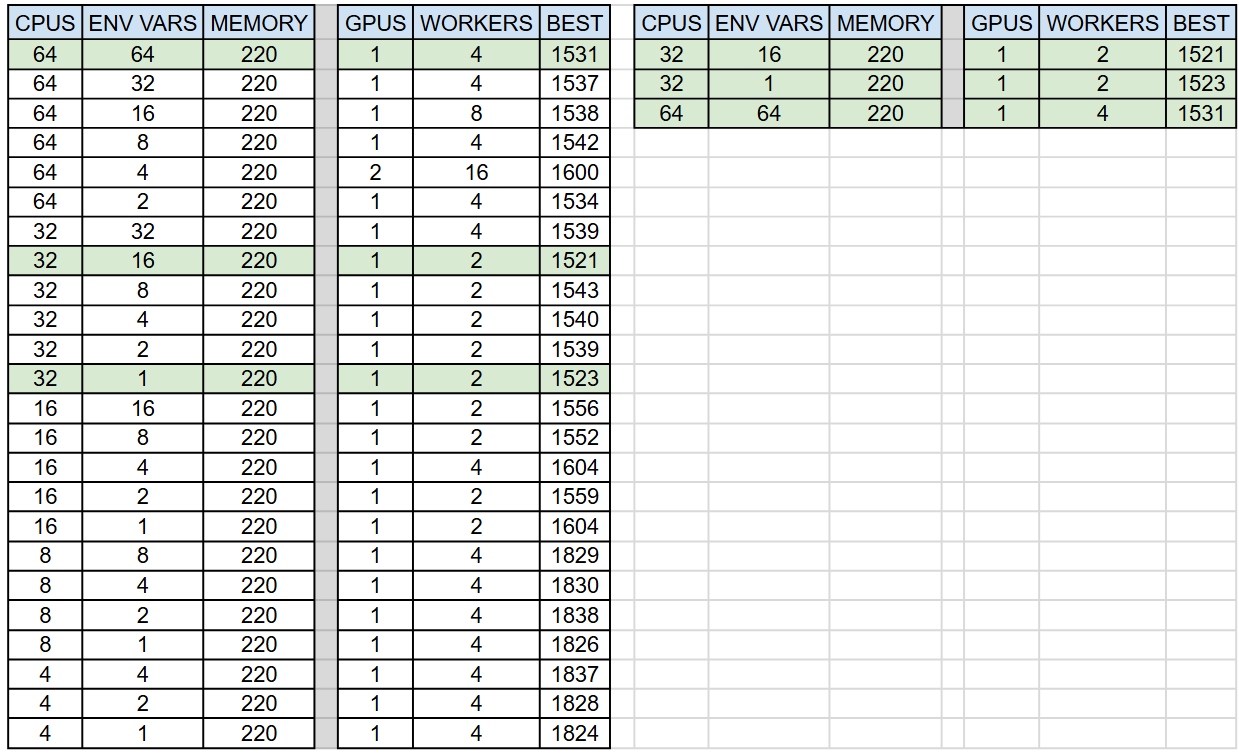
\includegraphics[width=\textwidth]{images/hpc-analysis.png}
    \caption{HPC tuning results for SLURM and environment-variable configurations (runtime reported in MMSS).}
    \label{fig:hpc-analysis}
\end{figure}

\subsubsection{Hardware}
We primarily used GPU-equipped HPC cluster nodes to execute the main experimental runs, as well as other resource-intensive environment and preprocessing tasks. The nodes provided the following hardware profile: 1--4 NVIDIA Tesla V100 GPUs (16~GB VRAM each), 64 CPU cores, and 256~GB DRAM. Reproduction on comparable hardware should yield similar end-to-end runtimes.

Running the full pipeline on systems without GPU support is generally impractical, except for a small, resource-friendly subset of experiments. Conversely, access to newer GPUs and/or larger VRAM capacity would substantially reduce runtime and expand the feasible experimental space. In our setting, several dimensions were intentionally constrained by available compute resources, including the number of datasets, the range of sample sizes, the set of computationally demanding algorithms, and the breadth of comparative analyses across sampling strategies.

\subsubsection{SLURM Configuration}
To optimize execution of the experimental pipeline, we conducted dedicated meta-experiments to characterize the behavior of our HPC environment under different SLURM configurations \cite{slurm}. This tuning was necessary because practical constraints such as job time limits and queueing overhead made efficient resource usage essential.

Although the nodes supported up to 4 GPUs, nearly 256~GB RAM, and all 64 CPU cores, allocating all available resources was not consistently optimal. For our workload, the best overall configuration used one GPU, 64~GB RAM, and all 64 CPU cores.

We further tuned thread- and process-related environment variables. The LensKit-specific variables were \texttt{LK\_NUM\_PROCS} and \texttt{LK\_NUM\_THREADS}; system-level variables were \texttt{OMP\_NUM\_THREADS}, \texttt{MKL\_NUM\_THREADS}, \texttt{OPENBLAS\_NUM\_THREADS}, and \texttt{NUMBA\_NUM\_THREADS}. For LensKit jobs, the best setting was \texttt{LK\_NUM\_PROCS}=32 and \texttt{LK\_NUM\_THREADS}=2 (i.e., half of available CPU cores in processes, with two threads per process), while the system-level thread variables performed best at 1. For RecBole jobs, the system-level thread variables performed best at 64.

Figure~\ref{fig:hpc-analysis} summarizes a subset of these tuning experiments. In each trial, we repeatedly executed a fixed experimental unit (one dataset, one sample size, and one algorithm) while varying only one factor at a time, either a single SLURM-related configuration parameter or a hardware-allocation variable. We also conducted limited checks of potential interactions between selected factors. The tested settings affected runtime but did not change ranking-metric outcomes.

\subsubsection{Project Setup}
The project was developed in a Linux-based environment as a standard Python software project and maintained under version control using local and remote Git repositories throughout the experimental lifecycle. In addition to a Python virtual environment, the workflow relied primarily on Singularity for reproducibility \cite{singularity}. The project includes both the container definition file and the generated image; however, the image itself is excluded from version control, together with other large or transient artifacts such as the virtual environment, external framework logs, runtime artifacts, and raw dataset files.

Early exploratory work briefly considered a Jupyter notebook-based structure, but this approach was discontinued in favor of a modular script-based codebase; the notebook artifacts therefore remain in the repository only for historical completeness and are not actively maintained. The repository is organized into dedicated directories: \texttt{artifacts} for temporary runtime files, \texttt{datasets} as the dataset placeholder, \texttt{docs} for LaTeX documentation projects, \texttt{output} for batch-job standard output and error logs, \texttt{results} for intermediate and aggregated result files and plots, \texttt{scripts} for sequential and parallel execution scripts, \texttt{singularity} for container definitions (and the untracked image), and \texttt{source} for the main Python modules. A \texttt{Makefile} serves as a self-documented command interface and substantially simplifies routine project operations, particularly SLURM job management.

\subsubsection{Dependencies}
Python 3.11 was required to ensure compatibility across the software stack; other interpreter versions produced dependency conflicts that could not be resolved reliably within our environment. To support reproducibility and standard dependency management practices, all package requirements were maintained in \texttt{requirements.txt} and mirrored in the Singularity definition.

Dependency management was centered on the two core recommender-system frameworks used in this work, LensKit and RecBole. At project setup time, these were pinned to LensKit 2025.2.0 and RecBole 1.2.1. Additional foundational libraries included \texttt{numpy}, \texttt{pandas}, \texttt{torch}, \texttt{scikit-learn}, and \texttt{matplotlib}. Rather than relying on automatic version resolution, we pinned these dependencies to fixed versions to prevent incompatibilities over time and preserve the stability of implemented methods.

\subsection{Configurations}
This subsection presents the configuration structure that implements the experimental design across all datasets, sample sizes, and algorithms while keeping comparisons methodologically consistent. The configuration structure is organized into clearly separated components: immutable constants for shared identifiers and naming conventions, experiment-level variables that specify evaluation and sampling behavior, model-level hyperparameters that control training behavior, and toolkit-specific execution settings for LensKit and RecBole. This separation enables controlled variation of the primary factor (interaction-data volume) while minimizing unintentional drift in other factors across runs. In addition, the subsection clarifies where parameters were fixed versus tuned, how common settings were mapped into each toolkit's API, and which compatibility-oriented adjustments were required to keep the full experiment matrix executable. Together, these design choices provide a traceable bridge from conceptual methodology to concrete implementation.

\subsubsection{Experiment Constants}
Core constants are defined in a dedicated module, primarily through Python \texttt{Enum} classes, to enforce type safety and naming consistency across the codebase. These include the \texttt{Tool} enum for toolkit selection, the \texttt{Dataset} enum for dataset identifiers aligned with repository structure, the \texttt{Sizing} and \texttt{Sampling} enums for sampling strategies, and the \texttt{Scorer} and \texttt{Model} enums for algorithm options in LensKit and RecBole. The same module also centralizes dataset feedback-type mappings, a whitelist of non-fatal runtime exceptions used for controlled failure handling, unified column names, display-name mappings, and shared file/directory naming conventions.

\subsubsection{Experiment Variables}
The \texttt{constants} module additionally defines experiment-level variables that control the study design. Key variables include a fixed recommendation cutoff of $K=10$ for $NDCG@K$, the train/validation/test split ratios, lists of fractional and absolute sample sizes, and an active mode represented as a pair consisting of one \texttt{Sizing} enum instance and one \texttt{Sampling} enum instance; together, this pair determines both the size-selection setting, whether fractional or absolute, and the sampling strategy.

\subsubsection{Hyperparameters}
Hyperparameters were intentionally constrained to computationally inexpensive settings to reduce per-run runtime and enable large experimental runs. For shared settings, both the LensKit crossfold partition count and epoch count were fixed at 1. For neighborhood-based models, the neighborhood size was set to $K=16$, with the minimum neighbor count aligned accordingly. For embedding-based models, the embedding dimension was fixed at 32. Additional model-specific parameters, including regularization strength, bias damping, confidence weighting, learning rate, and SVD interaction limits, were tuned during the environment-analysis meta-experiment presented in Figure~\ref{fig:hpc-analysis}.

\subsubsection{LensKit Configurations}
Within the LensKit pipeline, selected hyperparameters are mapped to algorithm-specific configuration dictionaries, while shared schema information, including unified column names and dataset feedback type, is imported from the \texttt{constants} module. Candidate generation uses \texttt{UnratedTrainingItemsCandidateSelector}, and history-lookup access is provided through \texttt{UserTrainingHistoryLookup}. Instead of the simplified \texttt{topn\_pipeline} helper, we use a pipeline builder to explicitly attach these components. Because LensKit does not expose a separate validation split in our setup, the predefined validation proportion is merged into the test proportion. Aside from this adjustment, implementation follows standard LensKit usage, with a minor adaptation to return $NDCG$ directly from the evaluation summary.

\subsubsection{RecBole Configurations}
In contrast to the LensKit workflow, the RecBole pipeline is centered on a single high-level training call parameterized by a centralized configuration object. Before execution, each sampled dataset is converted to RecBole's required \texttt{.atomic} format. Runtime configuration includes the tuned environment parameters and model hyperparameters, explicit use of the SGD learner, hardware-appropriate batch sizes, reduced \texttt{stopping\_step} and \texttt{eval\_step} values, and the predefined train/validation/test split ratios. To maintain compatibility across all selected settings and avoid algorithm-specific runtime failures, selected optional features, namely \texttt{enable\_amp} and \texttt{enable\_scaler}, were disabled.

\subsection{Structure}
This subsection summarizes the main source modules that implement the experimental pipeline. The codebase is organized by responsibility: experiment configuration and typed definitions, data loading and preprocessing, sampling, execution control across the parameter space, end-to-end run orchestration, result aggregation and persistence, and visualization and analysis. To support reproducibility and scalable execution in the HPC setting, the project also includes standardized job-control interfaces through \texttt{Makefile} targets and SLURM helpers, lightweight logging and diagnostics, and fault-tolerant utility routines for expected runtime issues. Together, these components connect raw interaction data to final comparative results while maintaining consistency across datasets, algorithms, and sampling conditions.

\subsubsection{Makefile}
The project \texttt{Makefile} \cite{make} provides standardized targets for environment management, including creation, activation, and deactivation of the Python virtual environment, dependency installation from \texttt{requirements.txt}, and execution of the primary experimental \texttt{run} module. It also includes targets for submitting and managing SLURM jobs, routine cleanup, result aggregation via the \texttt{aggregate} target executed by the \texttt{results} module, invocation of miscellaneous utilities, and plot generation to refresh figures from the most recent results file.

\subsubsection{parallel}
This module supports parallel execution within the SLURM environment by reading the adjacent \texttt{sequential.sh} batch script and programmatically appending a \texttt{tag} command-line argument before job submission. The \texttt{run} module consumes this tag to restrict execution to a specified subset of the experiment space, either an entire toolkit or a specific \texttt{toolkit:algorithm} pair, and the same tag is incorporated into the emitted results filename to keep outputs separated. The module then iterates over a predefined list of tags, submitting one batch job per tag. Two tagging schemes are supported: a single tag per toolkit, yielding two jobs, and a composite \texttt{toolkit:algorithm} tag, yielding $2\times 5 = 10$ jobs.

\subsubsection{constants}
This module centralizes a comprehensive set of constants that define most configuration settings; these are documented in detail in the dedicated \emph{Configurations} subsection above.

\subsubsection{load}
This module is primarily used for its \texttt{load} routine, which accepts a \texttt{Dataset} instance and an optional \texttt{parquet} flag indicating whether the dataset should be read from a \texttt{.parquet} representation; otherwise, a standard \texttt{.csv} file is loaded. Parquet is enabled by default due to its efficient on-disk storage and fast read performance. Prior to loading, a brief preprocessing step upcasts columns stored with the smallest compatible integer dtypes to ensure downstream operations behave correctly. In particular, unsigned integer fields are promoted to signed 32-bit integer types, and to signed 64-bit integer types when necessary, to avoid type-related errors in core functionality.

\subsubsection{logger}
This module provides a lightweight logging function that records timestamped messages and prepends a project-specific prefix for identification.

\subsubsection{plot}
This module serves as the primary plotting component for generating and updating all plots and figures. It reads the most recent results file and performs the typed computations and data extractions needed to produce the dataset description table, plots of raw performance values, plots of fully and partially normalized values, late-stage slope analyses, and elbow-point visualizations.

\subsubsection{results}
This module aggregates results generated by parallel job executions, merging multiple tagged results files into one combined results file. It also provides utilities to initialize an empty results instance and to save and load the most recent results from local storage.

\subsubsection{run}
This module serves as the main program entry point. It iterates over the predefined sample sizes, the included datasets, and the algorithms of both tools, and invokes the corresponding tool-specific execution method only for evaluations that are not yet present in the current aggregated results state. During execution, it records progress via logging, releases memory between runs as needed, and persistently saves intermediate outputs. In addition, the module provides configurable run options at the outset to enable selective execution over subsets of sample sizes, datasets, and tool--algorithm pair identifiers.

\subsubsection{sample}
This module contains the primary sampling method, together with supporting utility functions used exclusively by that method. These helper functions implement the stratified sampling variants, including the associated factor-cache mechanism described in detail in the \emph{Sampling} subsection.

\subsubsection{types}
This module centralizes dedicated type definitions, including nested types, to provide a compact specification. Most results- and plotting-related annotations are expressed using \texttt{TypeAlias} instances, accompanied by a small number of \texttt{TypedDict} definitions.

\subsubsection{use\_lenskit}
This module implements the \texttt{use\_lenskit} method, which provides the project's integration with LensKit. In addition, it defines a dictionary that maps \texttt{Scorer} enum instances to the corresponding configuration objects defined in the \texttt{constants} module, enabling instantiation of the appropriate LensKit scorer. The associated implementation and design decisions are discussed in the \emph{Configurations} subsection.

\subsubsection{use\_recbole}
This module implements the \texttt{use\_recbole} method, which provides the project’s integration with RecBole. It also includes an auxiliary helper function that serializes the specified dataset to an \texttt{.atomic} file when such a file is not already present. The \texttt{use\_recbole} method merges the relevant configuration parameters into a single dictionary, forwards them to RecBole, and returns the resulting NDCG score.

\subsubsection{utilities}
This module provides lightweight helper functions for diagnostics, robust execution, and preprocessing of user--item interaction data. For environment and file management, \texttt{gpu\_check} validates CUDA availability and enumerates detected GPUs, while \texttt{inter\_to\_csv}, \texttt{remove\_last\_column}, and \texttt{copy\_head} facilitate rapid inspection and restructuring of dataset files. To improve runtime stability, \texttt{safe\_run} executes callables under controlled exception handling by logging anticipated failures and re-raising unexpected exceptions, and \texttt{show\_memory} reports resident and virtual memory consumption during execution. Data integrity utilities include \texttt{check\_contiguous}/\texttt{make\_contiguous} to enforce 0-based contiguous identifier values and \texttt{check\_unique}/\texttt{make\_unique} to detect and resolve duplicate \texttt{(user\_id, item\_id)} pairs. The module further provides storage and reporting helpers, including \texttt{save\_parquet} in conjunction with \texttt{downcast\_dtypes} for compact dataset serialization, \texttt{check\_sparsity} for density and sparsity statistics, and \texttt{round\_significant} with \texttt{ceil\_significant} for consistent significant-figure rounding.

\subsection{Datasets}
This subsection outlines the dataset layer of the methodology, which forms the empirical basis of all subsequent experiments. Figure~\ref{fig:datasets} provides a compact summary of the main structural properties of the 11 datasets used in this study. The subsection further explains how the final set of large-scale public datasets was selected and acquired, how the source files were standardized and cleaned for compatibility with the pipeline, which storage and preprocessing optimizations were retained after practical evaluation, and how the resulting dataset abstractions were integrated into the main execution workflow. By making these dataset-related decisions explicit, the methodology clarifies both the scope of the empirical evidence and the data-processing steps required to ensure that comparisons across dataset sizes, algorithms, and toolkits remain systematically consistent.

\begin{figure}[H]
    \centering
    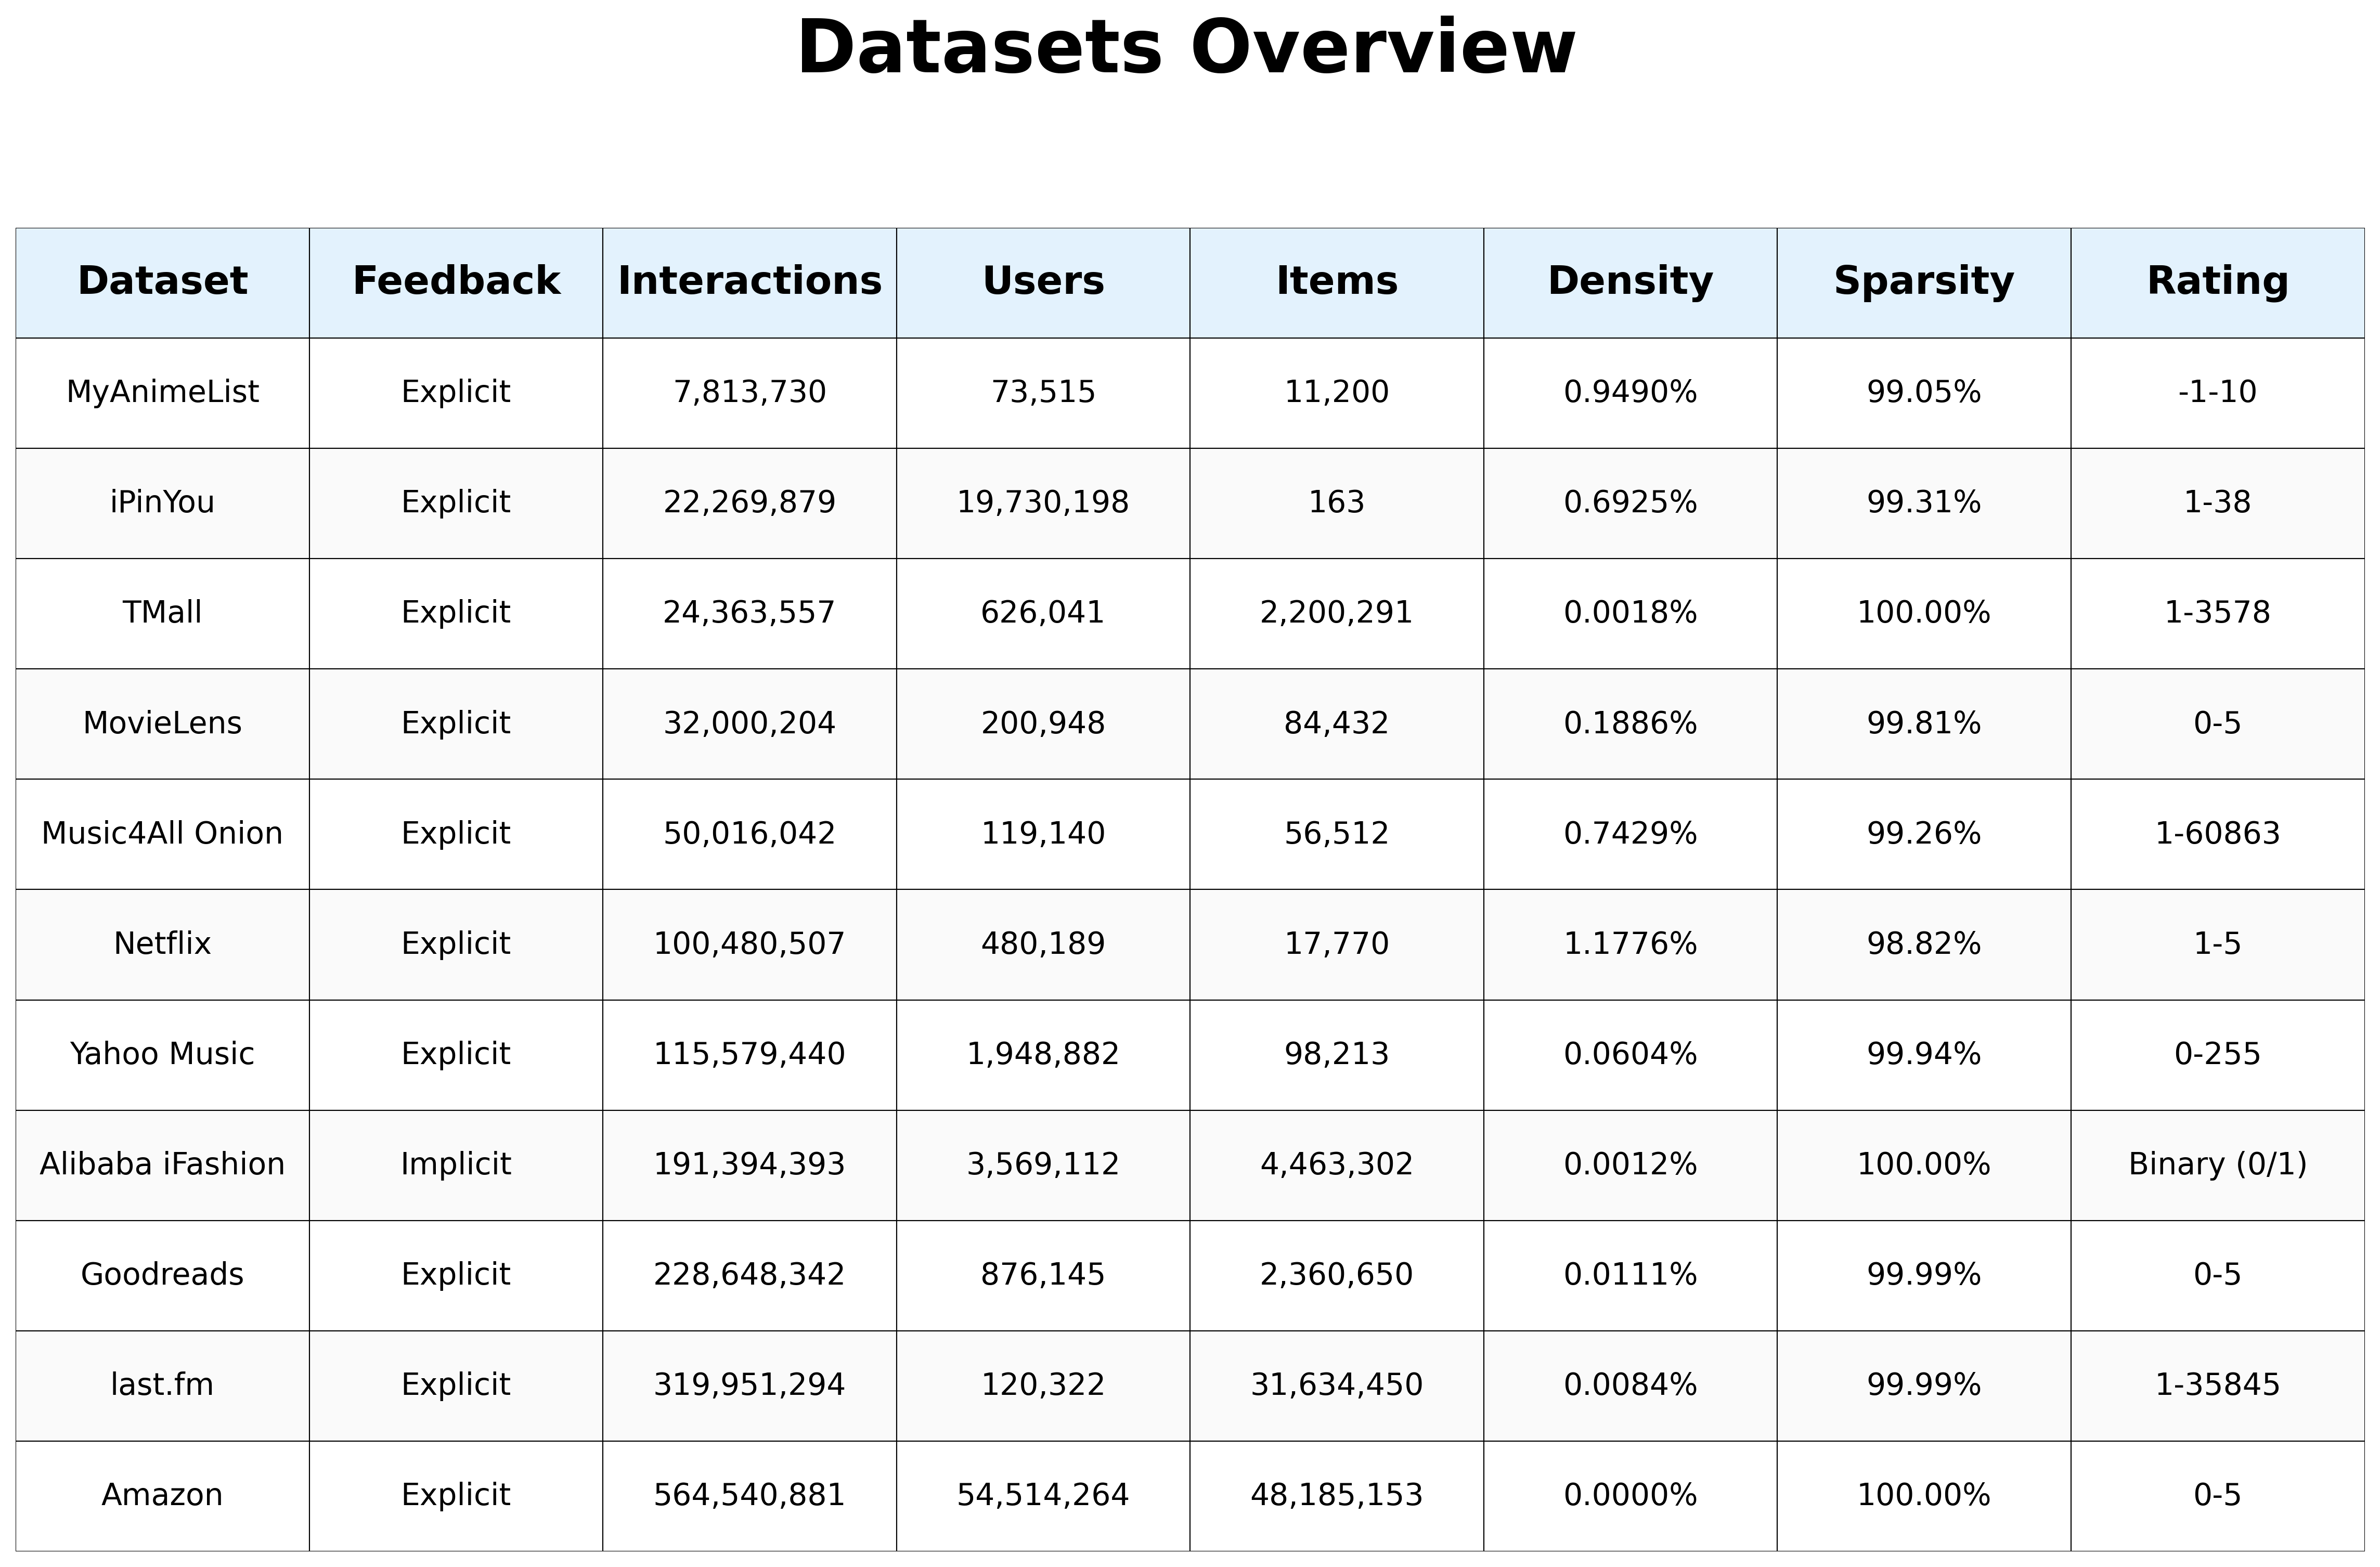
\includegraphics[width=\textwidth]{images/datasets.png}
    \caption{Metadata summary of the 11 datasets used in this study, reporting feedback type, interaction count, user count, item count, density, sparsity, and rating range}
    \label{fig:datasets}
\end{figure}

\subsubsection{Collection}
All datasets used in this thesis are publicly available and were obtained from a unified source maintained by the RecBole team \cite{recbole}. Metadata and dataset descriptions are provided through the official RecBole dataset repository \cite{recbole_datasets_repo} and the RecBole \emph{Datasets List} webpage \cite{recbole_datasets_page}, while the corresponding data files are distributed via the linked Google Drive resources.

At the time of collection, this source provided 43 datasets, with interaction counts ranging from approximately 10,000 to more than 1,000,000,000. To align dataset selection with the objective of this thesis---namely, analyzing recommender-system behavior under large-scale interaction data---datasets were prioritized by size and introduced incrementally during the project. The final selection includes 11 datasets, each containing at least 7 million interactions. This threshold is substantially above the initial minimum target of 1 million interactions and enables analysis across a broad range of large-scale dataset sizes.

The resulting corpus also preserves diversity across multiple dimensions. In terms of scale, datasets span from approximately 7 million to over 500 million interactions. In terms of feedback structure, the collection includes implicit-feedback data as well as several explicit-feedback formats, such as rating scales from $1$ to $5$ and from $0$ to $5$, as well as scales that include negative values, in addition to count-based behavioral signals such as clicks or listen counts. Domain coverage includes music, shopping, movies, books, and television-related platforms, and includes both widely used benchmark providers such as Amazon, Netflix, and MovieLens and less frequently studied sources.

Data acquisition was generally straightforward, with one major exception: the Amazon 2023 data. In available public distributions, this dataset is partitioned into 33 category-specific subsets (e.g., Books, Appliances), and no unified version was available for direct use. Therefore, a dedicated aggregation step was performed to merge all partitions into a single large-scale dataset. Because the raw combined data volume exceeds 500 million interactions, this process was storage-intensive and time-consuming. Although merging diverse product categories may introduce additional noise or cross-category effects, this decision was made intentionally, as the primary objective of this work is to investigate scale effects. Given the broader multi-dataset experimental design, this aggregated Amazon dataset serves as a useful high-volume case for exploratory analysis.

\subsubsection{Preparation}
After collection, each dataset was transformed into a standardized intermediate form before being used in the experimental pipeline. The source files were obtained from the RecBole team's linked Google Drive, specifically from the processed-datasets directory, where datasets are typically distributed as \texttt{.inter} files. In most cases, the source also provides a lightweight demo variant containing the header and the first few rows. These preview files were particularly useful because several of the full datasets were too large to inspect conveniently with standard text-editing tools. The demos therefore enabled rapid verification of the available columns, their order, and their data types prior to full preprocessing.

The preparation objective was to convert every dataset into a uniform CSV representation compatible with the project pipeline. To this end, all non-essential attributes, such as timestamps and other auxiliary fields, were removed. For explicit-feedback datasets, the retained columns were user identifier, item identifier, and rating; for the single implicit-feedback dataset, only the user and item identifiers were preserved. The resulting files were stored without a header row and with comma separation, using the standardized naming and column conventions defined in the \texttt{constants} module. Because these operations were repeated across datasets, the utilities module provides helper functions---\texttt{inter\_to\_csv}, \texttt{remove\_last\_column}, and \texttt{copy\_head}---to streamline the workflow while preserving the original raw \texttt{.inter} files. This approach maintained a clear separation between unmodified source data and the processed dataset versions used by the project, while also providing compact preview files for quick inspection of both raw and transformed data.

An additional preparation step concerned the enforcement of unique \texttt{(user\_id, item\_id)} pairs, which was required for compatibility with the full experimental pipeline. In particular, some LensKit algorithms did not operate correctly when duplicate interaction pairs were present. Duplicate detection and resolution were handled through the utility functions \texttt{check\_unique} and \texttt{make\_unique}. Only two of the eleven datasets---\texttt{MyAnimeList} and \texttt{iPinYou}---required this step, and each was treated according to the semantics of its feedback values. For \texttt{MyAnimeList}, where the interaction value is an explicit rating on a numerical scale from $-1$ to $10$, duplicates were resolved by retaining only the most recent occurrence for each repeated user--item pair. For \texttt{iPinYou}, by contrast, the interaction values represent count-like behavioral events, so duplicates were resolved by aggregating the corresponding values via summation for each repeated pair. This case-specific handling preserved the most meaningful interpretation of the data while ensuring a unique interaction table for downstream processing. Finally, each newly incorporated dataset required corresponding additions to the \texttt{constants} module, most importantly a new entry in the \texttt{Dataset} enum and a specification of whether the dataset provides explicit or implicit feedback.

\subsubsection{Optimization}
Because the selected datasets are large, preprocessing decisions had a substantial effect on both storage requirements and end-to-end runtime. We therefore evaluated several optimization strategies and retained only those that improved practical performance under our workload. One early approach was to enforce 0-based contiguous identifier ranges for user and item columns through the utility functions \texttt{is\_contiguous}, \texttt{check\_contiguous}, and \texttt{make\_contiguous}. The rationale was straightforward: since user and item identifiers primarily serve as keys, replacing sparse or alphanumeric identifiers with dense integer ranges from $0$ to $N-1$ can reduce storage requirements and permit the use of smaller integer \texttt{dtypes}. This transformation had little effect on datasets that were already contiguous, but for others---most notably Amazon, where identifiers are long alphanumeric strings---it substantially reduced file size, approximately halving the Amazon dataset from 20~GB to 10~GB.

Despite this storage benefit, contiguous remapping was not retained in the final workflow. In our practical runs, datasets subjected to this transformation tended to train more slowly rather than more quickly, contrary to the original expectation that smaller files would improve performance. Although this effect was not examined through a dedicated formal experiment, the observed increase in training time was sufficiently consistent and practically important that we decided against enforcing contiguous identifiers in the final pipeline.

The optimization strategy that proved most effective was the adoption of the \emph{Parquet} file format \cite{parquet}. This change required only minimal implementation effort through \texttt{pandas}' \texttt{to\_parquet} and \texttt{read\_parquet} functions, yet it yielded significant practical benefits: faster dataset loading during experiment execution and substantial reductions in storage size, comparable to those observed under contiguous remapping. The only disadvantage was reduced convenience for manual inspection in ordinary text editors; however, this had no meaningful effect on the execution of the experiments or on the validity of the results.

We also retained a second optimization related to data types. Motivated by the storage gains observed during the contiguous-remapping experiments, we isolated the \texttt{dtype} reduction component and implemented it independently through the \texttt{downcast\_dtypes} utility. This function scans all dataset columns and, for numeric columns only, applies \texttt{pandas.to\_numeric} with downcasting to more compact signed integer or floating-point representations where possible. The optimized datasets are then stored in Parquet format. To preserve compatibility with the subsequent experimental pipeline, integer columns smaller than 32-bit are upcast to \texttt{int32} during loading when required.

Taken together, these storage and loading optimizations also enabled a small but practically important refinement in runtime memory management. In an earlier version of the pipeline, the fully loaded dataset and the sampled subset were held simultaneously in separate \texttt{DataFrame} objects, which unnecessarily increased peak memory usage during experimentation. After the introduction of fast Parquet-based loading and lightweight \texttt{dtype} handling, this design was simplified so that, in each iteration, the dataset is loaded, sampled, and then replaced in memory by the sampled \texttt{DataFrame} passed to the subsequent module. This reduced avoidable memory pressure and left a larger share of the available memory budget to the training and evaluation procedures themselves.

\subsubsection{Integration}
Once collection, preparation, and optimization were in place, dataset handling became a uniform part of the main experimental loop. The \texttt{run} module iterates over the members of the \texttt{Dataset} enum and passes each dataset identifier to the loading, sampling, execution, and result-management components as required. This design keeps dataset-specific logic centralized in the configuration layer while allowing the remainder of the workflow to operate on a common interface.

The same dataset identifiers are also used consistently in auxiliary tasks, including persistence of intermediate outputs, retrieval of the latest aggregated results, and organization of dataset-specific runtime artifacts. As a result, the dataset layer functions not merely as an input source, but as a unifying abstraction that connects preprocessing decisions with the execution and storage logic of the overall experimental framework.

\subsection{Sampling}
This subsection defines how interaction-data subsets are constructed before model training and evaluation. The design combines two independent choices. First, sample size can be expressed either as a \emph{fractional} share or as an \emph{absolute} count. Second, rows can be selected using either random sampling or a stratified variant. Because this work studies performance as a function of data volume, the sampling pipeline is deterministic via a fixed seed, scalable to very large datasets, and sufficiently flexible for controlled re-runs under alternative sampling configurations.

\subsubsection{Sizing}
In this project, sizing is defined in conjunction with the sampling strategy and determines how the target sample size is computed from the full \texttt{pandas.DataFrame}. Two sizing modes are supported: fractional and absolute. In \emph{fractional} sizing, the sample size is expressed as a proportion of the full dataset and represented by a real-valued parameter in $(0,1]$. In \emph{absolute} sizing, the sample size is specified directly as a fixed number of entries in $[1, N]$, where $N$ denotes the total number of entries in the full dataset. Consistent with the overall configuration design, both modes are implemented as options in the \texttt{Sizing} enum.

\subsubsection{Random}
Within the experimental workflow, random sampling is applied in two places using \texttt{pandas.DataFrame.sample} with a fixed global random seed, which is one of the experiment variables defined in the \emph{Configurations} subsection. The first use occurs when random sampling is selected as the primary strategy. The second use appears as a post-processing step within stratified sampling, where random truncation is applied only when the combined groups exceed the target sample size.

\subsubsection{Stratified}
Stratified sampling is implemented using \texttt{groupby(...).sample(...)} over users or items, and optionally both, to form a hybrid strategy. For fractional sizing, the implementation is straightforward: the target fraction is applied per group. For absolute sizing, however, naively reusing the global fraction $\texttt{size}/N$ within each group produces a systematic shortfall in the final number of sampled rows. This occurs because each group contributes an integer number of rows after internal rounding, and many small groups contribute less than the expected fractional mass. In preliminary runs of the earlier implementation, this undershooting was substantial at scale; for example, target absolute sizes such as $1{,}000{,}000$ or $25{,}000{,}000$ often produced materially smaller samples, and in extreme cases, outputs far below the requested absolute size. A clear example is the \texttt{iPinYou} dataset: despite an absolute target grid beginning at $100{,}000$, archived run outputs for this dataset included sample sizes of only 1, 10, and 88, and in one case 0, demonstrating an extreme shortfall relative to the target size.

To address this issue, the final implementation introduces dataset- and target-specific factors represented by the \texttt{Factors} type alias. For each absolute target size, the effective groupwise fraction is scaled as \(\texttt{fraction} \times \texttt{factor}\). If no factor is known, sampling is repeated while increasing the factor multiplicatively by \(1.05\), rounded to two decimal places, until the realized sample size reaches or exceeds the requested absolute size. The discovered factor is then persisted in the factor cache and reused for the same dataset--size pair. A final random truncation step ensures that, when oversampling occurs, the obtained sample exactly matches the target size.

This factorized approach was chosen as a practical middle ground between two inadequate alternatives: the earlier no-factor method, which was computationally inexpensive but often substantially inaccurate in absolute-size mode, and explicit iterative allocation across groups, which was precise but more algorithmically complex and, at large scale, could introduce runtime overhead comparable to or greater than model-training time. In contrast, factorization preserves the simplicity of vectorized group sampling while reliably matching absolute target sizes after a one-time calibration phase.

\subsubsection{Options}
With sizing and sampling defined as separate \texttt{Enum} dimensions, the experimental design can be expressed as configurable combinations of \([\texttt{Fractional} \mid \texttt{Absolute}] \times [\texttt{Random} \mid \texttt{Stratified\_User} \mid \texttt{Stratified\_Item} \mid \texttt{Stratified\_Hybrid}]\). This decomposition keeps the implementation modular: size semantics and selection mechanics can be changed independently without modifying the surrounding workflow.

For the main experiment in this thesis, the selected default is \texttt{Absolute} + \texttt{Stratified\_User}. This choice provides a useful balance between preserving group representations and operational simplicity: it better preserves user demographics than fully random sampling, avoids the additional complexity of hybrid stratification in the default path, and works well with the factor-based correction mechanism for exact absolute targets. At the same time, the framework remains intentionally open: all other combinations are retained as first-class options, enabling straightforward reproduction, re-experimentation, and deeper sensitivity analyses under alternative sizing--sampling choices.

\subsection{Algorithms}
This subsection describes the recommender algorithms included in the experimental design and explains why they were selected. The project evaluates ten concrete tool--algorithm combinations in total: five through LensKit: \texttt{Popularity}, \texttt{ItemKNN}, \texttt{BiasedMF}, \texttt{ImplicitMF}, and \texttt{BiasedSVD}; and five through RecBole: \texttt{Pop}, \texttt{ItemKNN}, \texttt{BPR}, \texttt{NeuMF}, and \texttt{SimpleX}. This selection was intentionally kept small enough to remain computationally feasible at large data scale while still covering several distinct recommender-system families: non-personalized baselines, neighborhood methods, classical matrix factorization, pairwise ranking models, and neural collaborative-filtering approaches.

The chosen set also serves a comparative methodological purpose. Some algorithmic ideas are represented in both toolkits, most notably popularity and item-based $k$-nearest neighbours, which makes it possible to observe whether a broadly similar recommender idea demonstrates comparable scaling behavior across two different software implementations. At the same time, each toolkit also contributes methods that are more characteristic of its own ecosystem: LensKit contributes multiple matrix-factorization variants, whereas RecBole contributes ranking-oriented and neural models that are widely used in modern recommender systems research. Together, these ten combinations provide a sufficiently varied yet still manageable basis for studying how recommendation performance changes as interaction-data volume increases.

\subsubsection{Popularity}
Popularity was included in both LensKit and RecBole as the simplest baseline in the full experimental design. In principle, this algorithm does not attempt to learn personalized underlying patterns; instead, it recommends globally frequent or otherwise commonly interacted-with items. For this reason, it establishes a minimal reference point against which the value of more sophisticated models can be judged.

This baseline also served a practical diagnostic role in the pipeline. Because popularity-based recommendation is relatively straightforward, it was useful as an early sanity check for dataset preparation, runtime configuration, and end-to-end execution. If a particular dataset--size combination already produced long runtimes or unexpected failures under the popularity baseline, this was a strong indication that more complex models would be at least equally demanding or unstable. Including popularity in both toolkits therefore improved both the clarity and the robustness of the overall experimental design.

\subsubsection{Item KNN}
Item-based $k$-nearest neighbours was included in both LensKit and RecBole as the main neighborhood-based collaborative-filtering method. In contrast to the popularity baseline, ItemKNN produces personalized recommendations by identifying items that are similar to those a user has previously interacted with and then aggregating those item--item relations to score new candidates \cite{itemknn}. This approach is one of the most established recommender-system baselines and remains relevant because it is conceptually simple, interpretable, and often competitive in practice.

Within the context of this thesis, ItemKNN plays an important role because it represents a classical non-neural personalized recommender that is structurally different from matrix-factorization methods. Including the model in both toolkits improves comparability across implementations while also helping to determine whether data-scaling behavior is specific to embedding-based models or also appears in neighborhood-based algorithms.

\subsubsection{Biased Matrix Factorization}
Biased matrix factorization was represented in LensKit through two explicit-feedback variants: \texttt{BiasedMF}, trained with alternating least squares \cite{biasedmf}, and \texttt{BiasedSVD}, based on truncated singular-value decomposition of bias-adjusted residuals. Both belong to the broader family of matrix-factorization methods, where users and items are embedded in a lower-dimensional space and preferences are modeled through interactions between their learned embeddings.

The ALS-based BiasedMF implementation represents a classical large-scale matrix-factorization approach for explicit ratings and is included because it is a standard and well-established recommender baseline with known scalability properties. The BiasedSVD variant was included as a second explicit-feedback matrix factorization baseline within the same toolkit. Although simpler than iterative ALS optimization, it provides a useful contrast inside the embedding-based family and allows the evaluation to distinguish between two related but not identical implementations of biased matrix factorization.

\subsubsection{Implicit Matrix Factorization}
Implicit matrix factorization was included through LensKit's \texttt{ImplicitMF} implementation. Unlike the explicit-feedback factorization models above, this method is designed for settings in which observed interactions primarily indicate positive evidence with varying confidence rather than direct preference scores \cite{implicitmf}. This distinction is important for the present study because the dataset collection contains both explicit and implicit interaction formats, and a methodology centered only on explicit-rating models would therefore be too narrow.

Including ImplicitMF broadens the algorithm set beyond rating-prediction-oriented methods and permits a more suitable treatment of implicit datasets within the LensKit portion of the pipeline. It also provides a useful comparison against RecBole's implicit-feedback models, even though the underlying training objectives are not identical.

\subsubsection{Bayesian Personalized Ranking}
Bayesian Personalized Ranking (BPR) was included through RecBole as a classic pairwise-ranking method for implicit feedback. Rather than optimizing a pointwise prediction target, BPR learns from relative preferences by encouraging observed user--item interactions to rank above unobserved ones. This makes it particularly relevant for top-$k$ recommendation settings, where the ordering of candidate items matters more directly than the prediction of absolute rating values \cite{bpr}.

In the present methodology, BPR contributes a ranking-oriented factorization baseline that differs from both neighborhood-based recommenders and the more prediction-oriented LensKit matrix-factorization models. Its inclusion therefore improves coverage of the algorithm-design space without substantially increasing implementation complexity.

\subsubsection{Neural Collaborative Filtering}
Neural Collaborative Filtering was included through RecBole in the form of \texttt{NeuMF}. This model replaces the fixed inner-product interaction used in classical matrix factorization with a learnable neural interaction function, thus representing the deep-learning-oriented end of the selected algorithm spectrum \cite{neumf}. In methodological terms, it provides a useful contrast to the simpler embedding-based and neighborhood-based models by introducing a more expressive, non-linear user--item interaction mechanism.

Its inclusion was important because a study of scaling behavior that omitted modern neural recommenders would be incomplete. At the same time, only one neural model from this family was retained in order to keep the experimental design computationally feasible at very large sample sizes.

\subsubsection{SimpleX}
SimpleX was included through RecBole as a comparatively recent collaborative-filtering baseline that is stronger than its conceptual simplicity might initially suggest. It was selected to represent a modern recommendation approach that remains lightweight in design while still incorporating design choices associated with recent implicit-feedback training, particularly in its treatment of contrastive learning and negative sampling \cite{simplex}.

Methodologically, SimpleX complements BPR and NeuMF by expanding the RecBole subset beyond one classical ranking model and one neural model. This improves diversity within the RecBole portion of the experiment matrix and helps reduce the risk that conclusions about scaling in that toolkit are overly tied to a single modern modeling assumption.

\section{Results}
\subsection{Terminology}
This subsection defines the key terms used throughout the results analysis. Because the same experimental outcomes are represented in several complementary forms---raw line plots, normalized line plots, scatter plots, slope summaries, and table-based summaries---a compact shared vocabulary is necessary to keep the interpretation consistent across figures.

\subsubsection{Instance}
A result \emph{instance} is the output of a single evaluation run for a specific
$(\text{tool}, \text{algorithm}, \text{dataset}, \text{sample size})$ combination.
For example, \texttt{LensKit--Popularity--MovieLens-25M} $\mapsto \mathrm{NDCG} \approx 0.11$.
In Figures~\ref{fig:lines-common} and \ref{fig:lines-distinct}, each plotted point $(x,y)$ corresponds to one instance, where
$x$ is the sample size and $y$ is the $NDCG$ value.

\subsubsection{Group}
A result \emph{group} is the collection of instances that share the same
$(\text{tool}, \text{algorithm}, \text{dataset})$ combination, varying only in sample size.
Equivalently, a group is a set of points $\{(x_i, y_i)\}_{i=1}^n$ with fixed
tool, algorithm, and dataset, while $x_i$ varies.
In Figures~\ref{fig:lines-common} and \ref{fig:lines-distinct}, each colored line corresponds to one group.

\subsubsection{Normalization}
For a given group $g$ with instances $\{(x_i, y_i)\}_{i=1}^n$, we normalize sample size and
$NDCG$ \emph{within that group} as
\[
x_i'=\frac{x_i-x_{\min}}{x_{\max}-x_{\min}},
\qquad
y_i'=\frac{y_i-y_{\min}}{y_{\max}-y_{\min}} .
\]
Here \(x_{\min}\) and \(x_{\max}\) are the minimum and maximum \(x\)-values within the group \(g\),
and \(y_{\min}\) and \(y_{\max}\) are the minimum and maximum \(y\)-values within the group \(g\).

\subsubsection{Late-Stage Slope}
For each min--max normalized group $g$, we extract a single \emph{late-stage slope} as follows.
Let $(x_2', y_2')$ be the point with maximal normalized sample size, i.e. $x_2' = 1$.
Choose $(x_1', y_1')$ as the point with the largest $x_1'$ such that
\[
0.1 \le x_2' - x_1' \le 0.3.
\]
The late-stage slope is then
\[
m_g = \frac{y_2' - y_1'}{x_2' - x_1'}.
\]

\subsubsection{Elbow Point}
Let $y_{\max} = \max_i y_i$ denote the maximum observed $NDCG@10$ in group $g$, and let $x_{\max}$ denote the largest sample size evaluated in that group. Fix a threshold $\tau \in (0,1)$; in the summary tables, we use $\tau = 0.85$. For the purposes of the results summaries, we operationalize the \emph{elbow point} as the smallest sample size for which performance reaches at least a $\tau$ fraction of the maximum,
\[
x_{\mathrm{elbow}} = \min\{x_i : y_i \ge \tau y_{\max}\}.
\]
When reported as a percentage, we use
\[
100 \cdot \frac{x_{\mathrm{elbow}}}{x_{\max}}.
\]

\subsubsection{Gain}
To quantify the practical benefit of using all available data, we compute a relative gain between a near-full baseline and the full-size instance. Let $x_{\max}$ denote the largest sample size evaluated for a group, and let $x_{\mathrm{base}}$ denote the evaluated sample size satisfying
\[
0.7x_{\max} \le x_{\mathrm{base}} \le 0.9x_{\max}
\]
that is closest to the midpoint $(0.8x_{\max})$ of that interval. If such a baseline exists and its performance $y_{\mathrm{base}}$ is positive, the gain is defined as
\[
\mathrm{gain}(\%) = 100 \cdot \frac{y_{\max} - y_{\mathrm{base}}}{y_{\mathrm{base}}},
\]
where $y_{\max}$ is the $NDCG@10$ observed at $x_{\max}$. If no suitable baseline exists, the gain is left undefined.

\subsection{Legends}
The following legend figures are referenced repeatedly throughout the remainder of this section. One legend maps colors to datasets, while the other maps colors to tool--algorithm pairs. Keeping these mappings fixed across figures makes it possible to compare patterns across multiple visualizations without repeatedly redefining the color scheme.

\subsubsection{Datasets}
\begin{figure}[H]
    \centering
    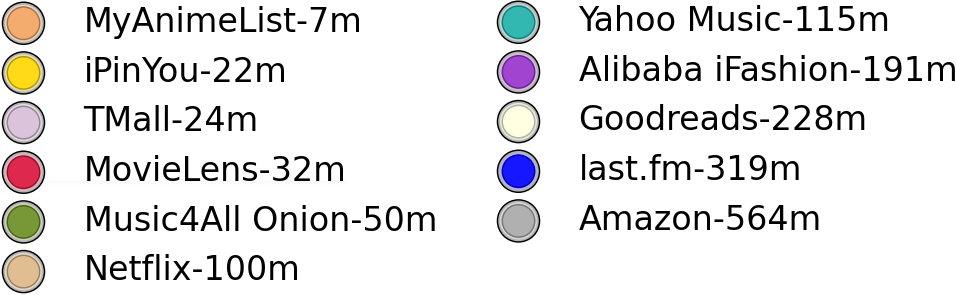
\includegraphics[width=0.60\textwidth]{images/legend-datasets.png}
    \caption{Dataset color legend.}
    \label{fig:legend-datasets}
\end{figure}

Figure~\ref{fig:legend-datasets} shows the color mapping used whenever lines or points are colored by dataset identity.

\subsubsection{Tool--Algorithm Pairs}
\begin{figure}[H]
    \centering
    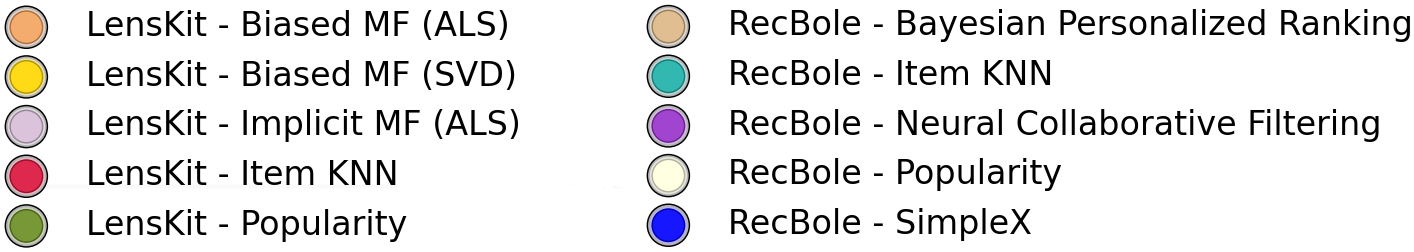
\includegraphics[width=0.85\textwidth]{images/legend-algorithms.png}
    \caption{Tool--algorithm color legend.}
    \label{fig:legend-algorithms}
\end{figure}

Figure~\ref{fig:legend-algorithms} shows the color mapping used whenever lines or points are colored by tool--algorithm pair rather than by dataset.

\subsection{Raw Results}
This subsection presents the observed $NDCG@10$ values against absolute sample size without any transformation of the underlying scales. The raw line plots therefore preserve the original magnitudes of both dataset size and recommendation performance. In these figures, color follows the dataset legend in Figure~\ref{fig:legend-datasets}, one line corresponds to one result group, and one point corresponds to one result instance. Some groups are only partially visible or absent because specific jobs did not complete within the imposed 24-hour runtime limit; this affected Amazon most strongly, followed by Alibaba-iFashion and, to a lesser extent, Last.fm. Even under that practical limitation, the dominant visual pattern across the raw figures is positive scaling: in nine of the ten algorithm panels, most groups tend to attain their best or near-best performance at the largest available sample sizes, with RecBole BPR being the main exception.

\subsubsection{Full Scale}
\begin{figure}[H]
    \centering
    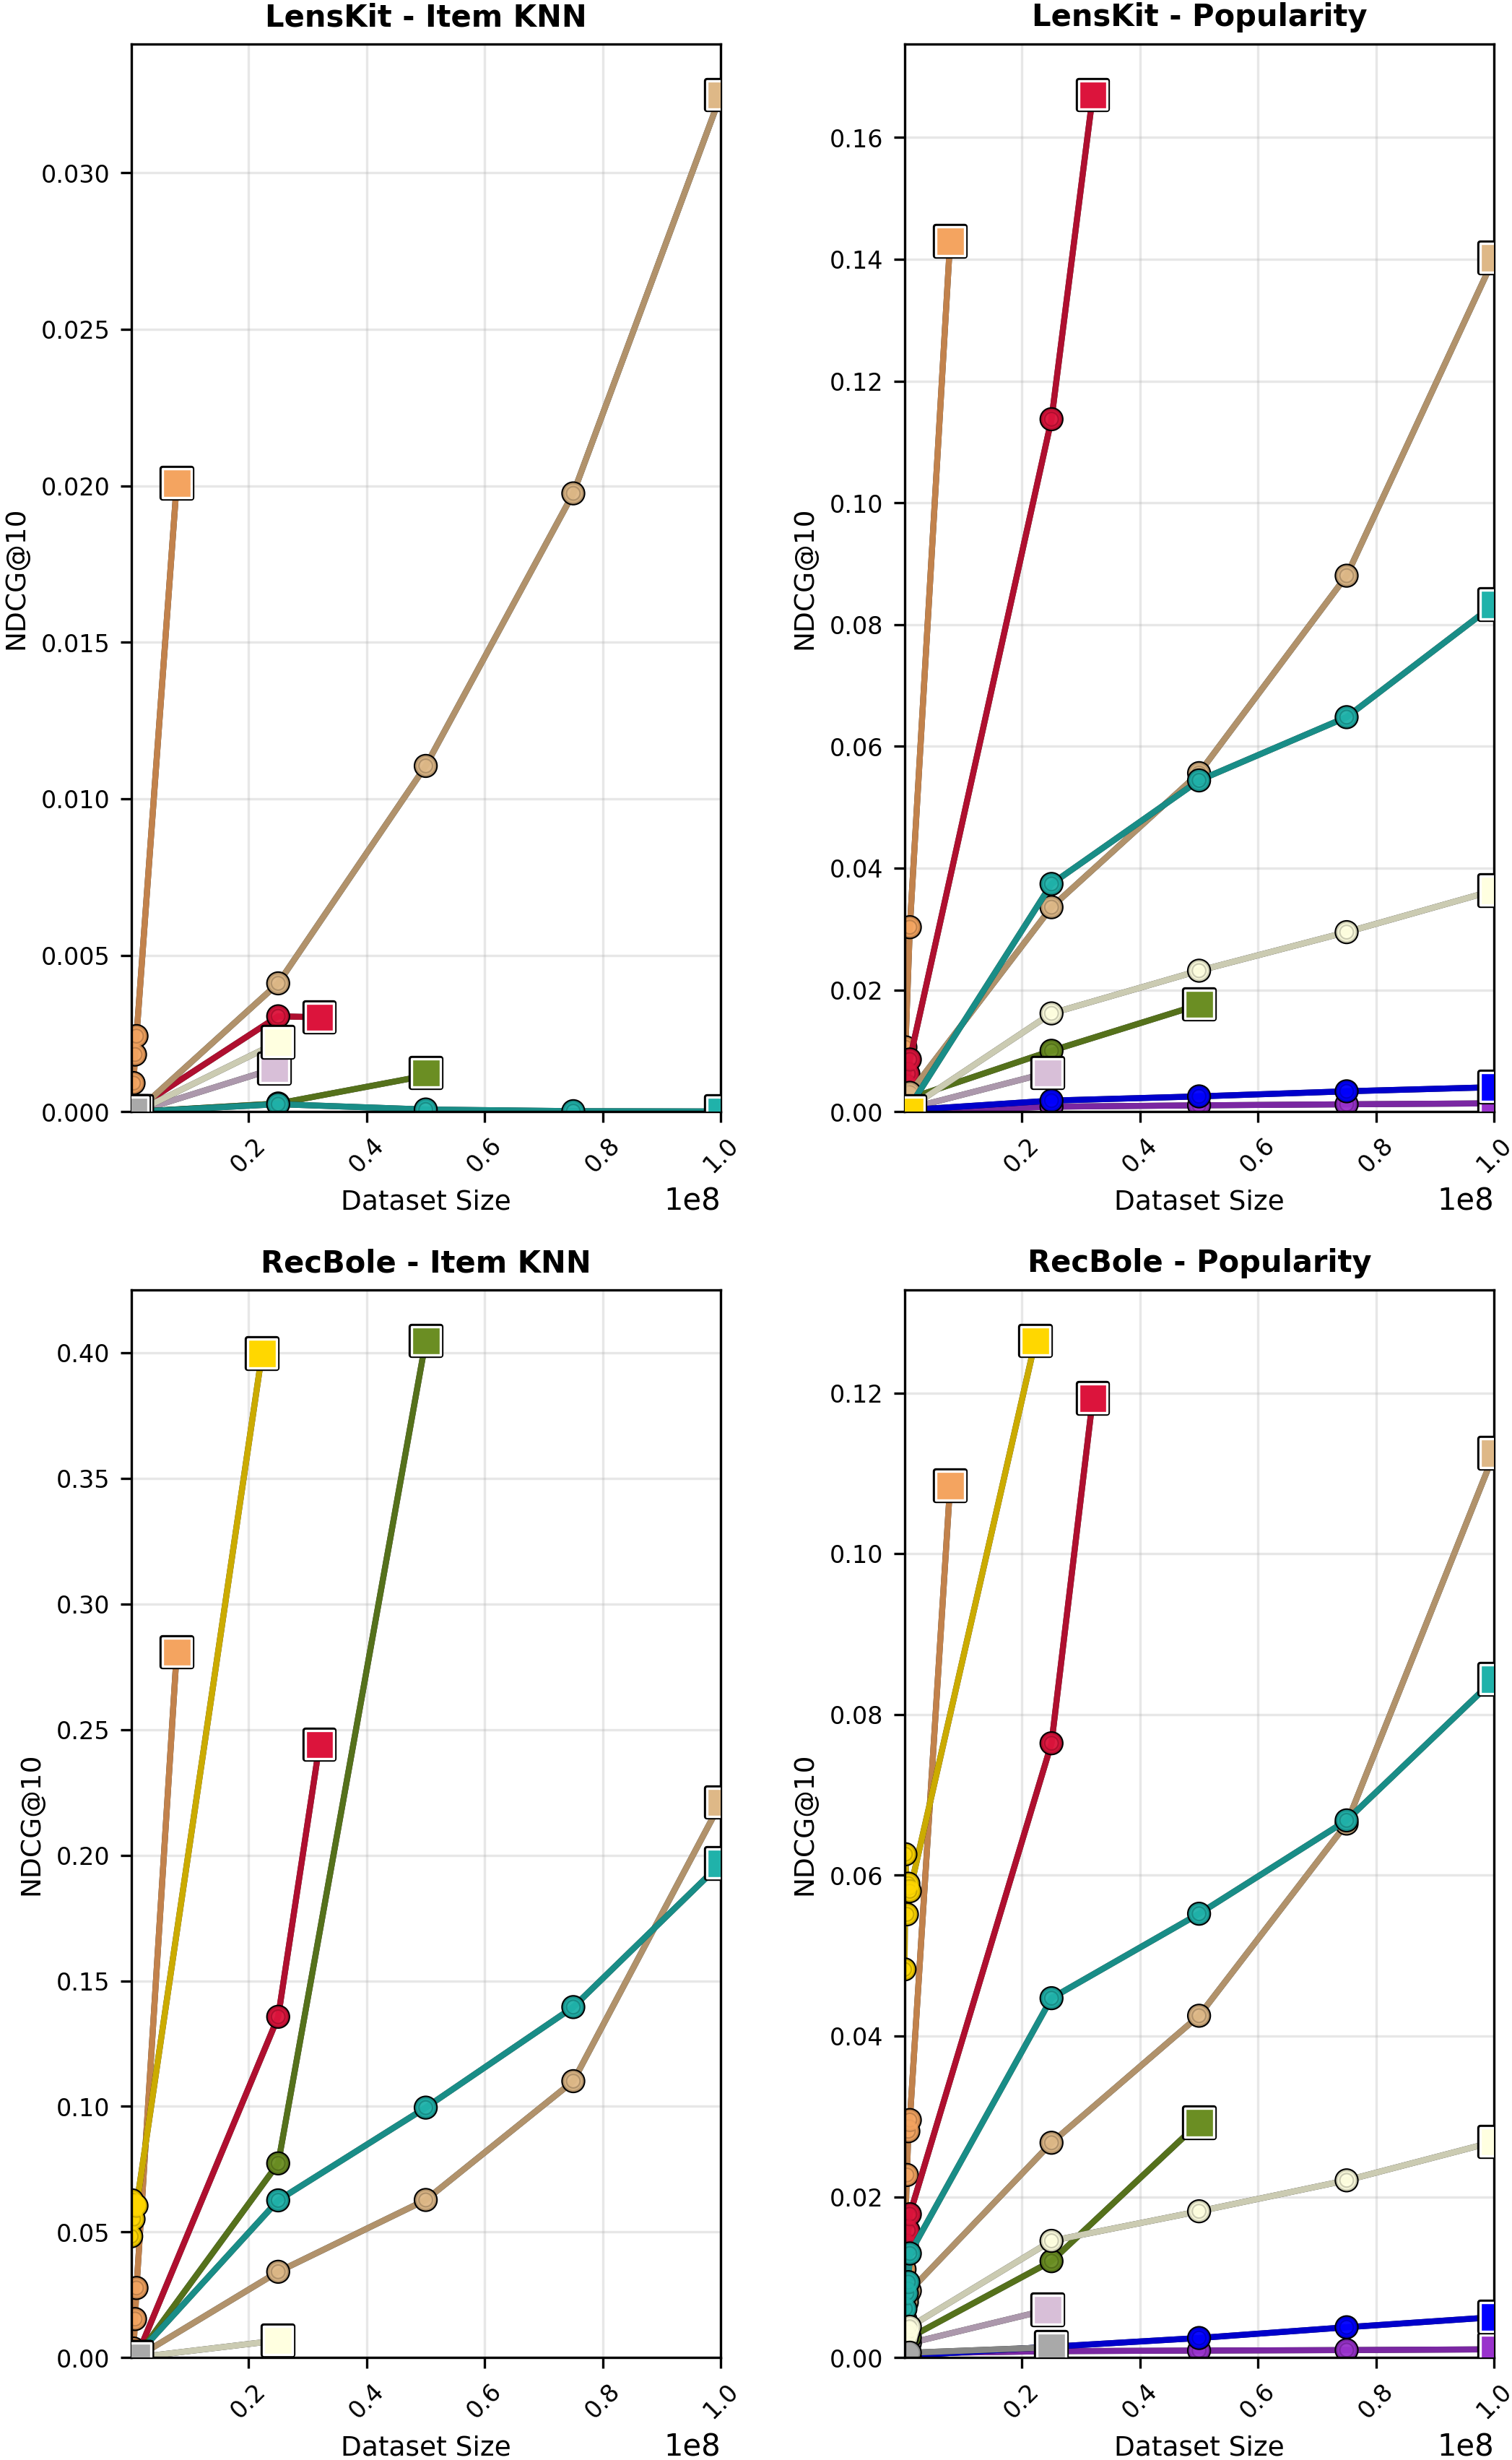
\includegraphics[width=0.7\textwidth]{images/lines-common.png}
    \caption{Raw $NDCG@10$ against absolute sample size for the two algorithms represented in both toolkits: Popularity/Pop and ItemKNN.}
    \label{fig:lines-common}
\end{figure}
\begin{figure}[H]
    \centering
    
\includegraphics[width=\textwidth]{images/lines-distinct.png}
    \caption{Raw $NDCG@10$ against absolute sample size for the remaining toolkit-specific algorithms: LensKit BiasedMF, ImplicitMF, and BiasedSVD, together with RecBole BPR, NeuMF, and SimpleX.}
    \label{fig:lines-distinct}
\end{figure}

Figures~\ref{fig:lines-common} and \ref{fig:lines-distinct} provide the most direct view of the measured values because they retain the original $NDCG$ scale. Across these panels, the dominant pattern is that the largest observed $NDCG$ values usually occur at the largest completed sample size, often the full dataset. One notable exception appears in LensKit ItemKNN on MovieLens, where performance does not continue to increase between the 25M sample and the full 32M dataset. Aside from such isolated cases, the raw plots suggest broadly monotonic or near-monotonic improvement for many groups, especially on MyAnimeList, iPinYou, MovieLens, Netflix, and Yahoo Music. The highest absolute values in the entire results set appear in the RecBole ItemKNN panel, where the iPinYou and Music4All Onion groups approach $NDCG \approx 0.40$ at their largest sizes. At the same time, the raw plots also show that absolute performance levels are highly dataset-dependent: a dataset with a smaller maximum sample size can still achieve a higher $NDCG$ than a much larger dataset, and vice versa. For that reason, the raw figures are most useful for inspecting within-group growth, not for inferring a general cross-dataset pattern from absolute peak heights alone.

\subsubsection{Zoomed View}
\begin{figure}[H]
    \centering
    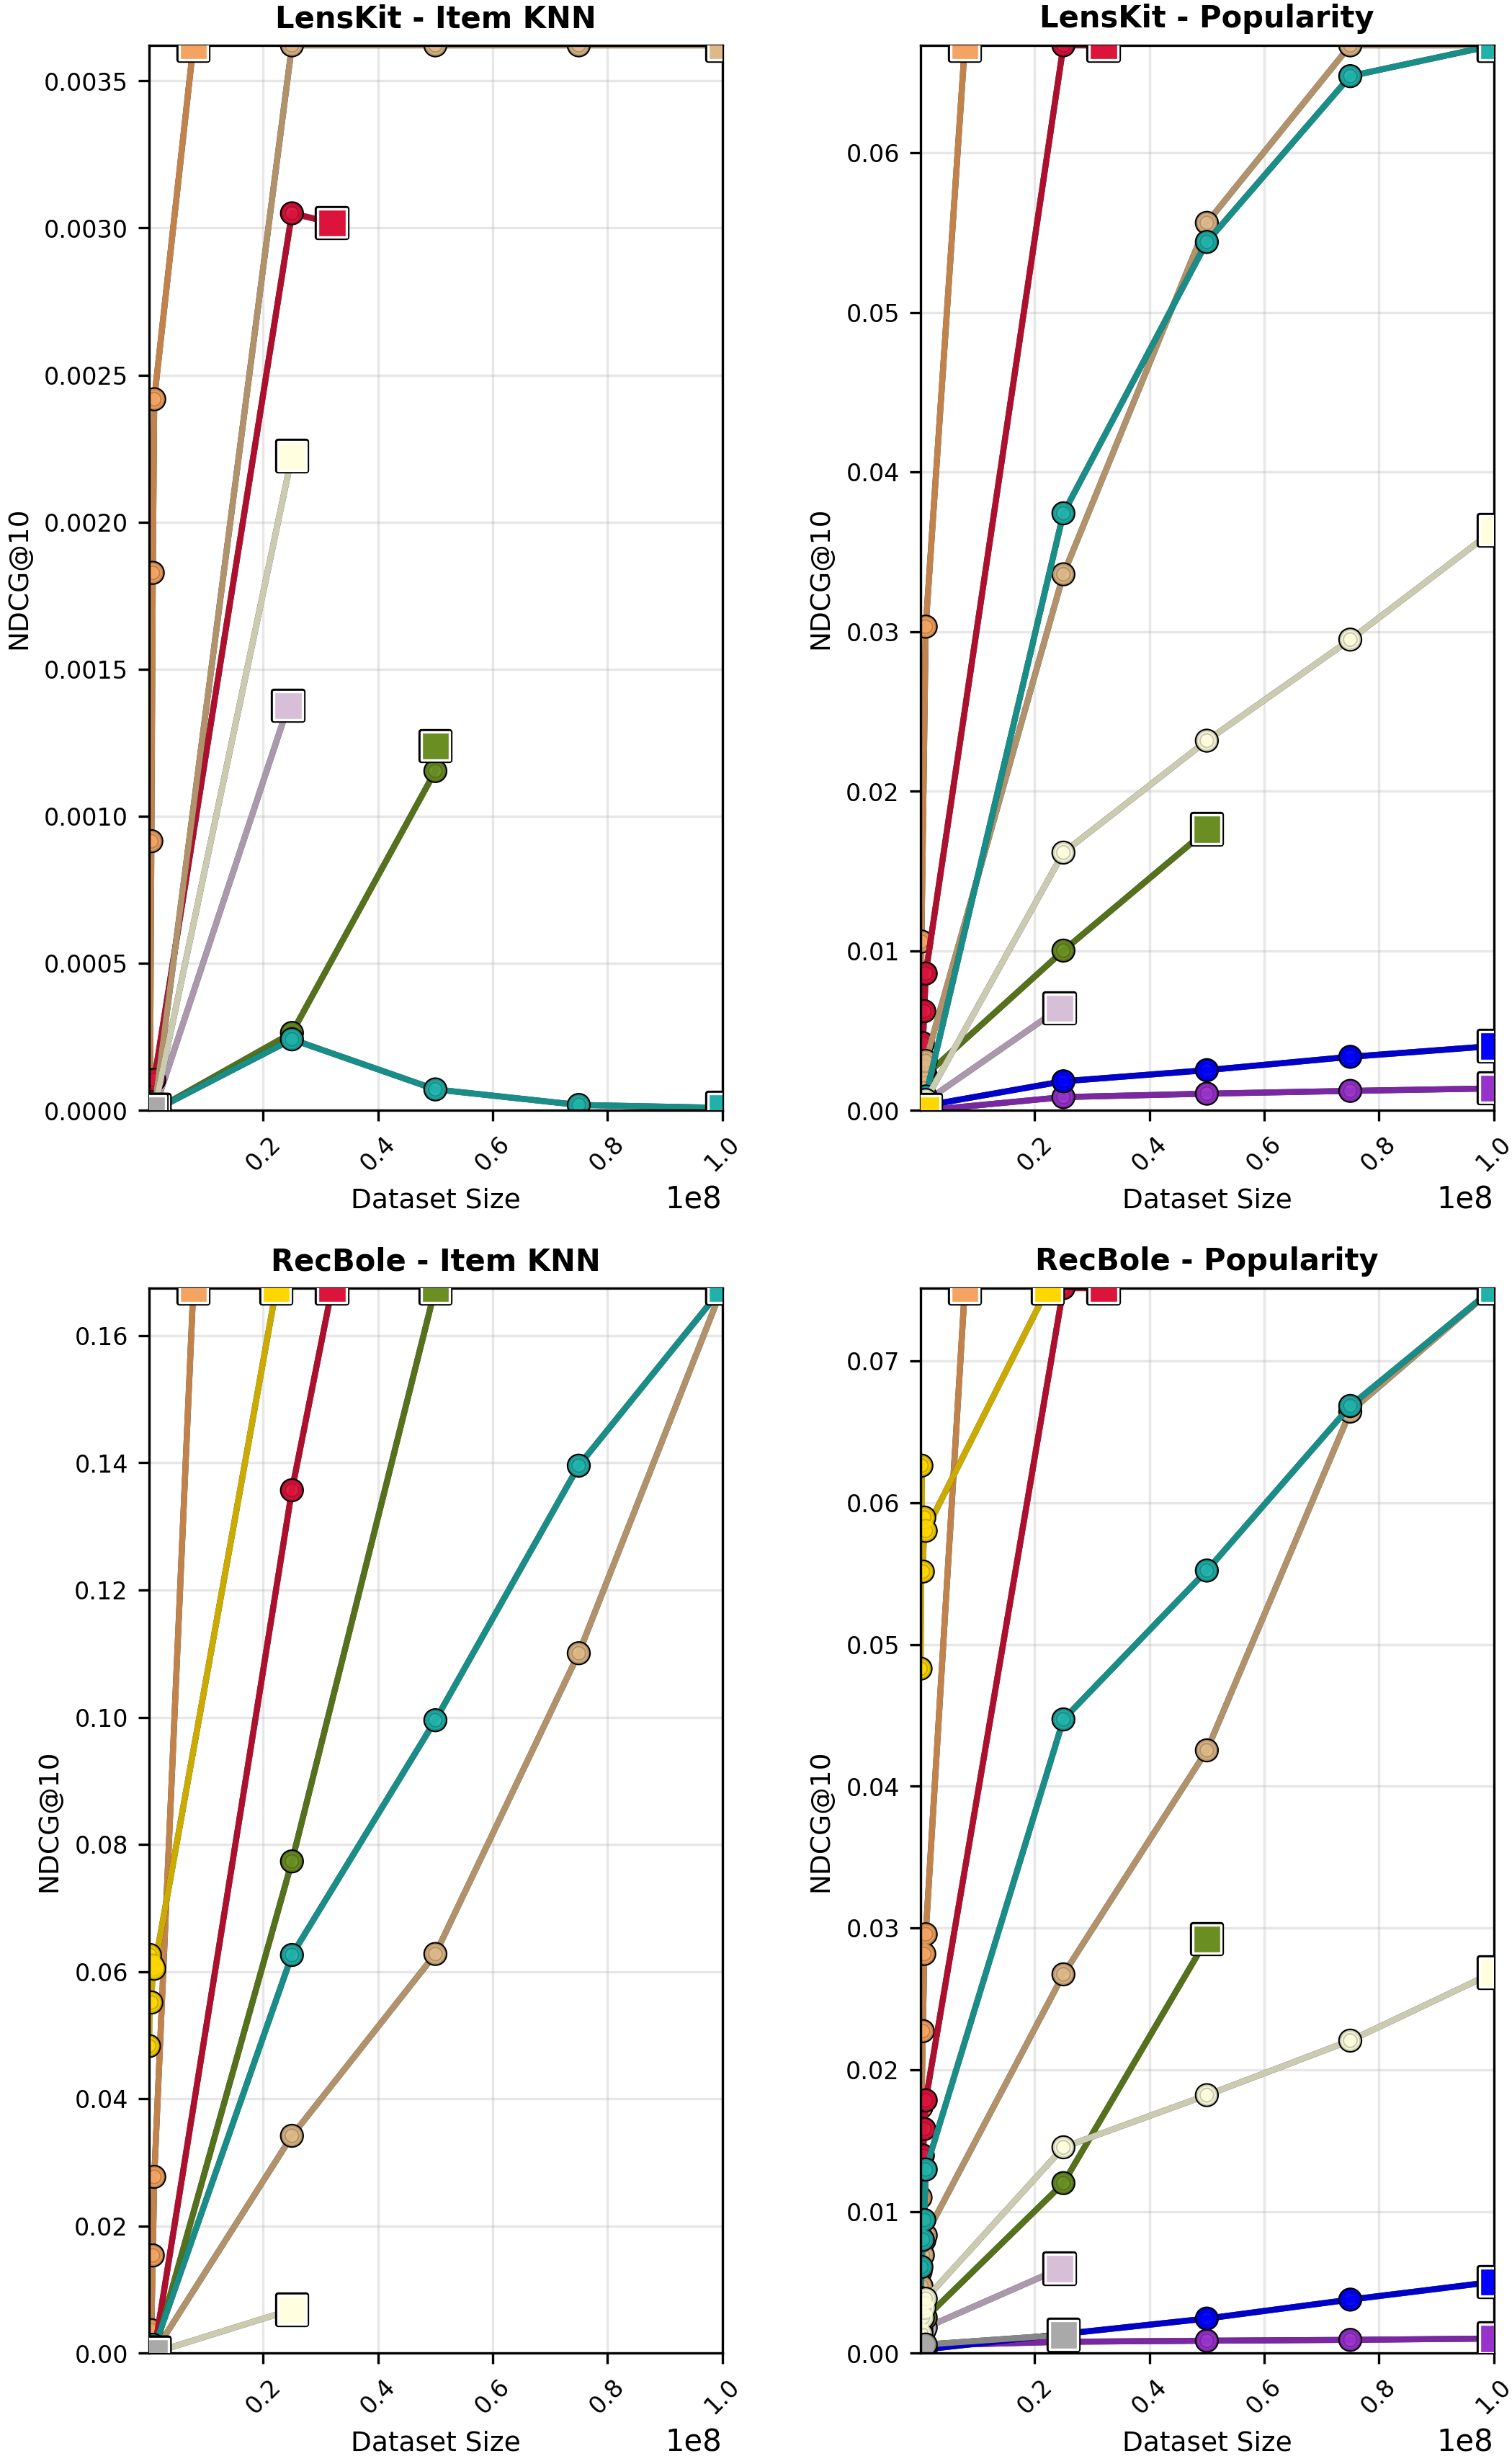
\includegraphics[width=0.7\textwidth]{images/lines-zoomed-common.png}
    \caption{Zoomed version of Figure~\ref{fig:lines-common}, emphasizing lower-valued raw $NDCG@10$ trajectories.}
    \label{fig:lines-zoomed-common}
\end{figure}
\begin{figure}[H]
    \centering
    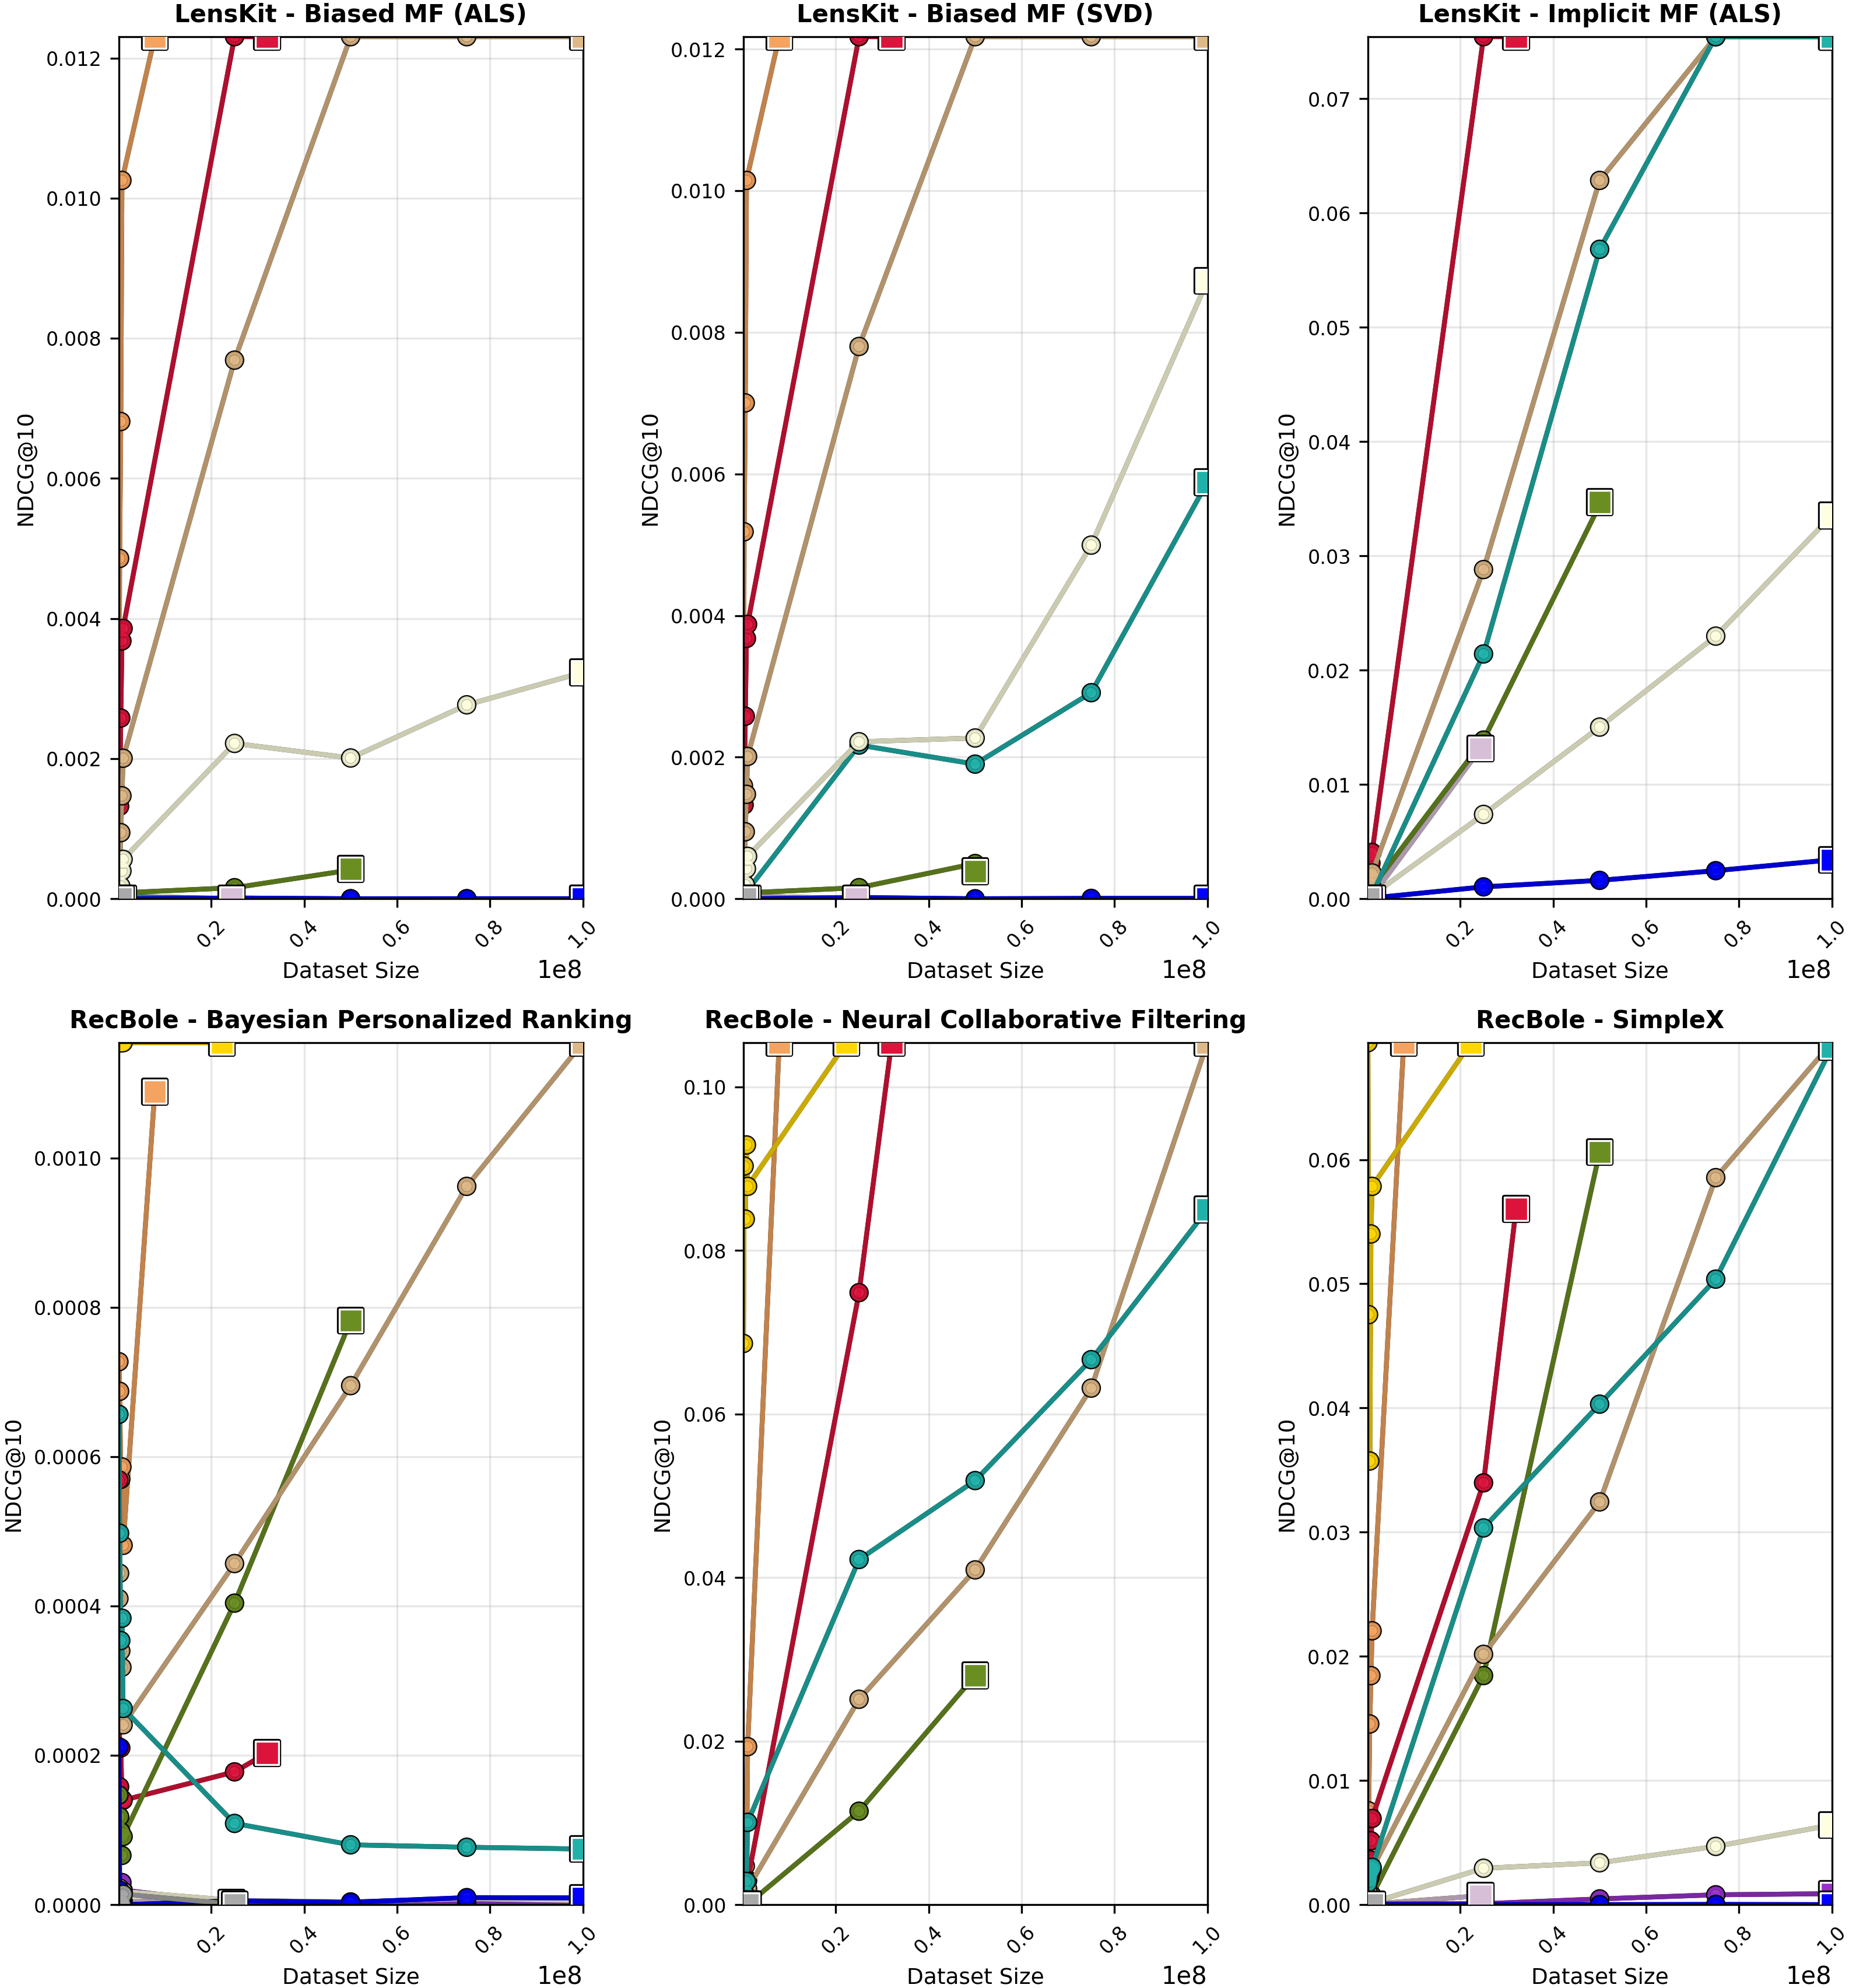
\includegraphics[width=\textwidth]{images/lines-zoomed-distinct.png}
    \caption{Zoomed version of Figure~\ref{fig:lines-distinct}, emphasizing lower-valued raw $NDCG@10$ trajectories.}
    \label{fig:lines-zoomed-distinct}
\end{figure}

Figures~\ref{fig:lines-zoomed-common} and \ref{fig:lines-zoomed-distinct} provide the same raw results after deliberately truncating the upper part of the $y$-axis. This sacrifices visibility of the highest-performing groups in order to make the lower-valued trajectories interpretable. The zoomed view is particularly useful for LensKit ItemKNN and RecBole BPR, where several groups would otherwise appear almost flat because a small number of much larger $NDCG$ values dominate the scale. Under this magnified view, additional positive scaling patterns become easier to identify, including several Music4All Onion and Goodreads groups. By contrast, Last.fm and Alibaba-iFashion still appear comparatively weak even after zooming, indicating that their lower performance is not merely a visualization artifact. The zoomed BPR panel also makes this otherwise sparse-looking set of trajectories easier to interpret: although most groups remain confined to a very low $NDCG$ range, BPR is not uniformly negative trends-wise, and datasets such as Netflix, Music4All Onion, and MyAnimeList still show upward movement with increasing size. Yahoo Music, however, stands out even within this already atypical panel as a conspicuous counterexample, exhibiting a clear decrease as size increases. Overall, the zoomed figures refine the interpretation of the raw plots, but they do not overturn the central observation that positive scaling dominates the results outside a limited set of outliers.

\subsection{Normalized}
The normalized visualizations transform both sample size and $NDCG$ to the $[0,1]$ interval within each group. This removes differences in absolute scale and makes the shape of each group's trajectory directly comparable to the others. The resulting figures are therefore more suitable than the raw plots for evaluating whether performance tends to rise, flatten, or decline as a function of relative dataset growth, even when the underlying datasets differ substantially in size or in attainable absolute $NDCG$.

\subsubsection{Line Plots}
\begin{figure}[H]
    \centering
    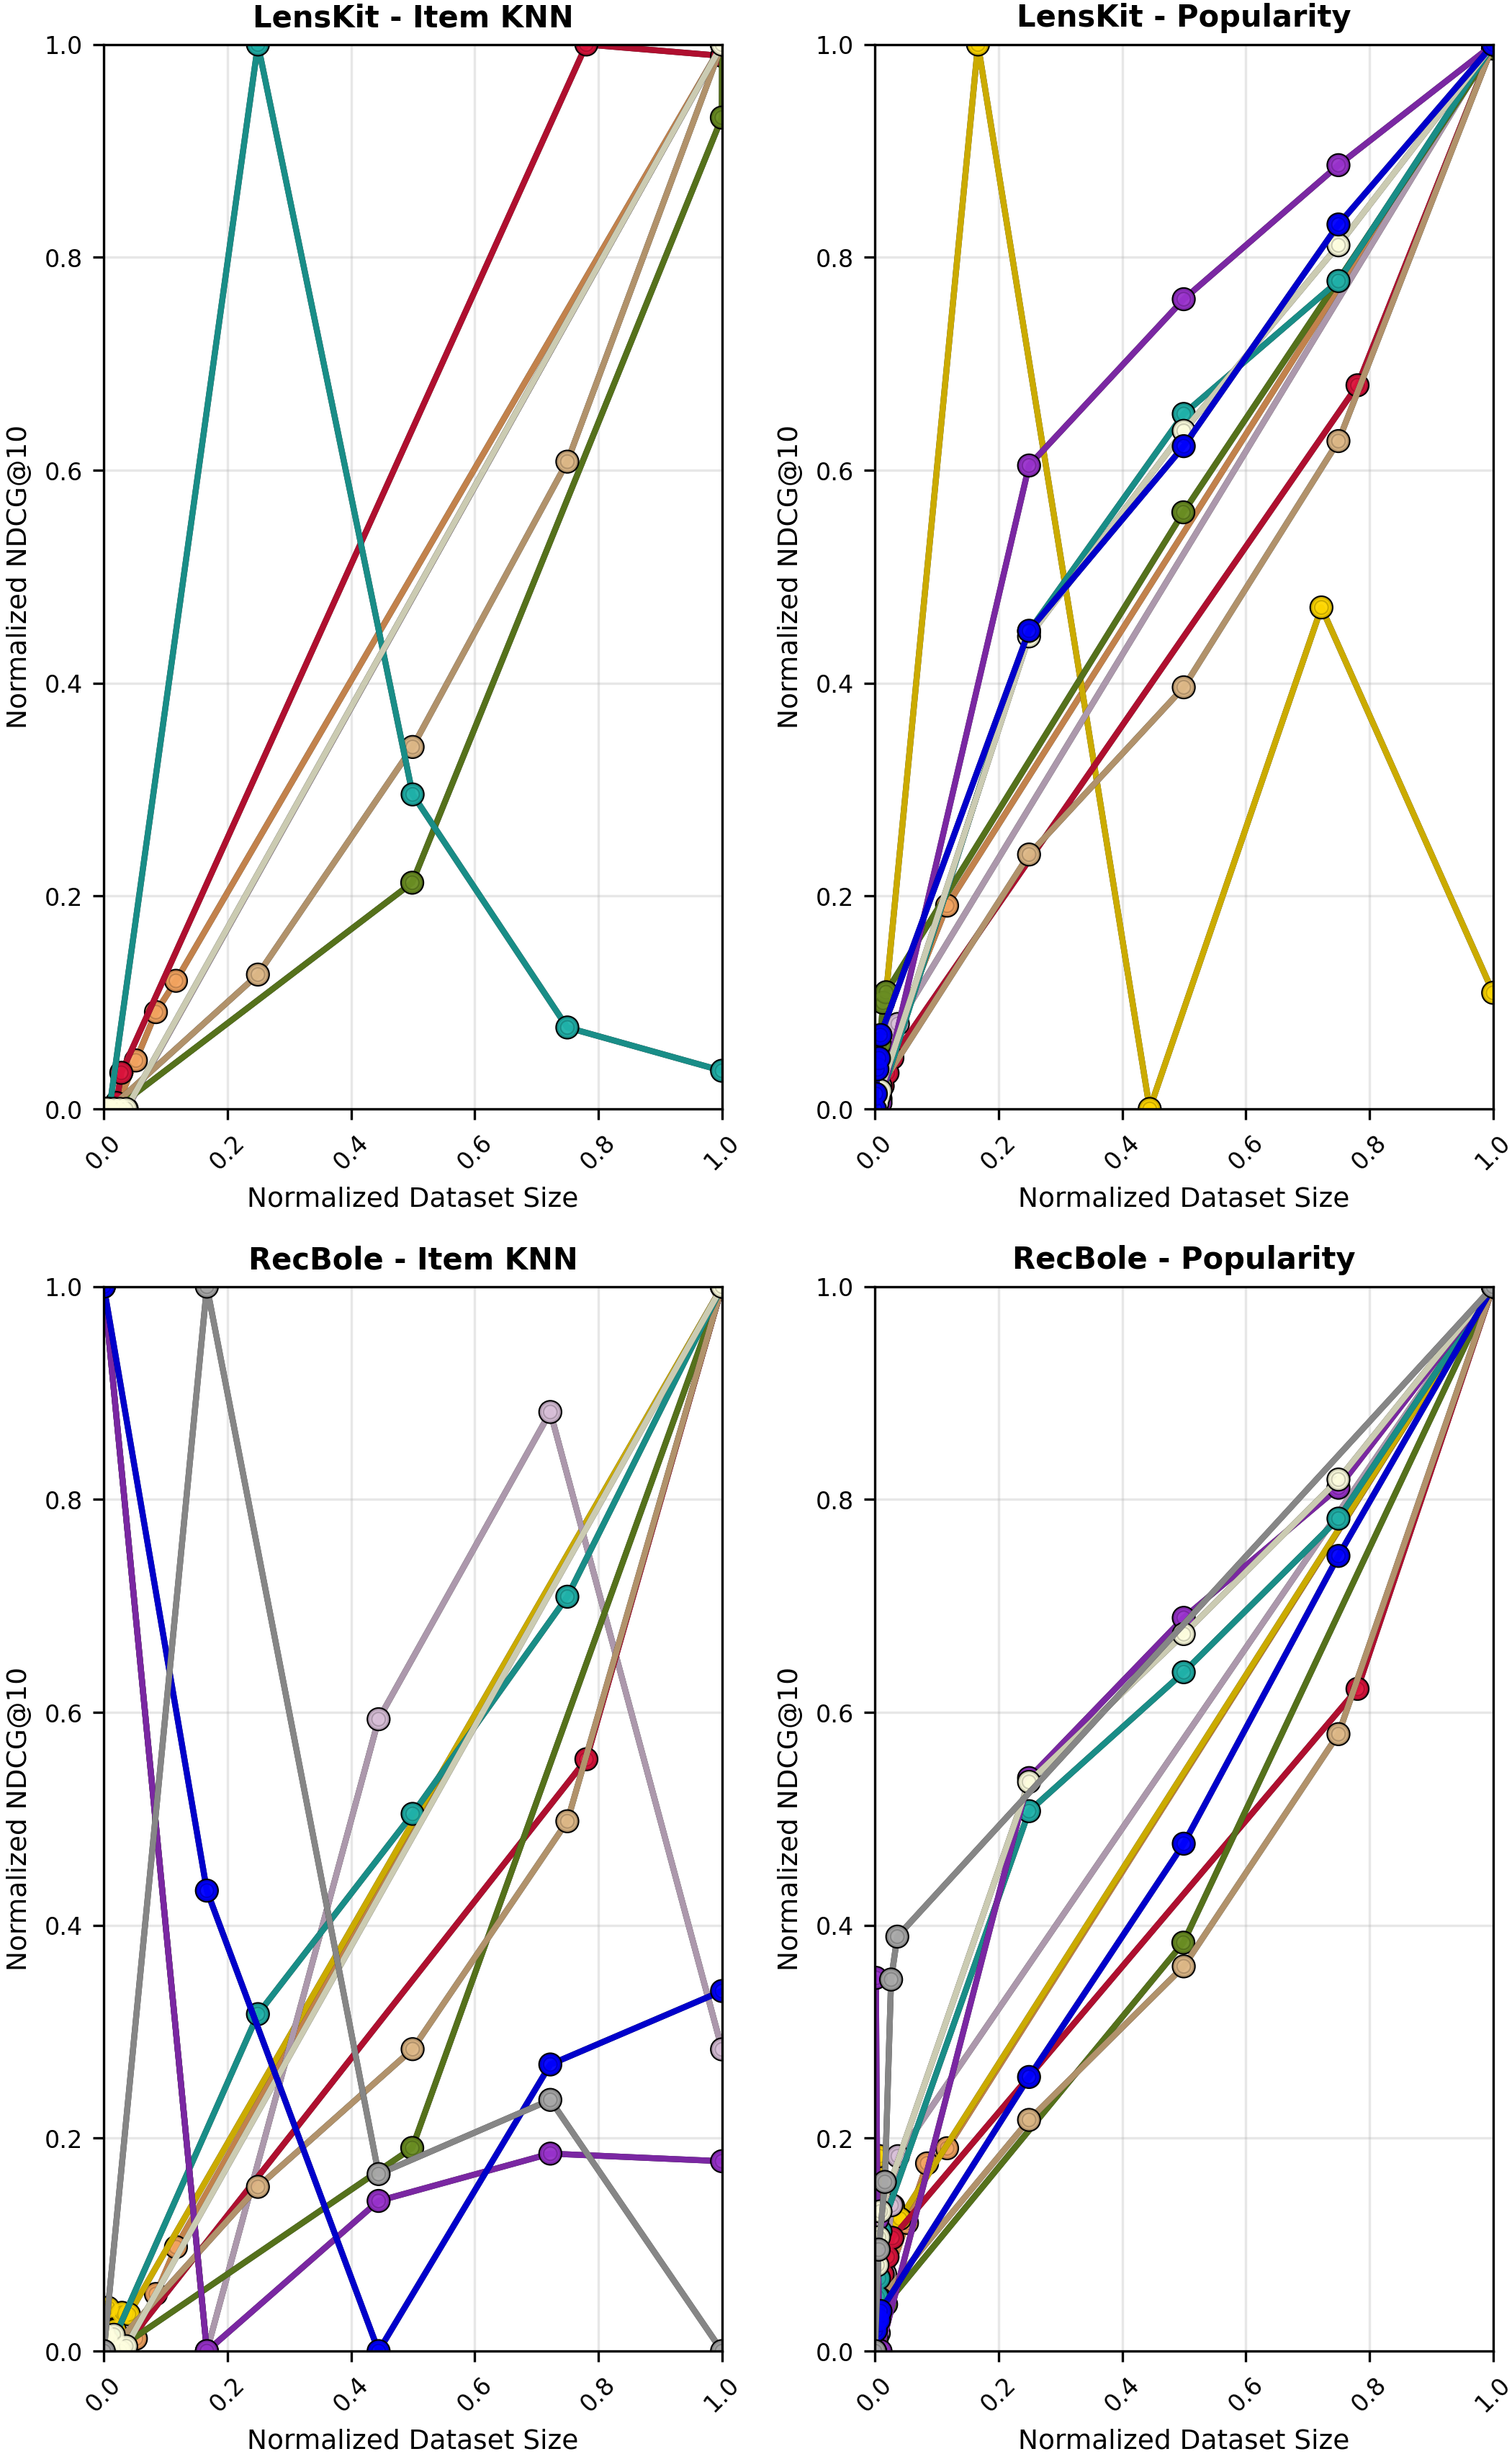
\includegraphics[width=0.7\textwidth]{images/normalized-common.png}
    \caption{Min--max normalized version of Figure~\ref{fig:lines-common}. Both sample size and $NDCG@10$ are normalized within each group.}
    \label{fig:normalized-common}
\end{figure}
\begin{figure}[H]
    \centering
    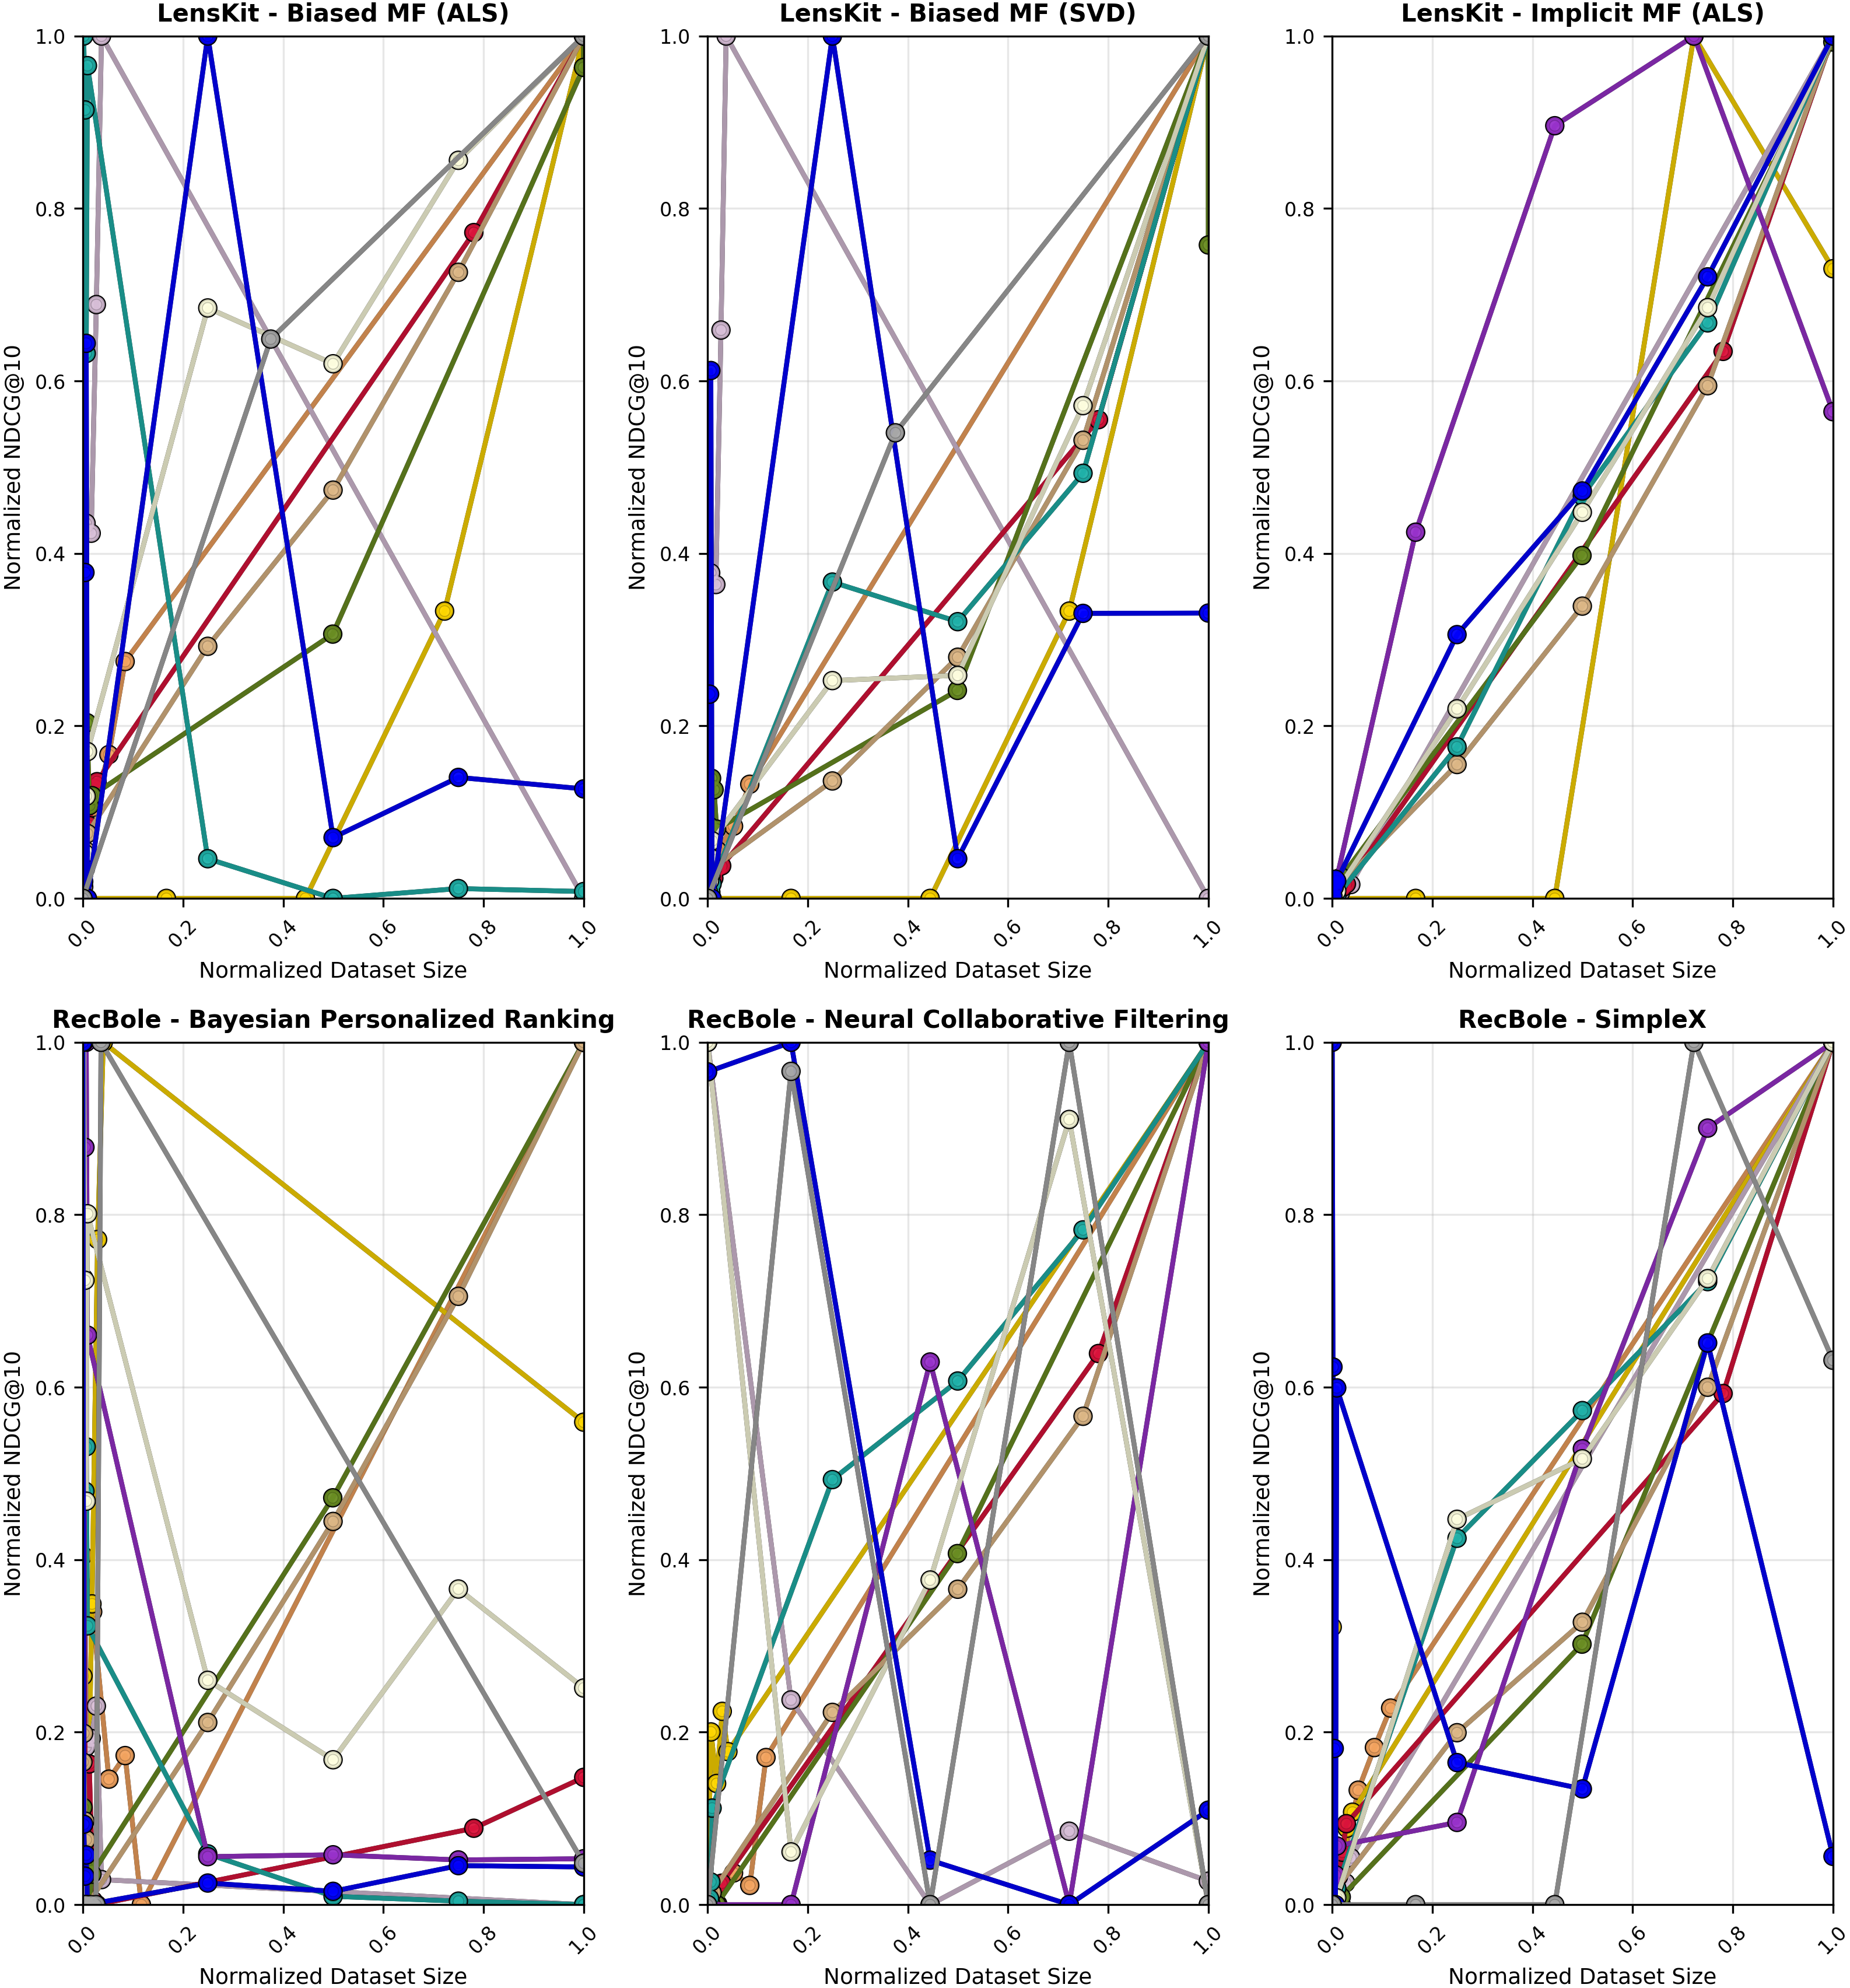
\includegraphics[width=\textwidth]{images/normalized-distinct.png}
    \caption{Min--max normalized version of Figure~\ref{fig:lines-distinct}. Both sample size and $NDCG@10$ are normalized within each group.}
    \label{fig:normalized-distinct}
\end{figure}

Figures~\ref{fig:normalized-common} and \ref{fig:normalized-distinct} make the trajectory shapes much easier to compare across diverse datasets. In the Popularity panels, the dominant pattern is close to an ideal positive scaling path: groups tend to begin near $(0,0)$ and end near $(1,1)$, so the largest relative sample size often coincides with the group's best relative $NDCG$. At the opposite extreme, the RecBole BPR panel contains many groups whose final point at $x=1$ does not lie at $y=1$, so the largest available sample does not produce the group's peak performance. The normalized view also makes several weaker deviations more interpretable, particularly for Last.fm, TMall, and Amazon. Amazon becomes more visually prominent in the normalized figures even though its raw coverage is limited; this is analytically useful, but it must be interpreted with caution because normalization magnifies short or incomplete trajectories as strongly as fully observed ones. Despite these caveats, the normalized line plots again show that many groups follow a broadly positive relationship between relative size and relative performance.

\subsubsection{Scatter by Dataset}
\begin{figure}[H]
    \centering
    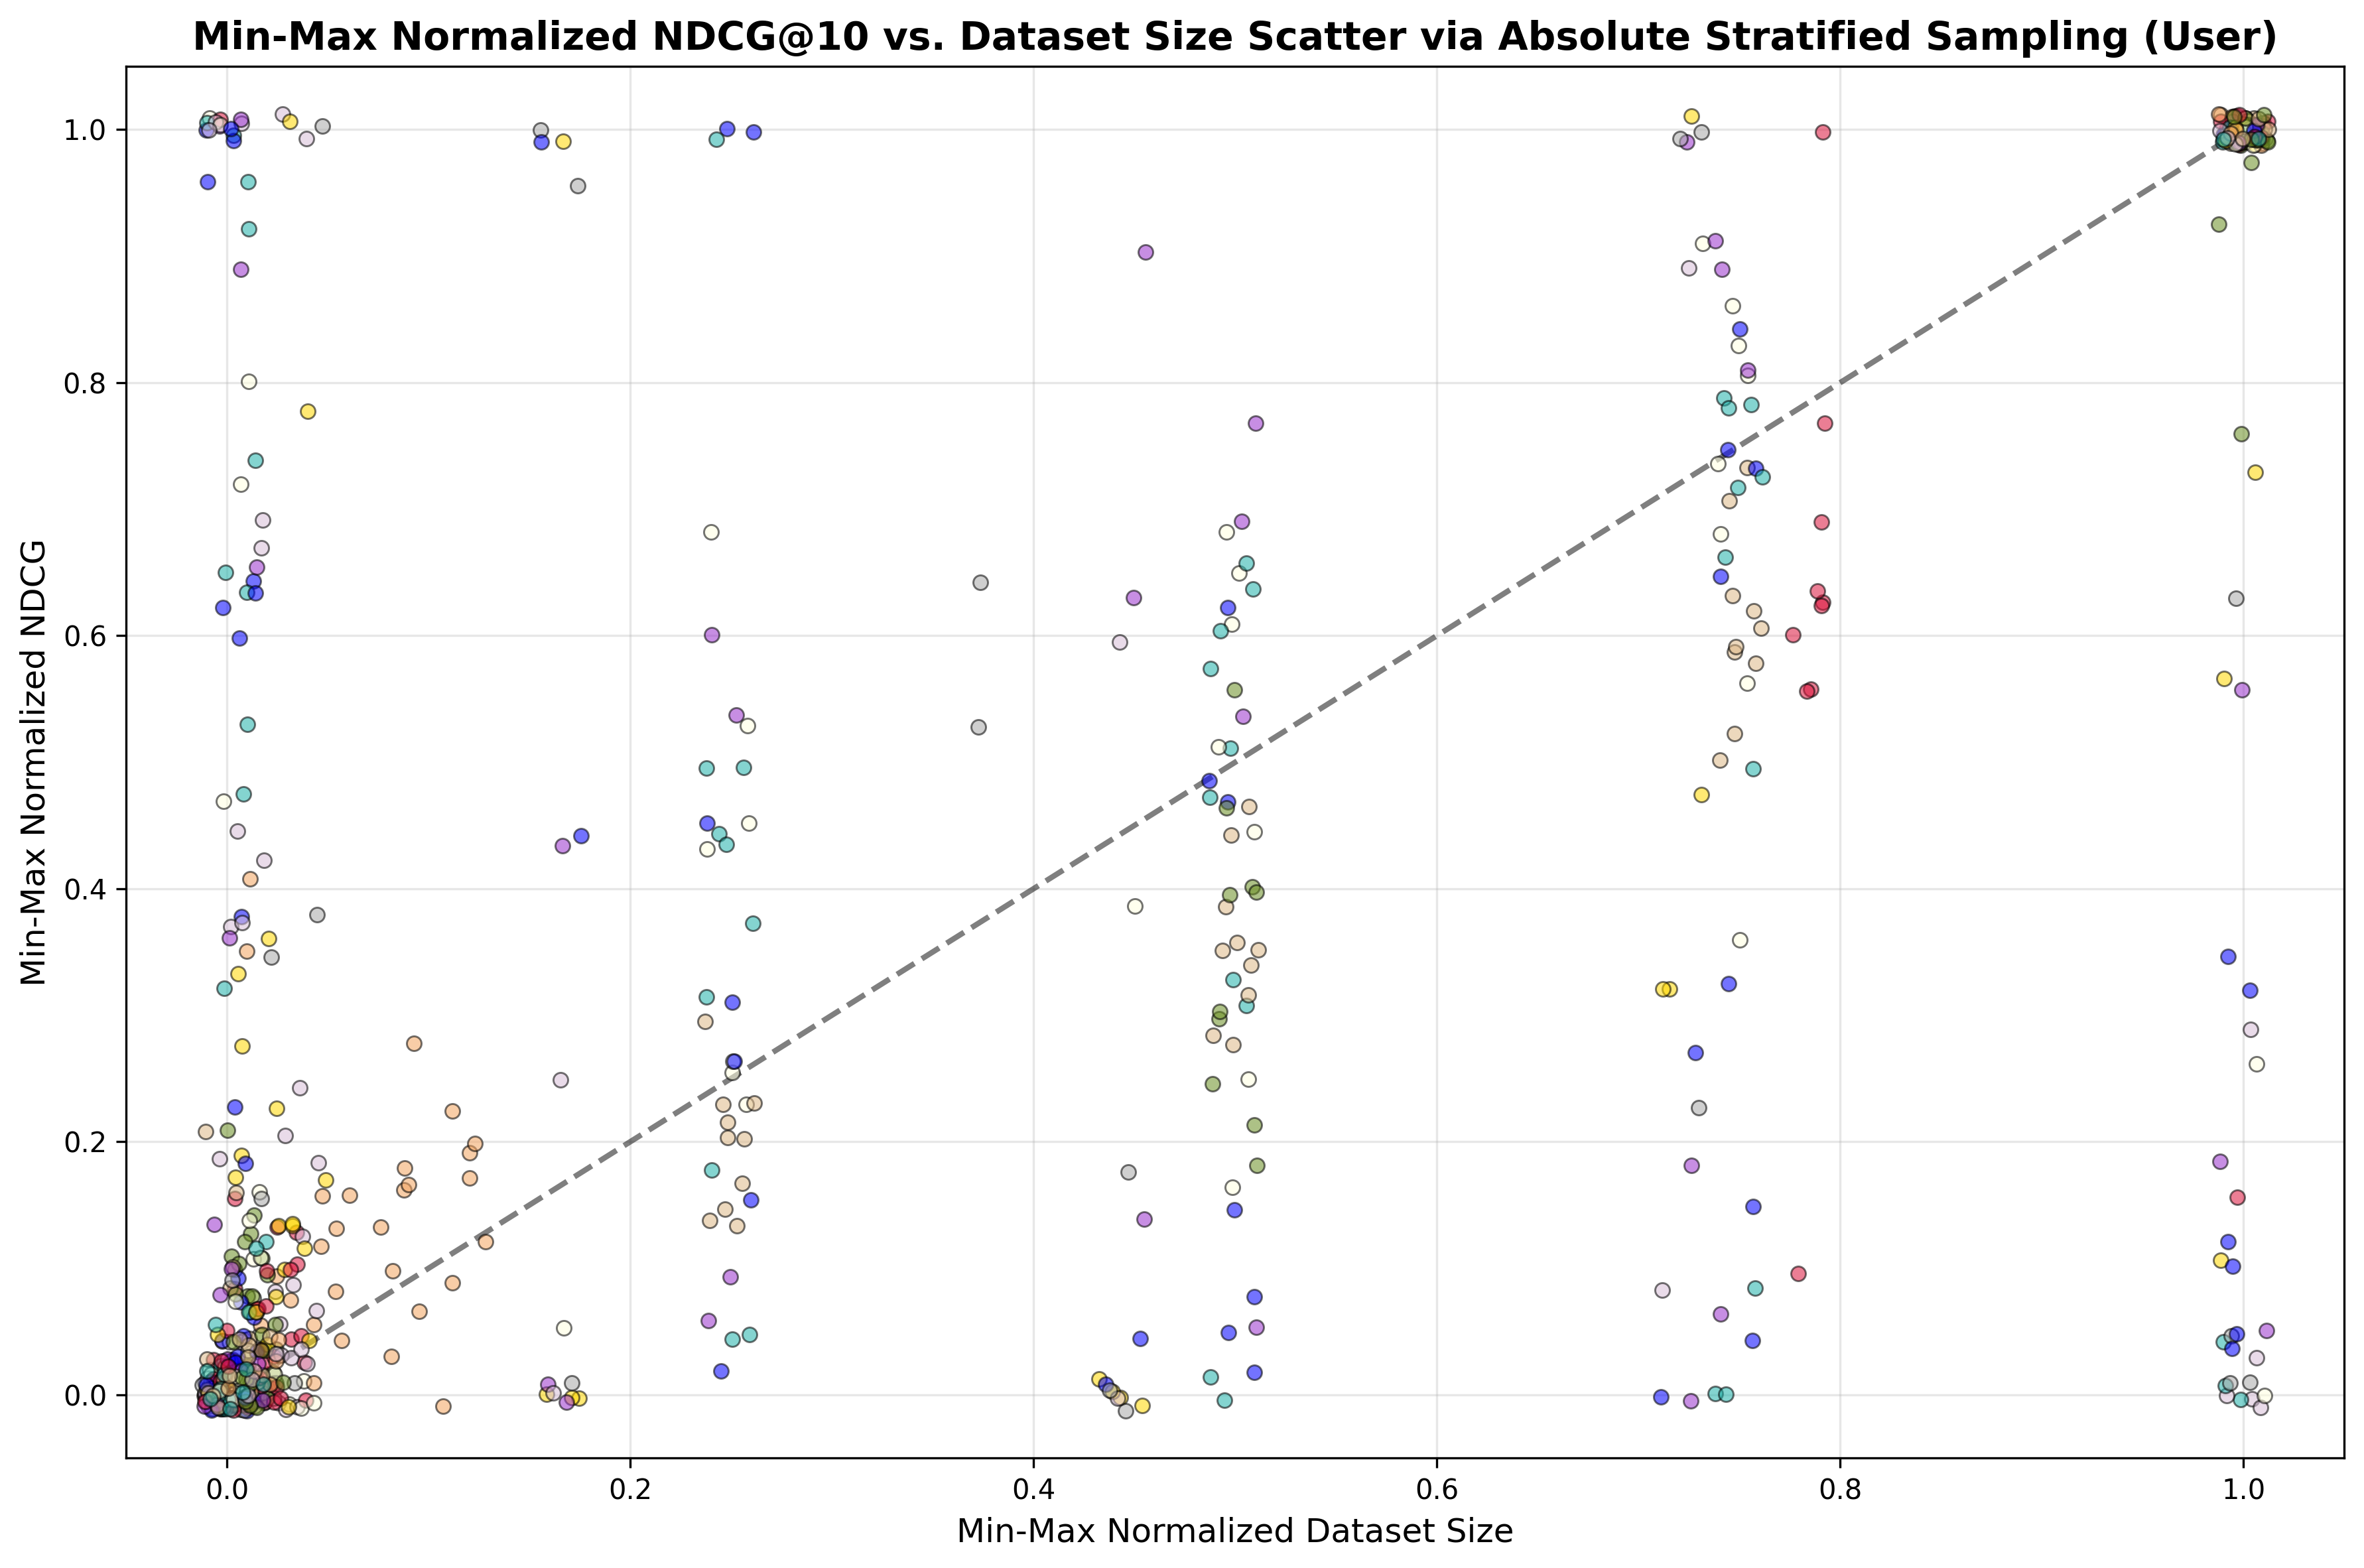
\includegraphics[width=\textwidth]{images/scatter-datasets.png}
    \caption{Scatter plot of all normalized instances, colored by dataset. The dashed diagonal indicates the reference line $y=x$.}
    \label{fig:scatter-datasets}
\end{figure}

Figure~\ref{fig:scatter-datasets} combines all normalized instances into a single scatter plot and colors them by dataset. The dashed diagonal from $(0,0)$ to $(1,1)$ serves as a visual reference for an idealized linear relationship between relative size and relative performance. A small random jitter in both axes was added purely for readability so that dense overlaps at points such as $(0,0)$ and $(1,1)$ remain visible. The dominant pattern is a concentration of points near both endpoints of the diagonal, with more diffuse clouds around intermediate positions such as approximately $(0.25,0.25)$, $(0.5,0.5)$, and $(0.75,0.75)$. This indicates that many groups begin at their within-group minimum, end at or near their within-group maximum, and vary mainly in the path taken between those two extremes. When attention is restricted to visible outliers, the greatest deviations from the diagonal appear to occur more often in Last.fm, Amazon, Alibaba-iFashion, and a subset of Yahoo Music points. Even so, the overall distribution remains broadly consistent with the positive scaling trends already visible in the line plots.

\subsubsection{Scatter by Tool--Algorithm Pair}
\begin{figure}[H]
    \centering
    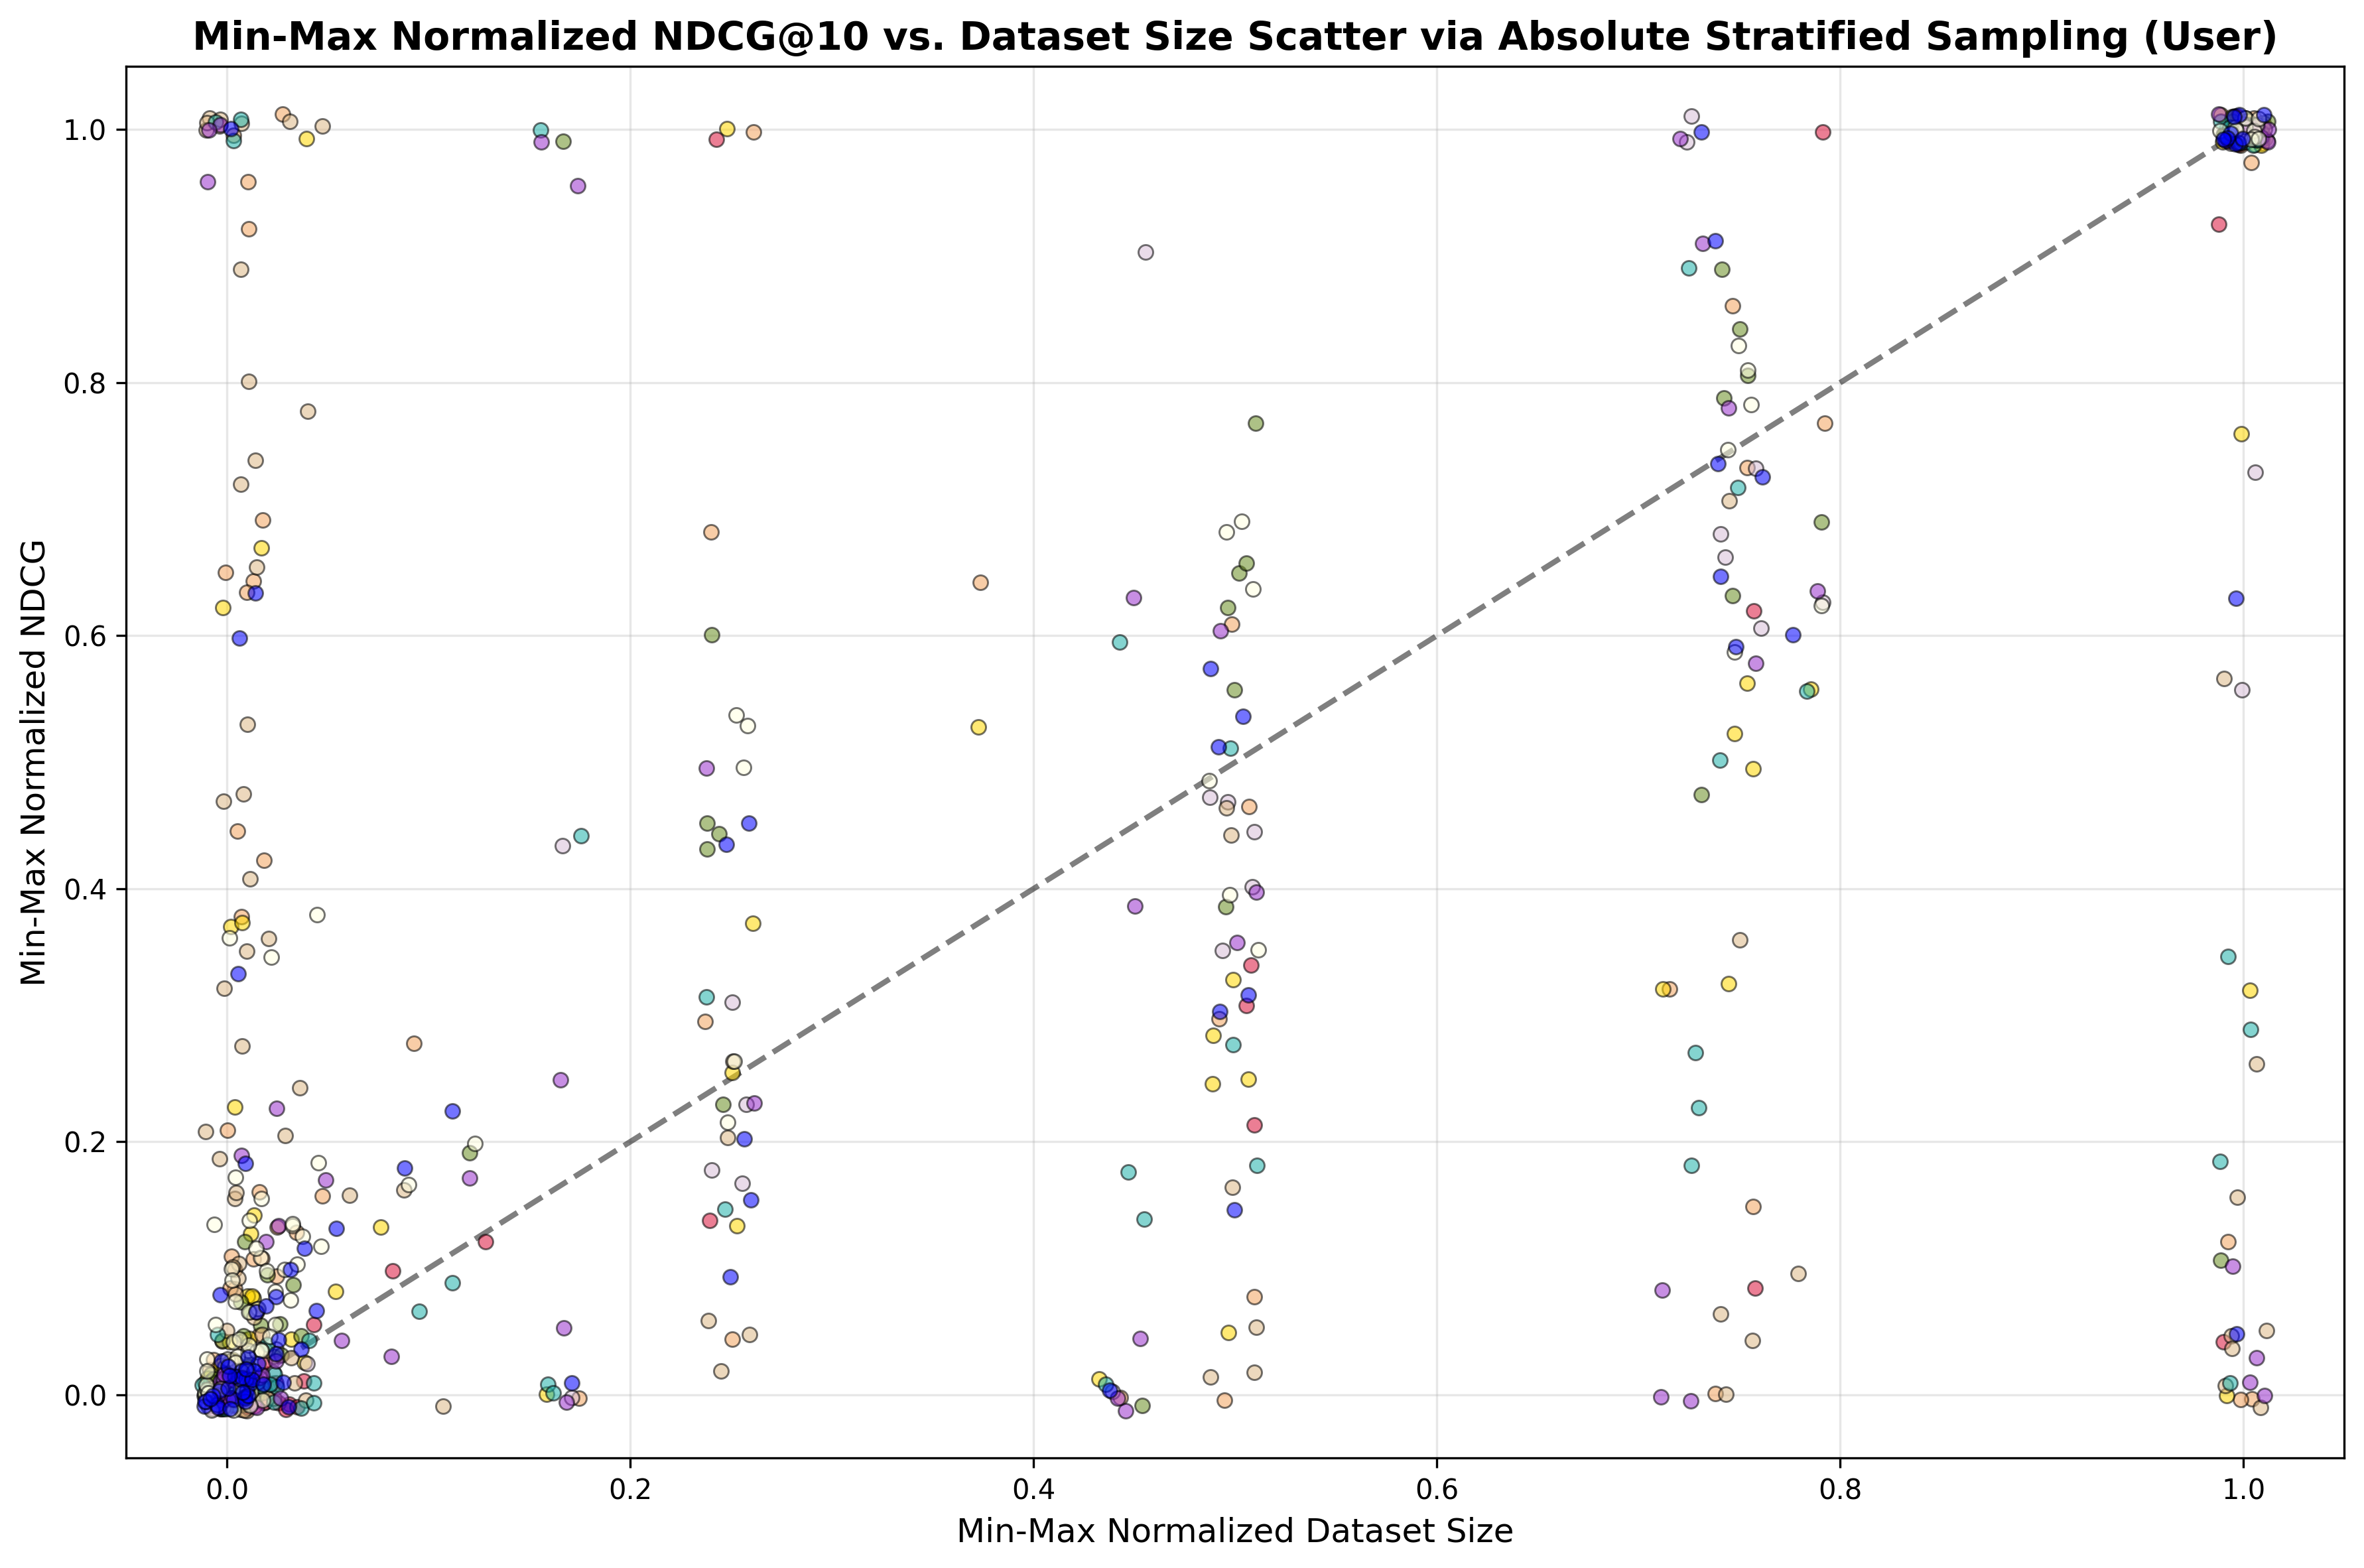
\includegraphics[width=\textwidth]{images/scatter-algorithms.png}
    \caption{Scatter plot of all normalized instances, colored by tool--algorithm pair. The dashed diagonal indicates the reference line $y=x$.}
    \label{fig:scatter-algorithms}
\end{figure}

Figure~\ref{fig:scatter-algorithms} presents the same normalized scatter distribution as Figure~\ref{fig:scatter-datasets}, but recolors the points by tool--algorithm pair according to the legend in Figure~\ref{fig:legend-algorithms}. The identical jitter used in both figures enables direct visual comparison between the dataset-colored and algorithm-colored views, so that the same point can be interpreted simultaneously in terms of dataset identity and method identity. This makes the source of prominent outliers easier to diagnose. In particular, a substantial share of the visibly dispersed or off-diagonal points is associated with RecBole BPR, which is consistent with the poor scaling behavior already observed for that method in the preceding raw and normalized analyses.

\subsubsection{Scatter Summary}
\begin{figure}[H]
    \centering
    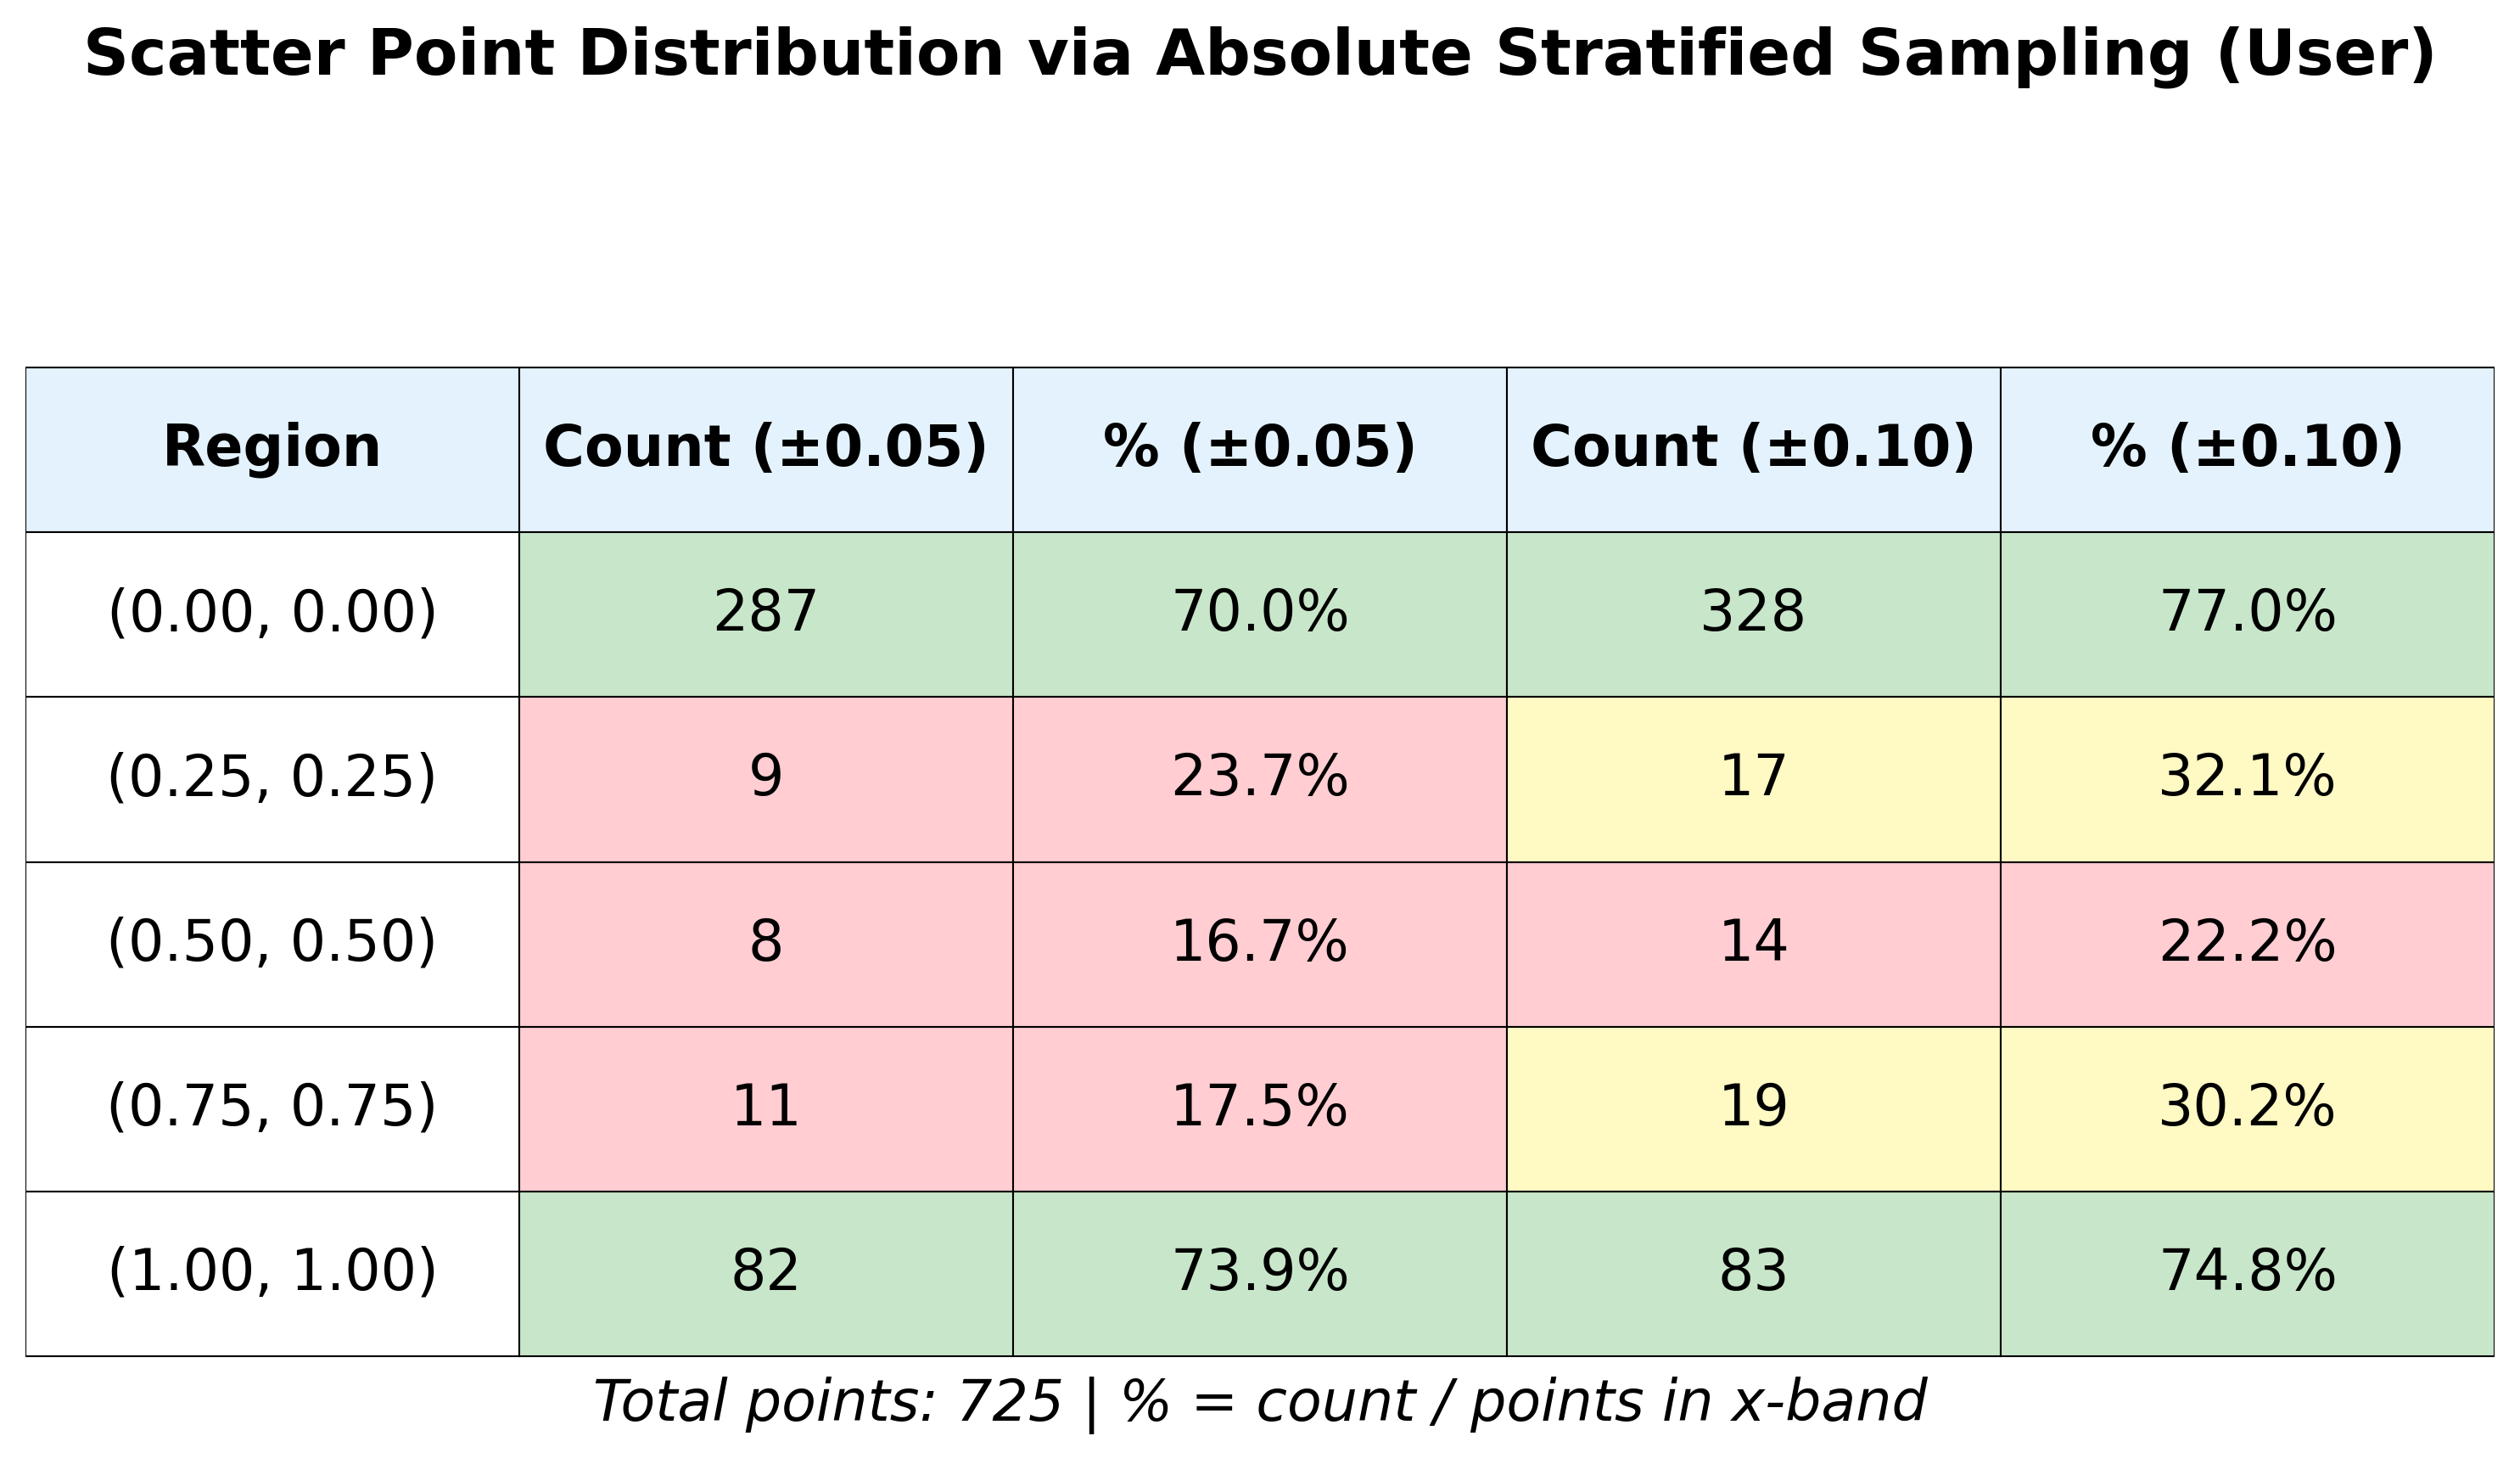
\includegraphics[width=\textwidth]{images/scatter-metadata.png}
    \caption{Summary table of normalized-point concentrations around selected diagonal reference locations.}
    \label{fig:scatter-metadata}
\end{figure}

Figure~\ref{fig:scatter-metadata} summarizes the concentration of normalized points around selected locations along the diagonal reference line used in the scatter plots. For each region, the table reports both counts and percentages under two tolerance levels, namely $\pm 0.05$ and $\pm 0.1$. This tabular view makes the visual impression from Figures~\ref{fig:scatter-datasets} and \ref{fig:scatter-algorithms} easier to verify. In particular, the strongest concentrations occur near the endpoints $(0,0)$ and $(1,1)$, where the counts are at least $70\%$ under both tolerances, indicating that many groups begin close to their minimum relative performance and finish close to their maximum relative performance. Intermediate regions are more dispersed, but even there the table still suggests non-random clustering around the diagonal. Taken together, the scatter plots and metadata summary show that clustering near the diagonal remains common in the normalized results.

\subsection{Late-Stage Slopes}
This subsection summarizes the final visible segment of each normalized group by means of the late-stage slope defined above. Intuitively, this quantity captures the ``last rise'' before the largest available sample size. Groups with fewer than five instances were excluded from this analysis because a reliable late-stage segment cannot be defined for very short trajectories. If the slopes were concentrated near zero, that would be suggestive of systematic saturation. Conversely, a predominance of positive slopes indicates that, even near the end of the observed size range, additional data often continues to improve recommendation quality.

\subsubsection{By Dataset}
\begin{figure}[H]
    \centering
    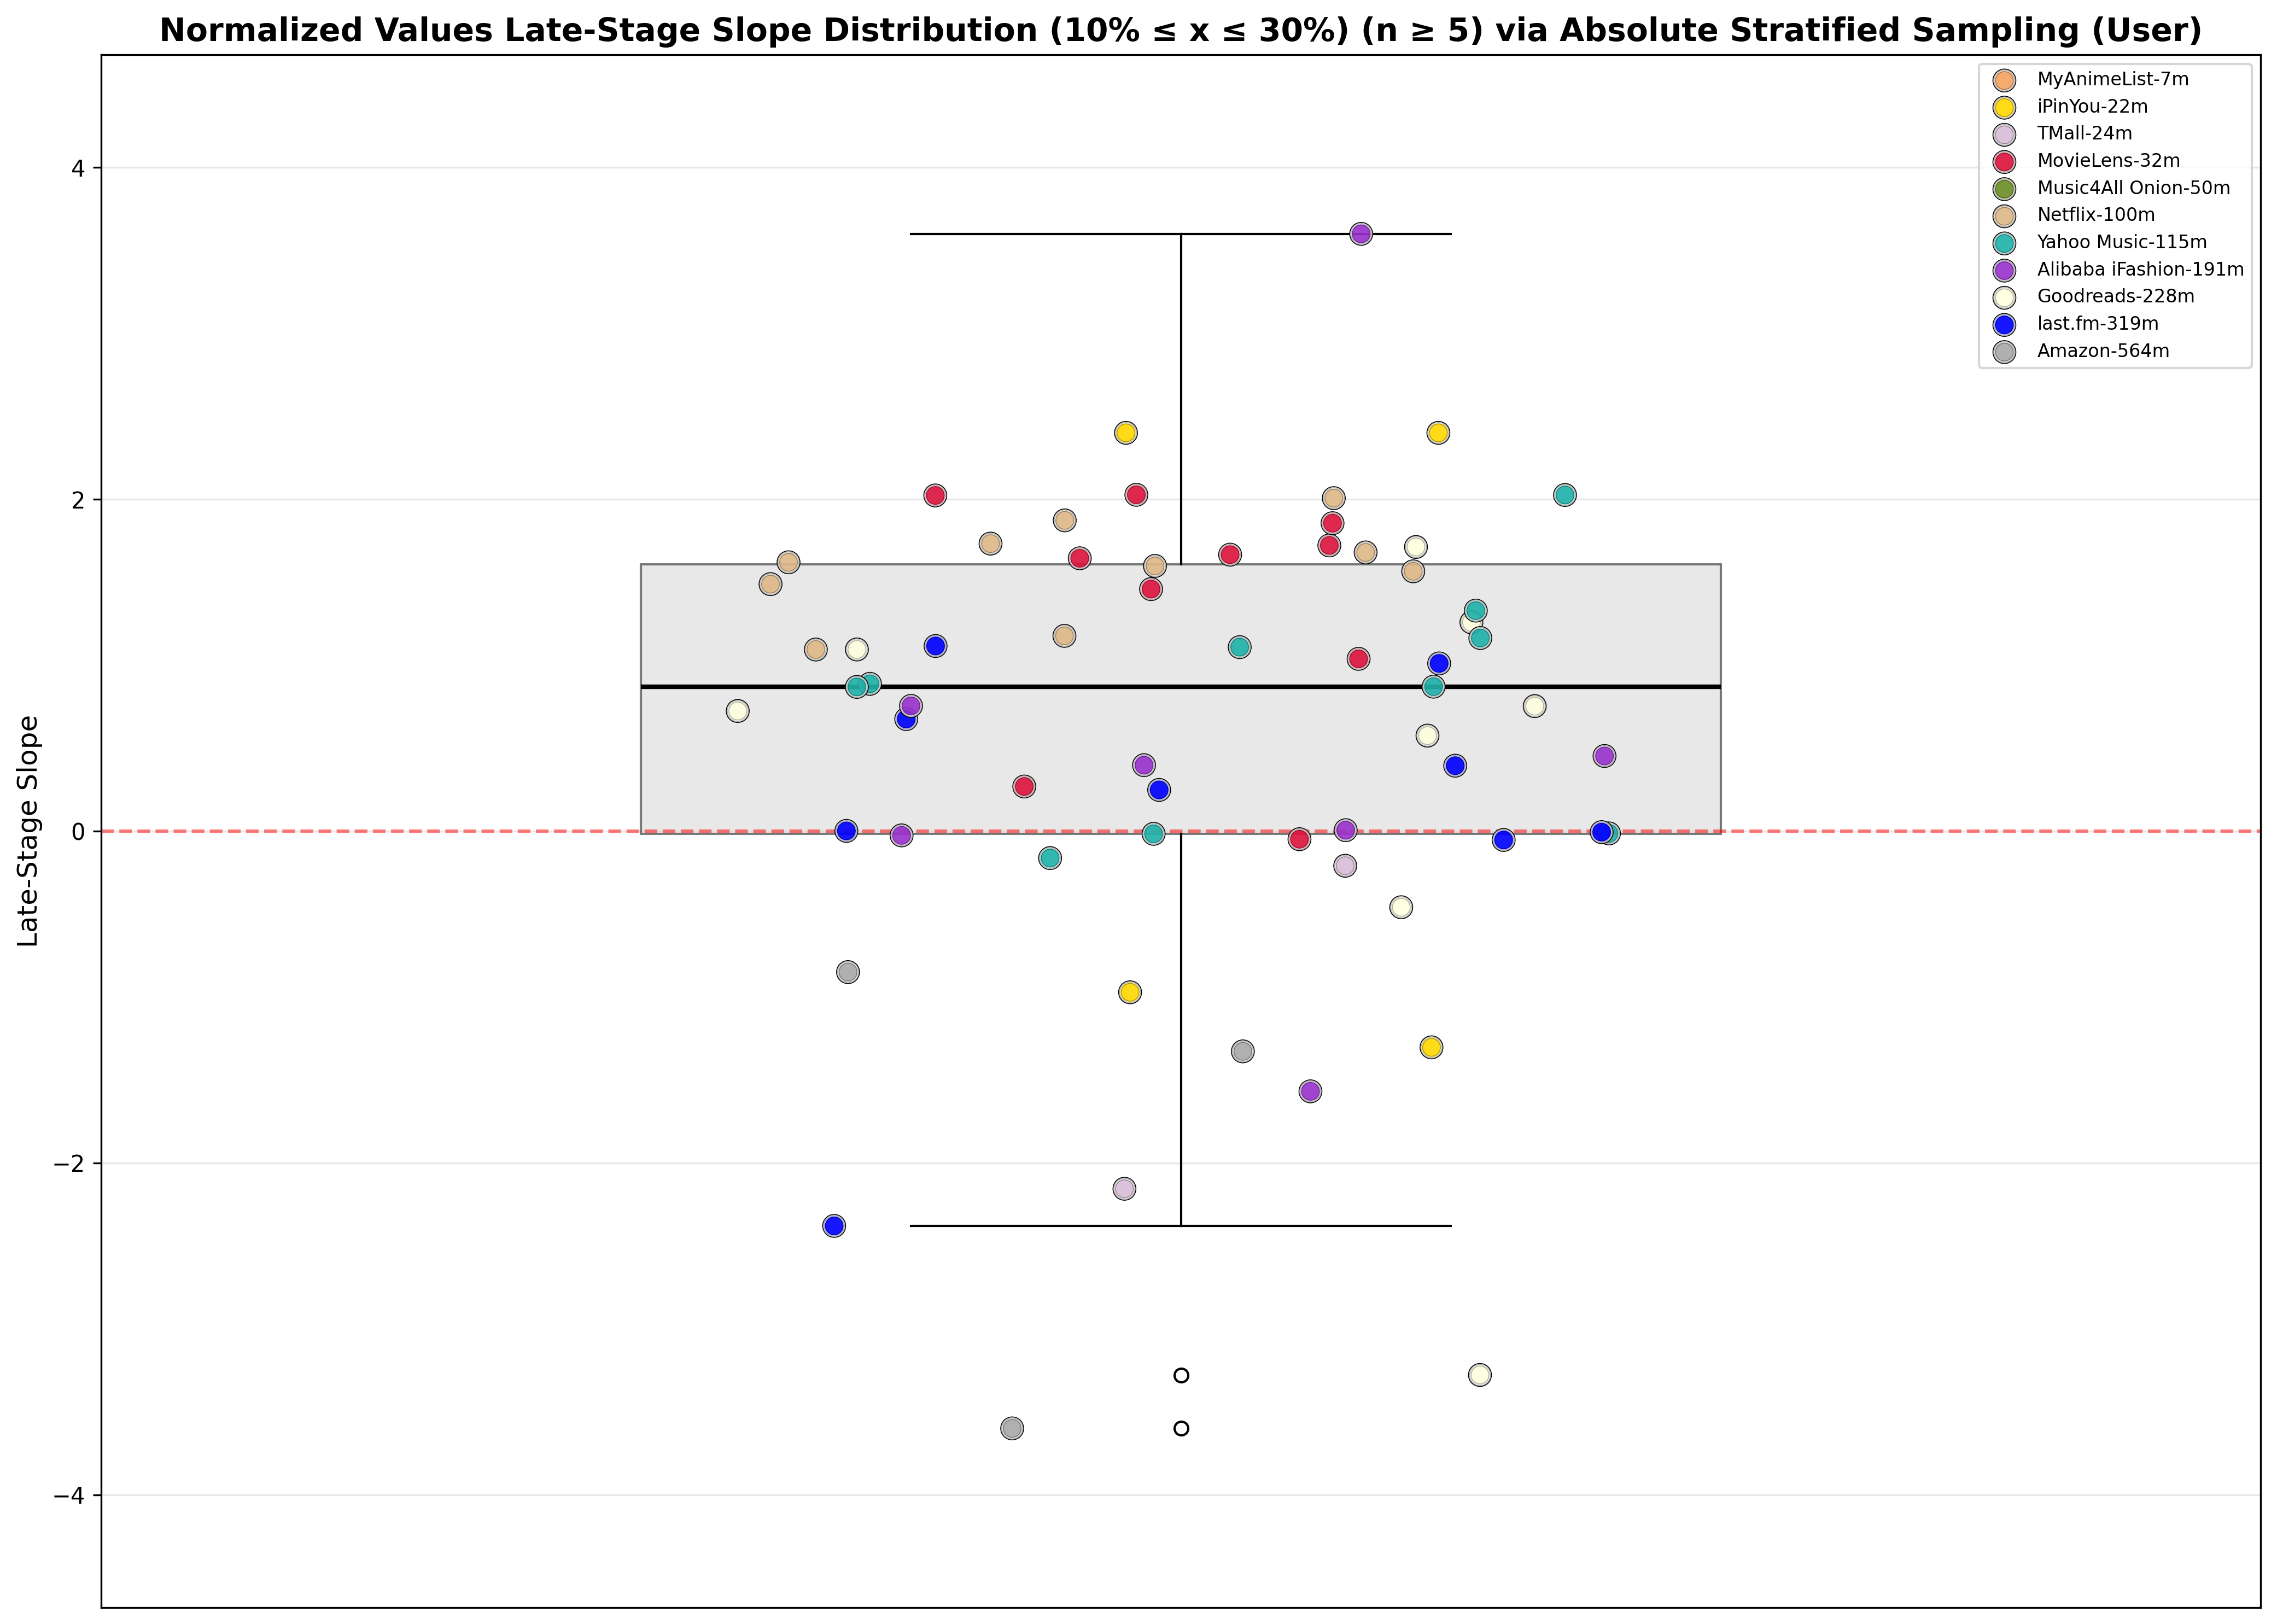
\includegraphics[width=\textwidth]{images/slopes-datasets.png}
    \caption{Distribution of late-stage slopes, with points colored by dataset. Horizontal jitter is used only to reduce overlap.}
    \label{fig:slopes-datasets}
\end{figure}

Figure~\ref{fig:slopes-datasets} shows that the late-stage slope distribution is centered on positive values rather than around zero. The interquartile range extends from approximately $0$ to $1.5$, with a mean slightly below $1$, while the whiskers span roughly from $-2.25$ to $3.5$. The final observed segment of most eligible groups is therefore non-negative and often distinctly positive. In the dataset-colored view, many points from Netflix, MovieLens, Yahoo Music, and Goodreads occupy the interquartile region and the upper half of the distribution, whereas the more negative tail is visually associated more often with Amazon. Although individual negative outliers remain present, the overall distribution remains weighted toward non-negative slopes.

\subsubsection{By Tool--Algorithm Pair}
\begin{figure}[H]
    \centering
    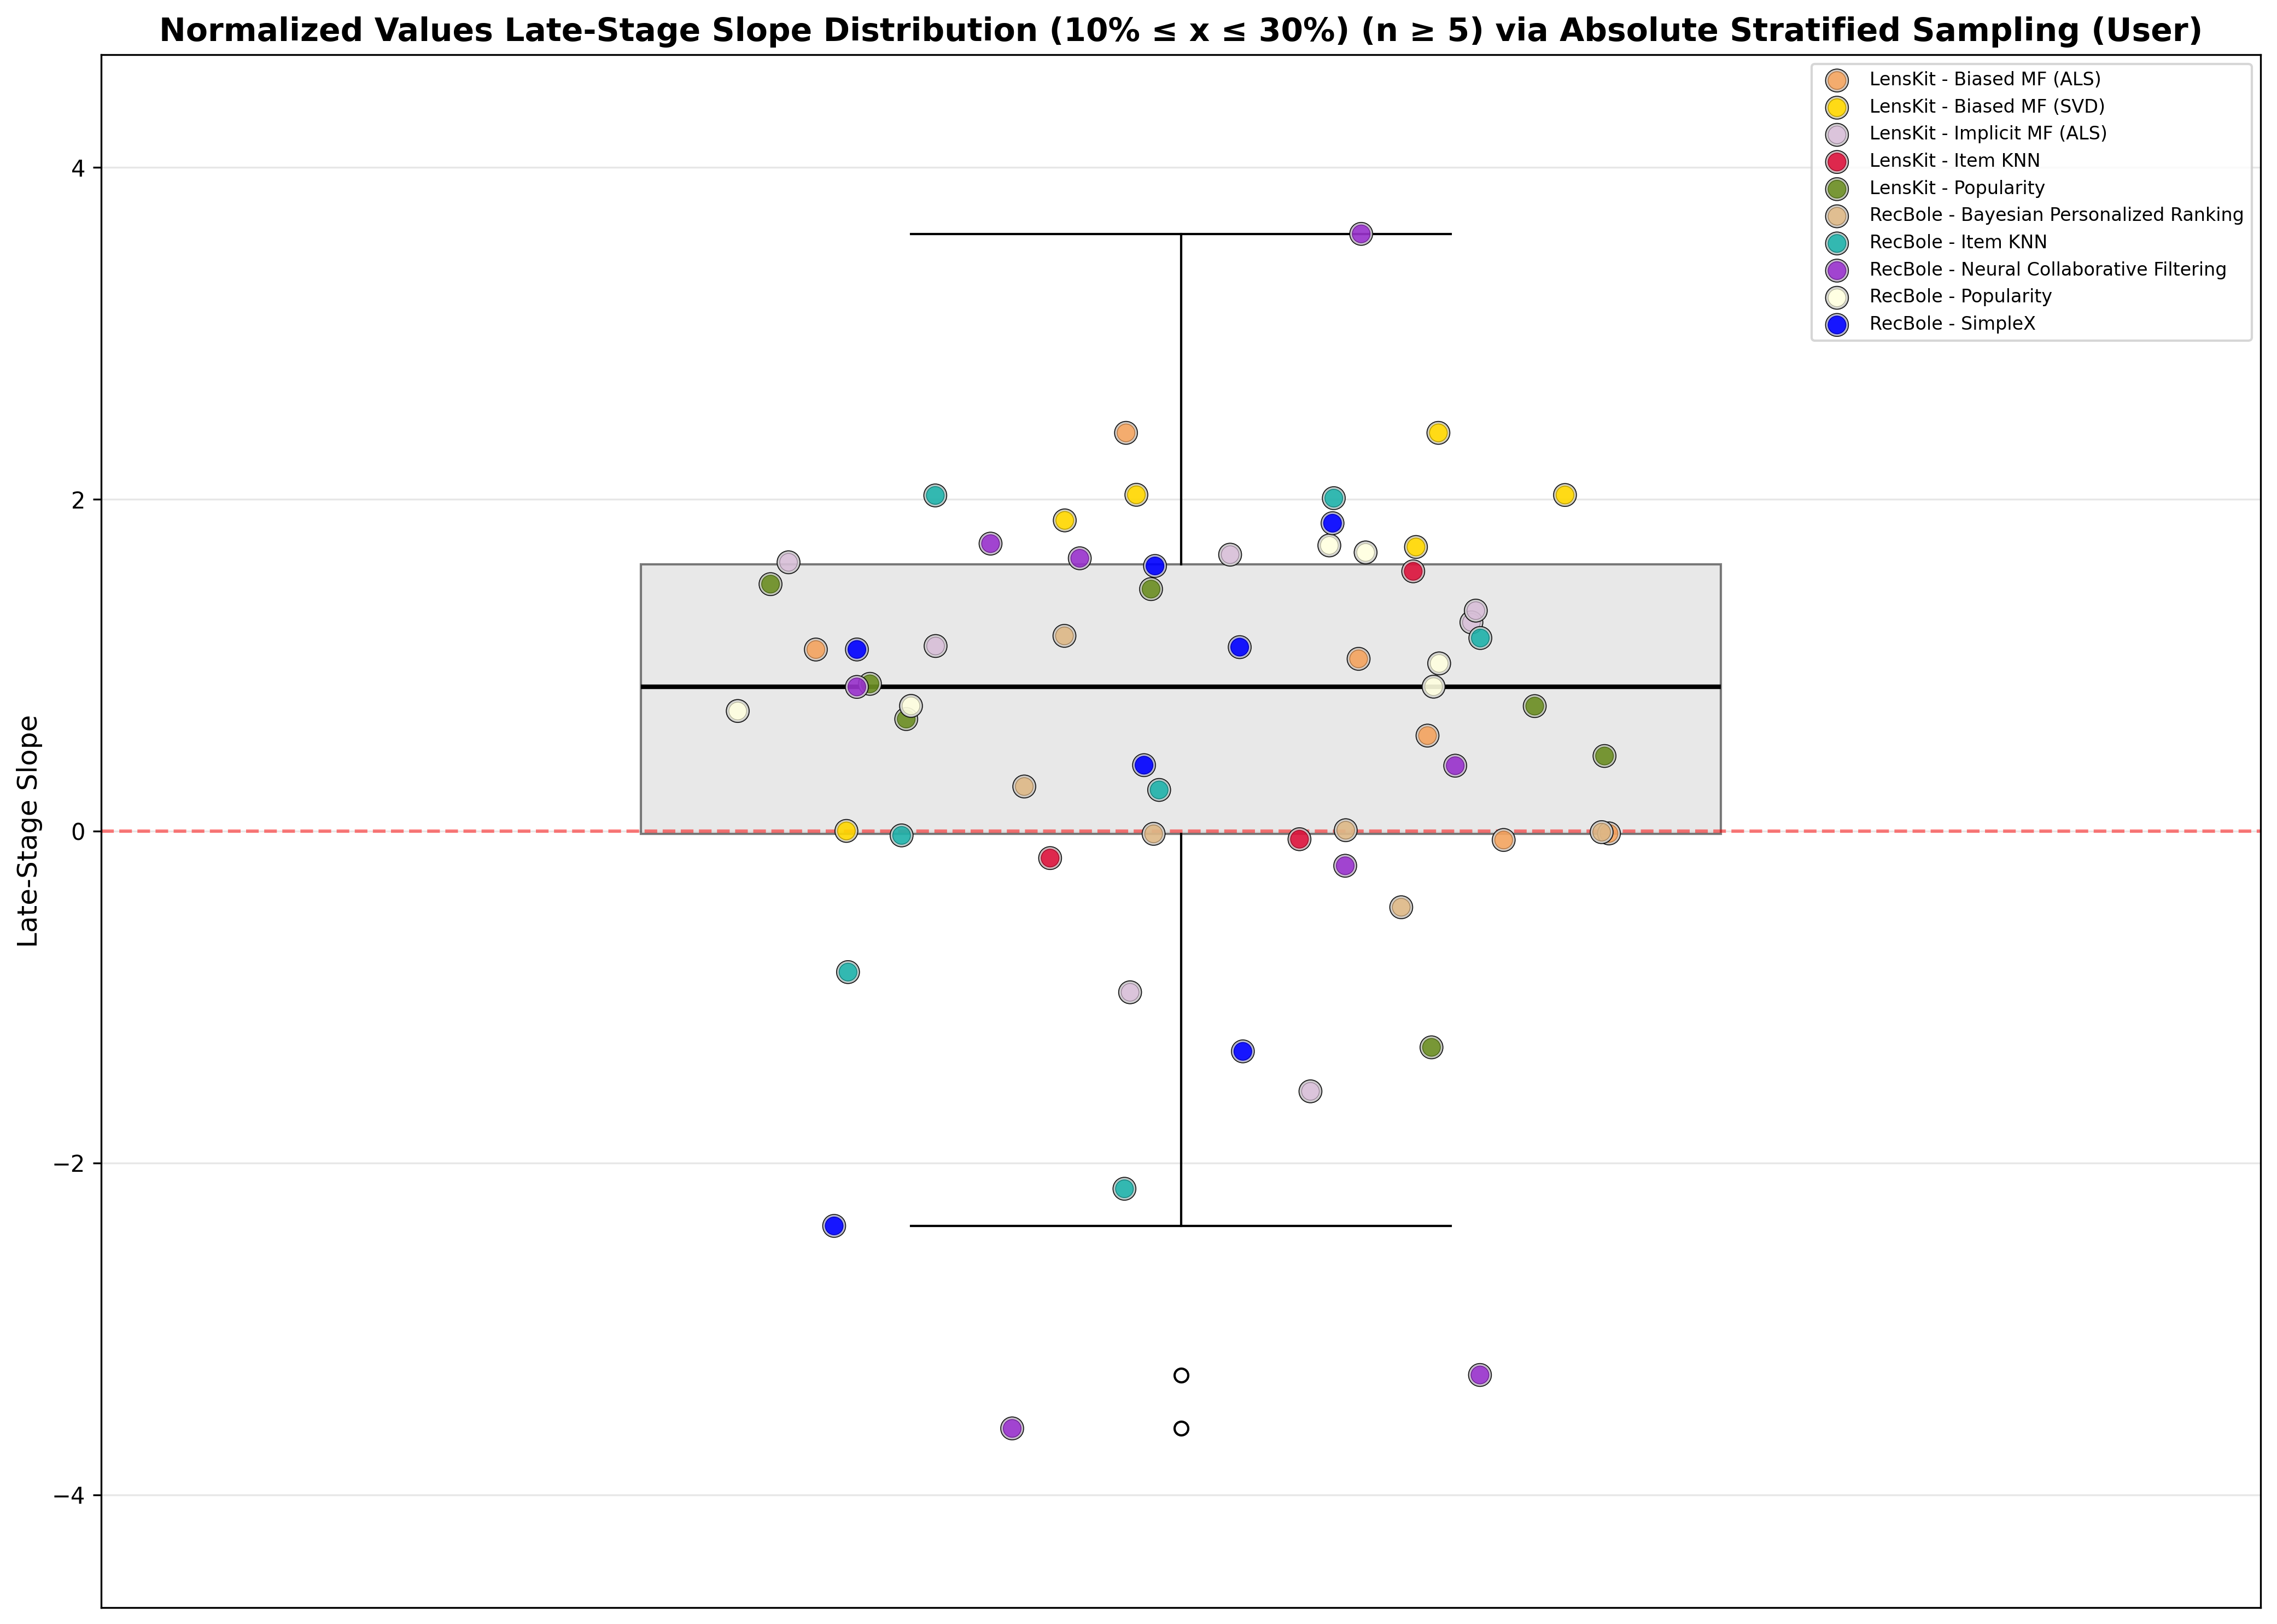
\includegraphics[width=\textwidth]{images/slopes-algorithms.png}
    \caption{Distribution of late-stage slopes, with points colored by tool--algorithm pair. Horizontal jitter is used only to reduce overlap.}
    \label{fig:slopes-algorithms}
\end{figure}

Figure~\ref{fig:slopes-algorithms} preserves the same slope distribution but recolors the points by tool--algorithm pair. This makes it possible to identify which methods contribute most strongly to the positive and negative ends of the distribution. Positive late-stage slopes are visibly common for both Popularity baselines, and they are also well represented among LensKit BiasedSVD, LensKit ImplicitMF, RecBole SimpleX, and RecBole NeuMF. By contrast, the lower tail does not appear to be dominated exclusively by RecBole BPR: many BPR values hover near the $0$ mark rather than populating the most negative region. Instead, several of the more negative slopes are distributed across a smaller number of RecBole ItemKNN and NeuMF groups, especially when combined with weaker-performing datasets such as TMall or Amazon. Overall, the negative cases appear concentrated in a limited subset of model--dataset combinations.

\subsection{Summary Tables}
The following tables condense the figure-level observations into dataset-by-algorithm summaries. In each table, rows correspond to datasets and columns correspond to tool--algorithm combinations. Colored cells indicate whether the reported value supports a strong positive scaling interpretation to a greater or lesser extent, while grey cells indicate that the corresponding group did not satisfy the requirements for inclusion and are therefore left blank. These summaries are useful because they reduce complex trajectories to a small number of interpretable indicators: where the maximum occurs, how early near-maximum performance is reached, and how much additional benefit remains near the upper end of the sample-size range.

\subsubsection{Maxima}
\begin{figure}[H]
    \centering
    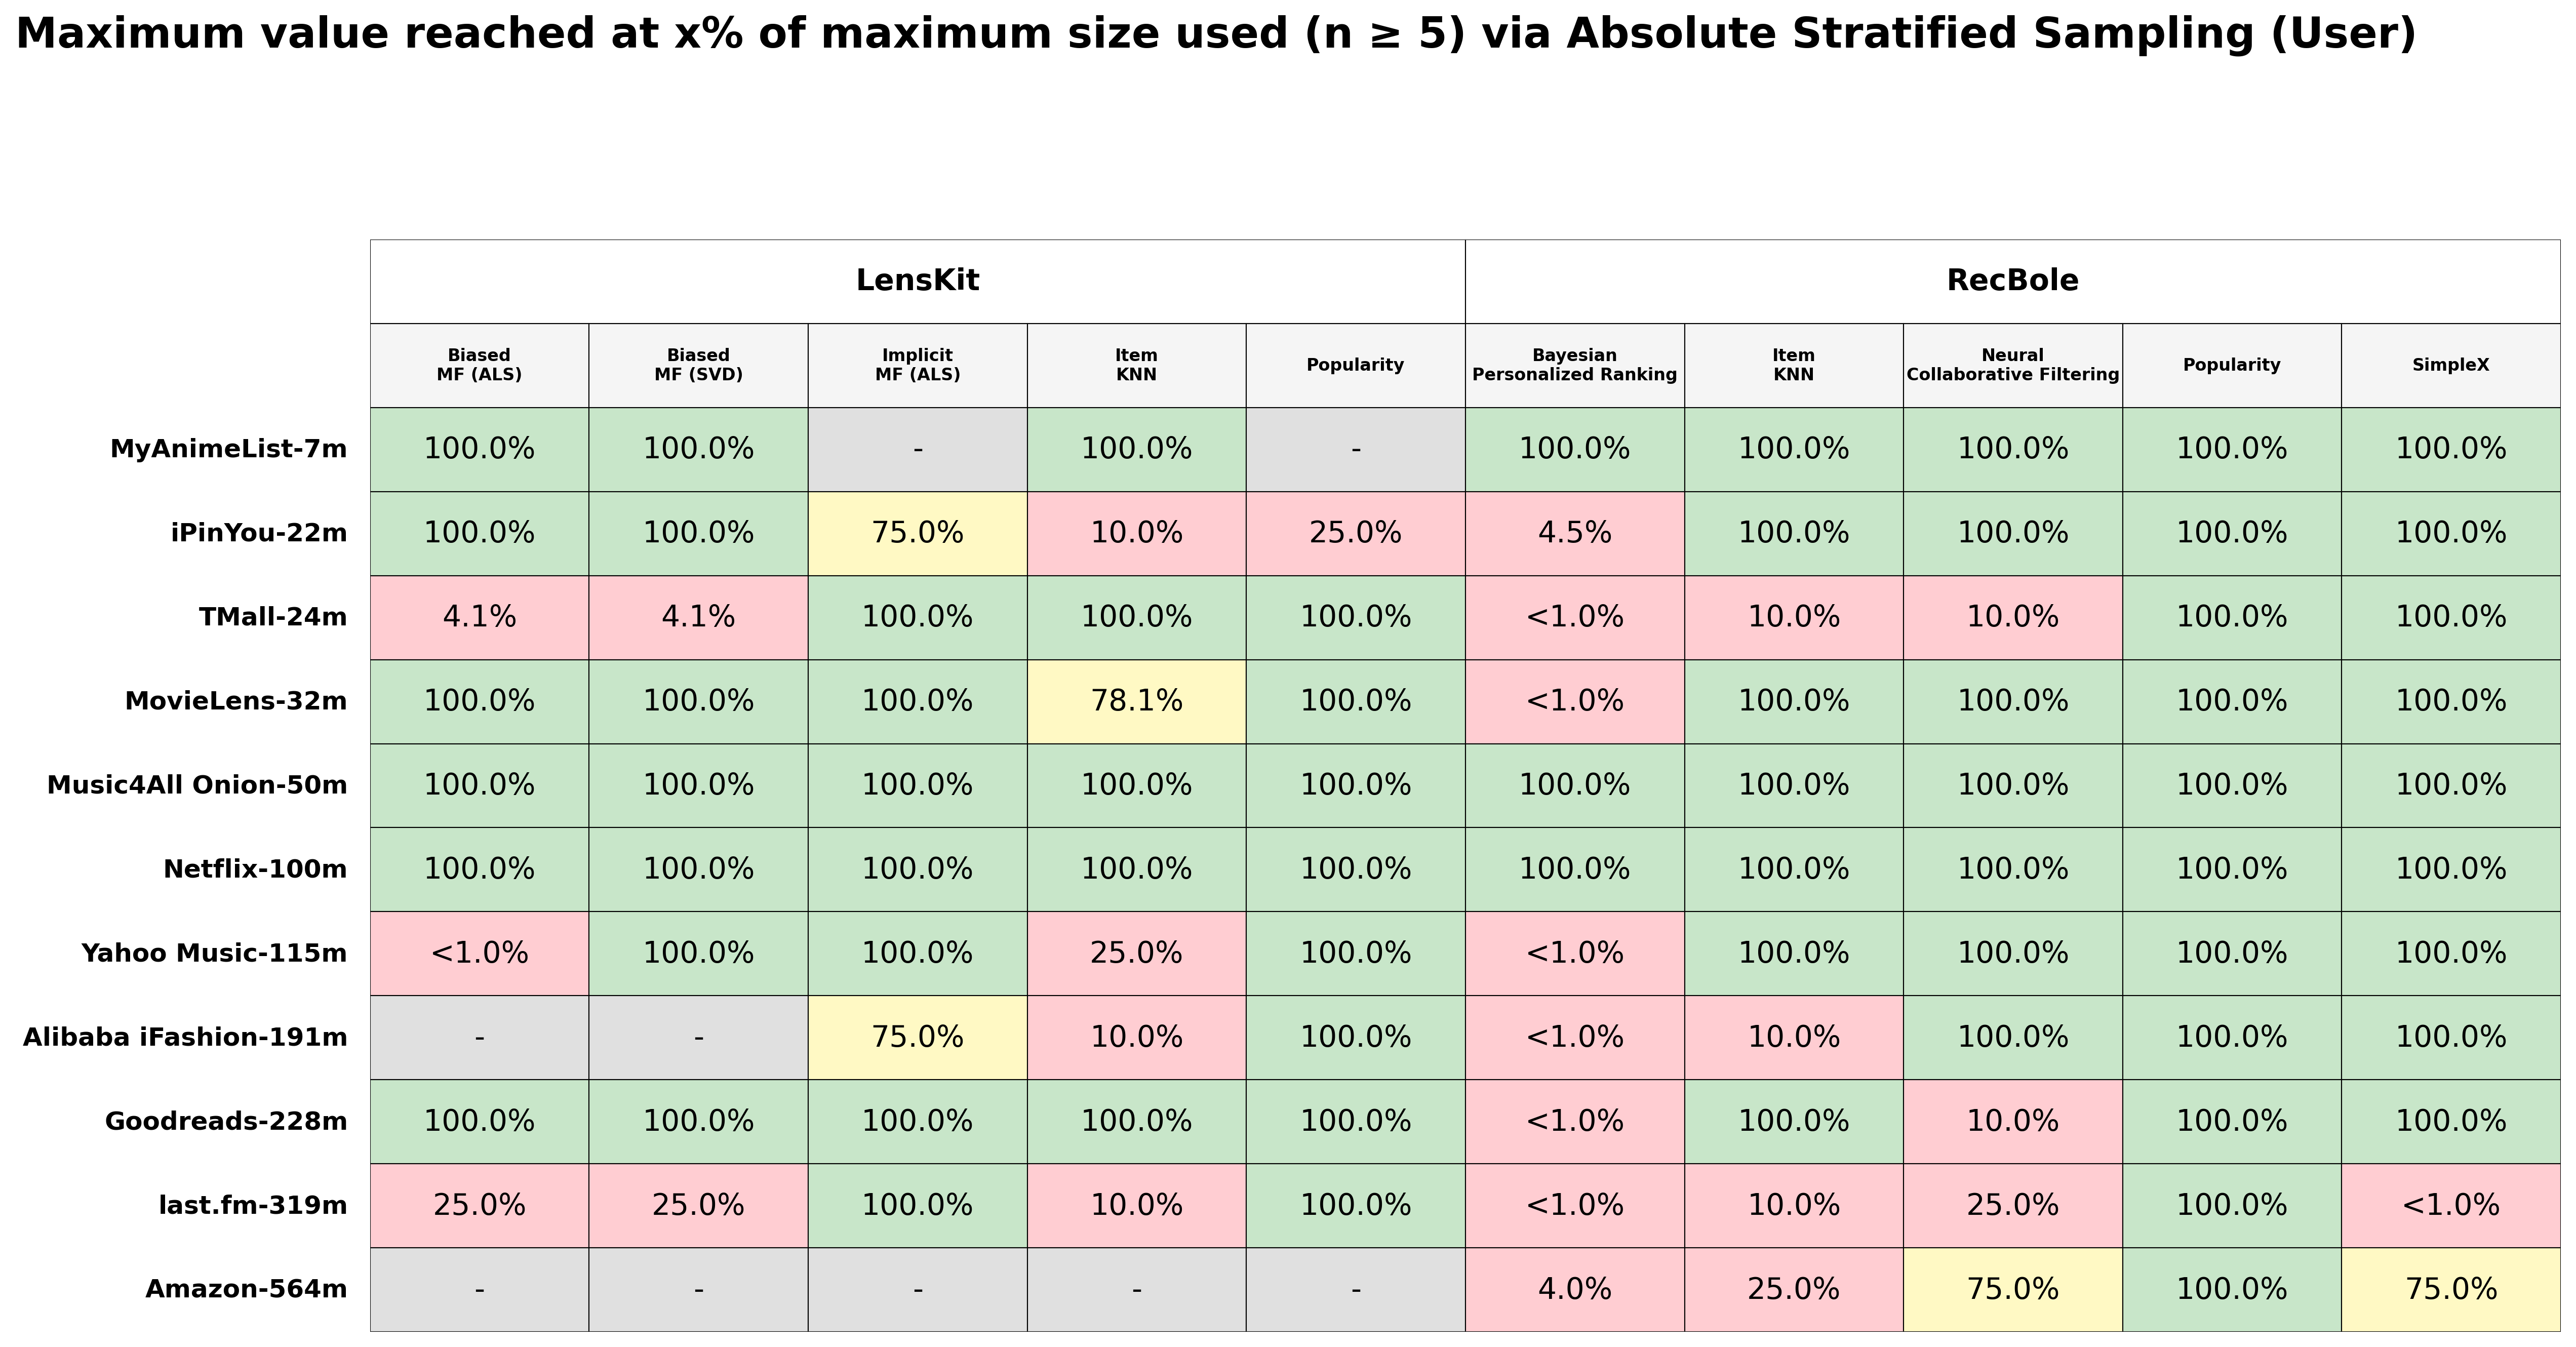
\includegraphics[width=\textwidth]{images/maxima.png}
    \caption{Percentage of the largest completed sample size at which each eligible group attains its maximum observed $NDCG@10$.}
    \label{fig:maxima}
\end{figure}

Figure~\ref{fig:maxima} reports, for each eligible group, the relative sample size at which the maximum observed $NDCG$ occurs. The most striking pattern is the prevalence of $100\%$ entries, indicating that the best observed performance is most often achieved at the largest completed sample size. This table therefore gives a compact and direct summary of the broader visual trend already seen in the line plots. The small number of low-valued cells correspond to groups whose highest performance occurred very early and was never surpassed thereafter; these cases are consistent with the previously identified outliers and appear disproportionately in RecBole BPR and in some Last.fm-based groups. Overall, the maxima table shows that the maximum most often occurs at the largest completed sample size.

\subsubsection{Elbow Points}
\begin{figure}[H]
    \centering
    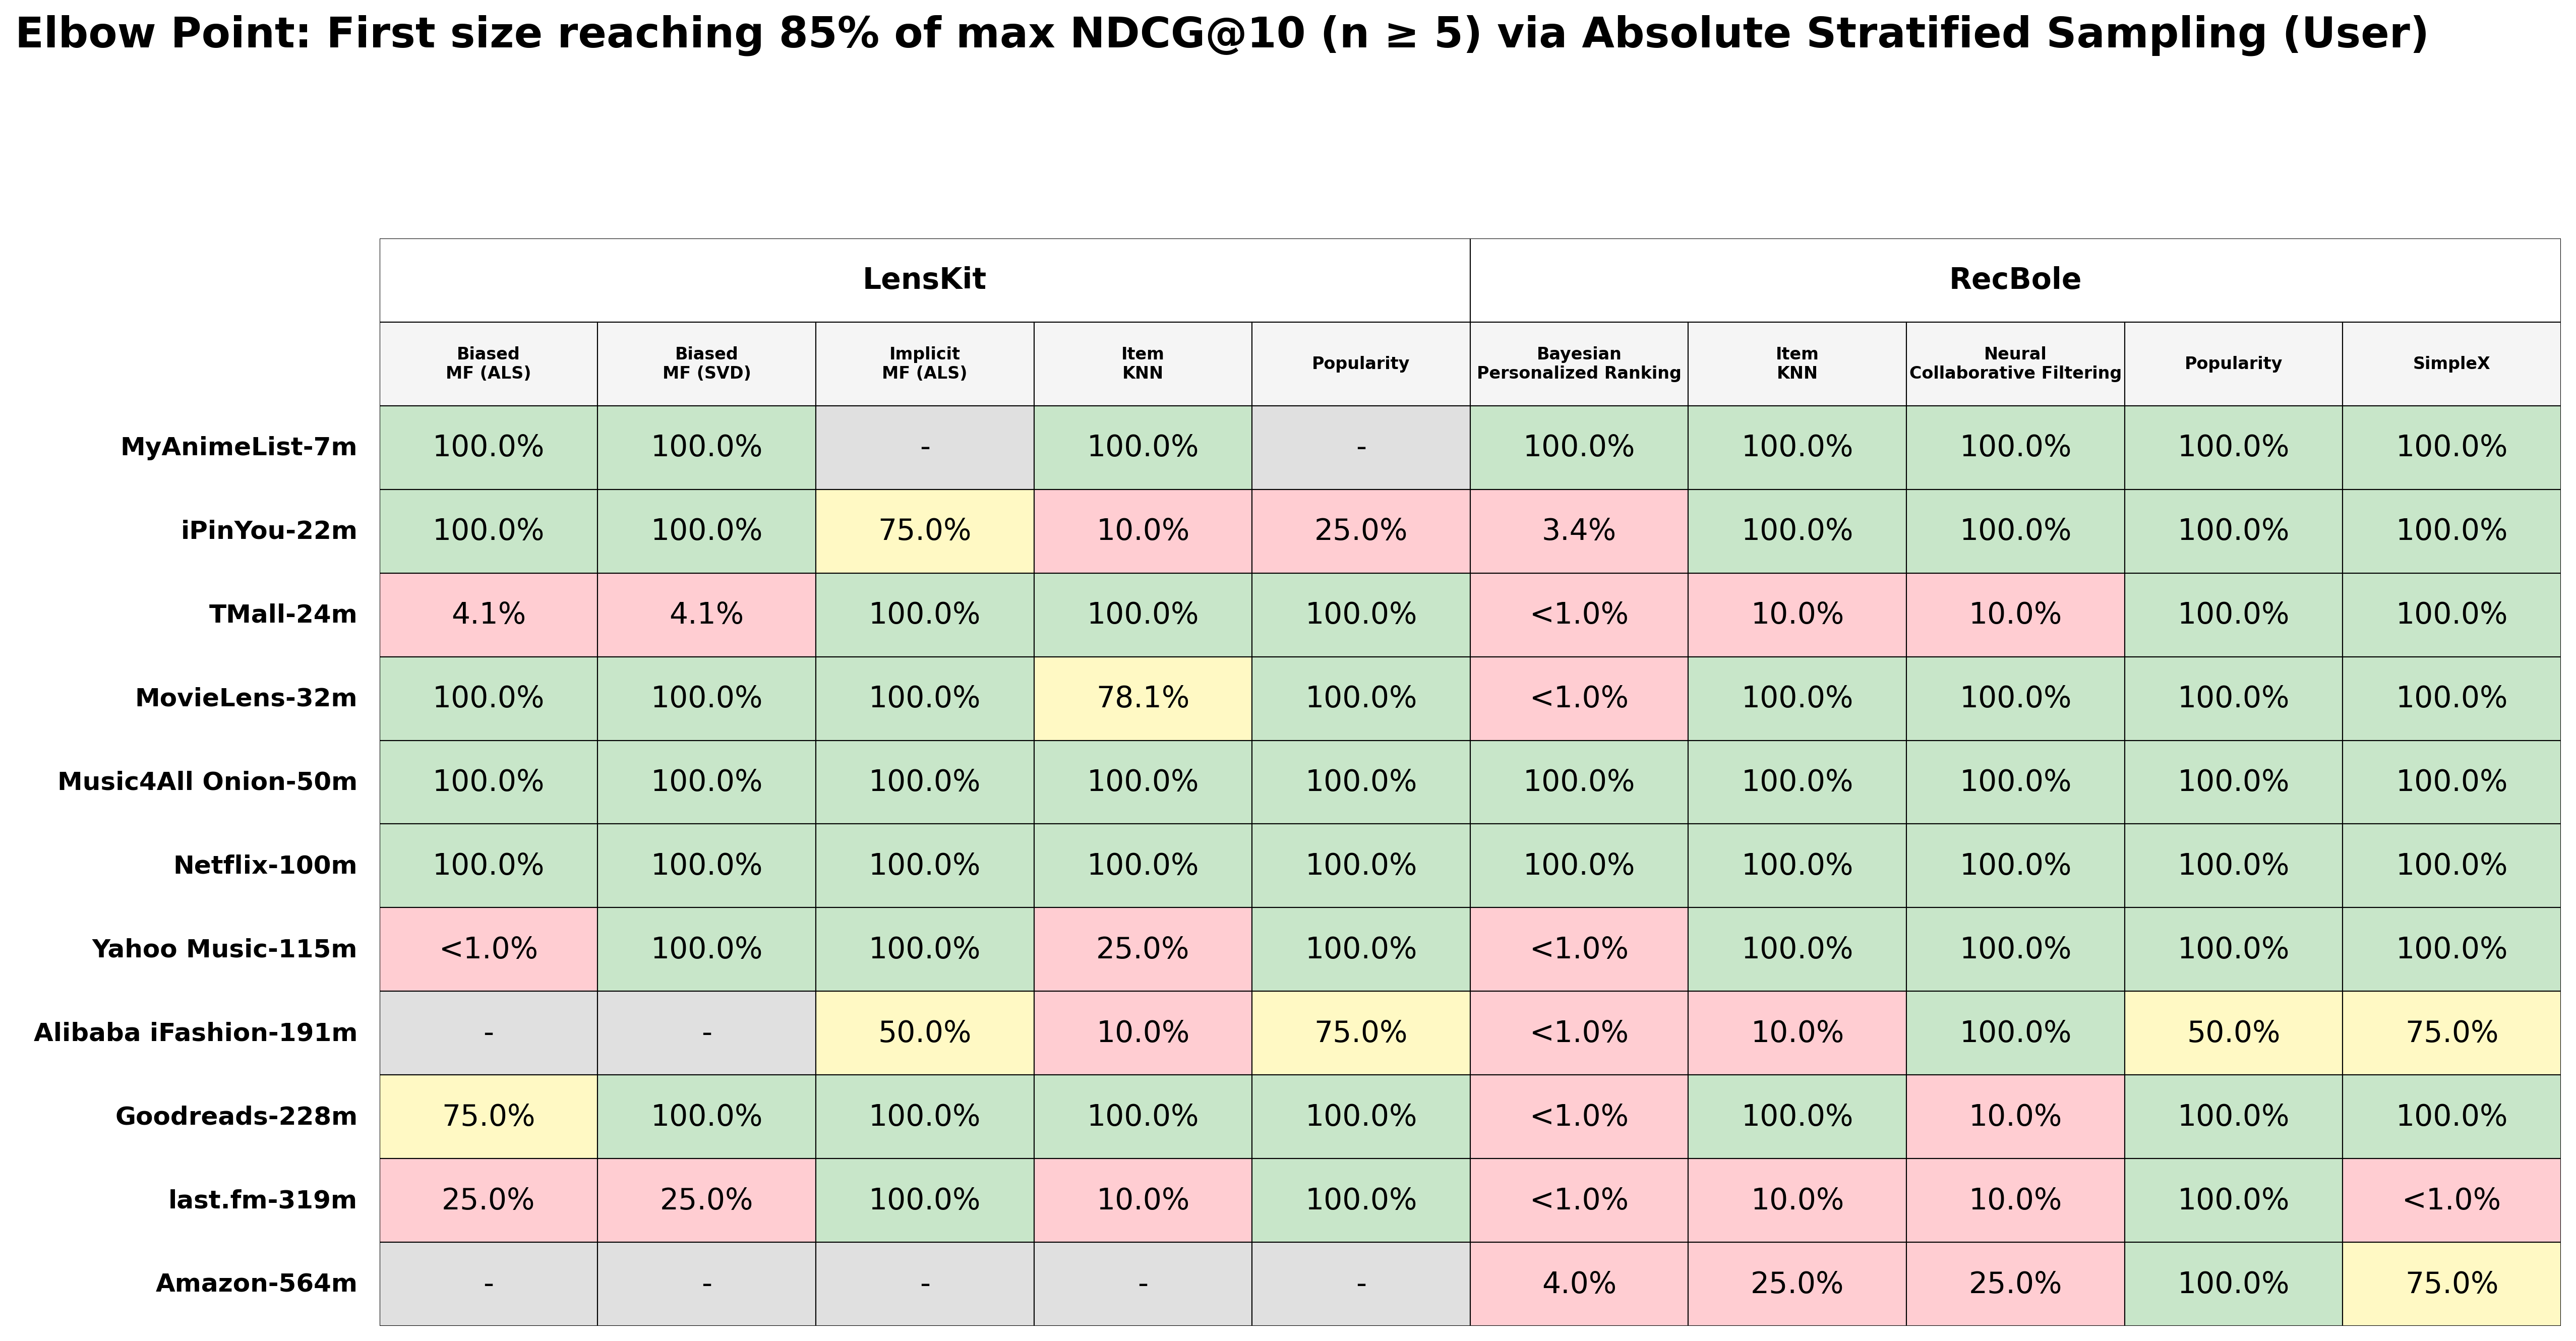
\includegraphics[width=\textwidth]{images/elbow.png}
    \caption{Percentage of the largest completed sample size at which each eligible group first reaches at least $85\%$ of its maximum observed $NDCG@10$.}
    \label{fig:elbow}
\end{figure}

Figure~\ref{fig:elbow} shifts attention from where the absolute maximum occurs to how early a group reaches near-maximum performance, defined here as $85\%$ of the group's maximum observed $NDCG$. This is useful from a practical perspective because it indicates how much of the largest sample is needed to obtain performance that is already close to the best achieved in that group. The overall pattern remains nearly identical to the maxima table: for many groups, the elbow point still lies relatively late, often close to the largest sample size. A limited number of earlier elbow points appear, most visibly in parts of the Alibaba-iFashion row, where LensKit ImplicitMF, LensKit Popularity, RecBole Popularity, and RecBole SimpleX reach near-maximum performance as early as half of the largest completed size. Nevertheless, such cases are exceptions rather than the rule, and most elbow points still occur relatively late in the observed range.

\subsubsection{Gains}
\begin{figure}[H]
    \centering
    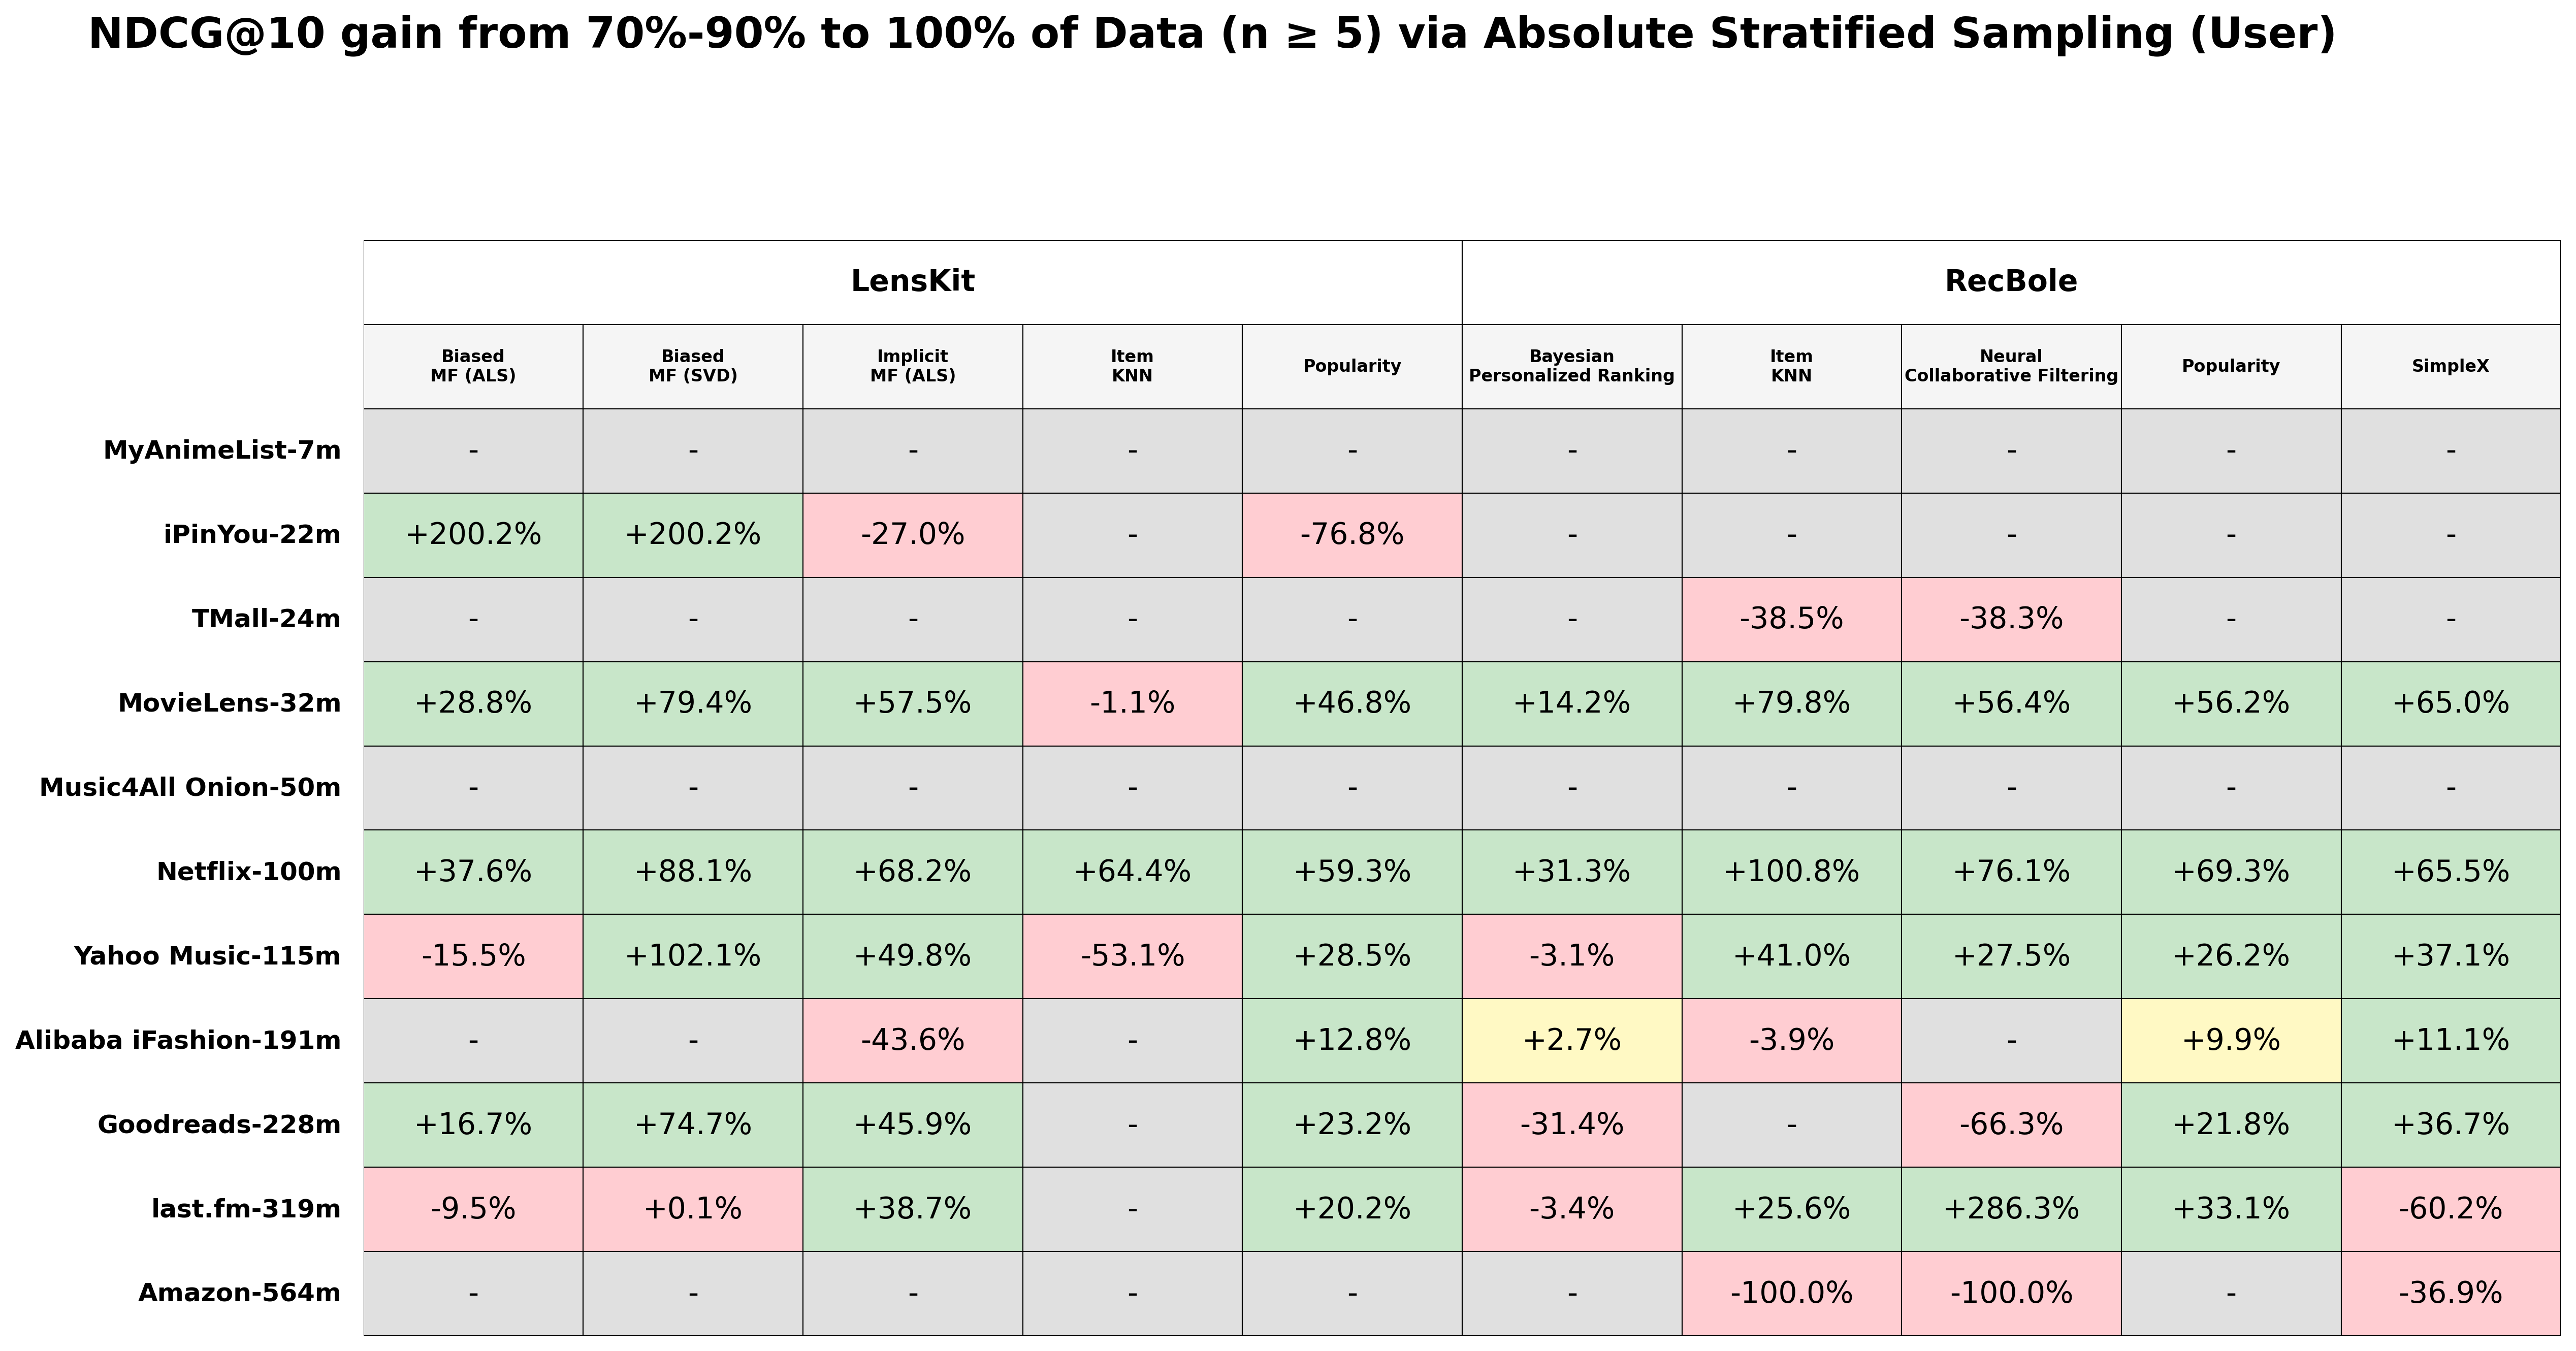
\includegraphics[width=\textwidth]{images/gain.png}
    \caption{Percentage change in $NDCG@10$ from the nearest available sample in the $70\%$--$90\%$ range to the largest completed sample size.}
    \label{fig:gain}
\end{figure}

Figure~\ref{fig:gain} complements the preceding summary tables by quantifying the practical benefit of using all available data rather than only a near-full majority of it. Specifically, it reports the relative change in $NDCG@10$ between the largest completed sample and the nearest available baseline lying within the $70\%$--$90\%$ range of that maximum, with preference given to values closest to the midpoint of the interval. Compared with the maxima and elbow summaries, this table is more sparsely populated because the eligibility criterion is deliberately strict. Under the absolute sizing used in the main experiment, valid comparisons occur primarily for datasets whose largest completed size is at least $100$M, since the immediately preceding size of $75$M falls within the required interval. By contrast, datasets such as Music4All Onion, despite containing many successful runs, often do not provide a suitable near-full baseline under this sizing choice. Broadening the admissible range would increase coverage, but it would also reduce comparability by placing materially different contrasts side by side, for example a $50\%\rightarrow100\%$ comparison next to a $90\%\rightarrow100\%$ comparison. In that sense, a fractional sizing approach would be more favorable for this particular analysis, because it would provide more uniformly comparable near-full reference points across datasets.

Among the cases that do satisfy the criterion, the dominant pattern remains positive and often substantial. Most populated cells indicate gains of at least $10\%$, so the final portion of available data is often associated with a noticeable improvement in ranking quality even when performance is already measured near the upper end of the sample-size range. The few very small or negative values are consistent with the same outlier cases identified in the earlier figures. Only two cases show minor positive gains below the $10\%$ threshold, one of which is the borderline value of $9.9\%$. Overall, the gain summary shows that, where the comparison is available, the observed change is usually positive and often sizeable.

\section{Discussion and Interpretation}
The central empirical result of this thesis is that recommendation performance usually increases as the size of the interaction dataset increases. Across the raw plots, normalized plots, late-stage slope summaries, and table-based summaries, the dominant pattern is not early saturation but continued positive scaling over the observed range. This result is especially notable because the experiments already include sample sizes that many recommender-system studies would consider large. Even in the upper portion of the sampled range, additional interactions often remain beneficial, and the gain table indicates that the practical effect of moving from a near-full sample to the largest available sample is frequently still substantial rather than merely marginal.

This interpretation should be understood primarily as a within-group result rather than as a claim about absolute comparisons across datasets. In this thesis, the relevant unit of analysis is the result group, that is, a fixed $(\text{tool}, \text{algorithm}, \text{dataset})$ combination observed over increasing sample sizes. Cross-dataset comparisons of raw $NDCG@10$ values are informative only in a limited descriptive sense because the datasets differ in domain, feedback semantics, sparsity structure, rating scale, and other underlying properties that strongly influence attainable absolute performance. For that reason, the strongest conclusion is not that ``larger datasets always outperform smaller datasets from other sources,'' but that, within a stable dataset and experimental configuration, adding more interactions of the same general type usually improves measured ranking quality.

The results also suggest that the effect is often stronger than a narrow diminishing-returns interpretation would imply. If strong saturation were the prevailing phenomenon, one would expect late-stage slopes to cluster near zero, elbow points to appear systematically early, and the maxima table to show many groups reaching their best performance well before the largest completed sample. Instead, the evidence points in the opposite direction: late-stage slopes are predominantly positive, elbow points are commonly located relatively late, and the largest completed sample frequently coincides with the maximum observed $NDCG@10$. In practical terms, this means that the experimental pipeline often continues to extract useful information from additional data even when the model is already trained on what would ordinarily be considered a large interaction set.

At the same time, the positive scaling pattern is not uniform. Several dataset-specific outliers recur throughout the analysis, most visibly Last.fm, Alibaba-iFashion, and Amazon. These cases are important because they clarify the boundary of the main conclusion. Last.fm differs from the more typical explicit-rating datasets because its interaction values reflect listening behavior rather than a conventional bounded rating scale, which plausibly changes both the meaning and the noisiness of the information presented to the recommender. Alibaba-iFashion is also atypical in the present corpus because it is a purely implicit-feedback dataset, so the interaction table records the presence or absence of user behavior rather than explicit preference intensity. Amazon, in turn, was constructed here as an aggregate of many category-specific subsets in order to obtain a very large unified dataset. That aggregation decision was methodologically useful for studying scale, but it also likely introduces additional internal diversity that makes the recommendation problem less coherent than in the single-domain datasets.

These outliers should therefore not be read as refutations of the general trend. Rather, they indicate that the quality and semantic coherence of the interaction information matter alongside raw size. When the dataset itself is structurally atypical, weakly aligned with the assumptions of general recommenders, or more structurally diverse than the other cases, both the absolute performance level and the interpretability of scaling behavior become weaker. In such settings, poor scaling may reflect a mismatch between the data representation and the model family at least as much as any genuine lack of value in additional data. This is consistent with the broader methodological point developed earlier in the thesis: scale is important, but scale alone does not override information quality, representativeness, or compatibility between the dataset and the recommender formulation.

An even clearer exception is provided by RecBole's BPR implementation under the present configuration. Relative to the other nine tool--algorithm combinations, BPR produced extremely low $NDCG@10$ values for most datasets and contributed a disproportionate share of the most anomalous trajectories. Under these conditions, BPR is not especially informative as evidence either for or against a general scaling trend, because its performance is so close to the floor on most datasets that the resulting curves have limited interpretive value. A plausible explanation is that BPR, as configured here, was not well matched to the intentionally constrained hyperparameter setup used to keep the large-scale experiment computationally feasible. In particular, the general choice to use minimal training settings, including a single epoch, appears more likely to disadvantage a pairwise-ranking model such as BPR than simpler baselines or more stable implementations. The appropriate interpretation is therefore not that pairwise ranking in general fails to benefit from scale, but that this specific implementation--configuration combination is not a strong basis for broad scaling conclusions in the present study.

Taken together, the results support the thesis hypothesis, albeit with important qualifications. For general recommender-system pipelines operating on large user--item interaction datasets of a relatively standard and coherent type, increasing dataset size is highly likely to improve top-$k$ ranking performance, and a clear universal saturation point is not observed within the investigated range. The qualification matters: the conclusion is strongest for datasets whose feedback semantics resemble conventional benchmark datasets and for algorithmic configurations that remain reliable at scale. Within that scope, however, the evidence consistently suggests that ``more data'' is not merely a vague intuition, but a practically meaningful and often still underappreciated contributor to recommender-system effectiveness.

\section{Conclusion}
This thesis investigated the functional relationship between interaction-dataset size and recommender-system evaluation performance. Across 11 large-scale public datasets, 10 tool--algorithm combinations, and sample sizes ranging from $10^5$ to $10^8$ interactions, the dominant empirical pattern is positive scaling: recommendation performance, measured by $NDCG@10$, usually improves as more interaction data are provided. Contrary to the expectation that general recommender systems might quickly reach a practical saturation point, the experiments show that the largest completed sample often still yields the best observed performance, while late-stage slopes and gain summaries remain predominantly positive.

In that sense, the thesis achieved its primary goal of characterizing, on the defined terms of this study, the observed relationship between dataset size and recommender-system performance, as measured by $NDCG@10$ for the evaluated foundational recommender models, and of testing whether a clear saturation point emerges within the investigated range.

The results therefore provide empirical support for the claim that expanding the amount of training data can remain a valuable strategy even when the available dataset is already large. This conclusion is strongest when the interaction data are internally coherent and comparable in type, and when the evaluated algorithm configuration remains operationally suitable at scale. By contrast, weaker scaling patterns are concentrated in a limited set of atypical cases, most notably Last.fm, Alibaba-iFashion, Amazon, and RecBole BPR, each of which has plausible dataset- or configuration-specific explanations.

Overall, the study suggests that, for general recommender systems operating on typical user--item interaction data, additional data should not be assumed to have exhausted its value merely because the dataset has already reached a large scale. Within the observed range, more data usually continues to help, and often by an amount that is practically meaningful rather than negligible. This finding contributes evidence against premature assumptions of saturation and supports a data-centric perspective on recommender-system improvement.

\section{Summary}
This thesis examined whether recommender-system performance exhibits a systematic functional relationship with the size of the input interaction dataset. The work was motivated by a practical and methodological tension in recommender-systems research: acquiring, storing, and processing increasingly large datasets is costly in computational, monetary, and environmental terms, yet the field lacks broad empirical evidence on whether these costs remain justified once data scale is already large. The central research question therefore asked how evaluation performance changes as dataset size increases, with particular attention to whether a consistent saturation point can be identified in practice.

The conceptual background and literature review suggested that positive scaling is plausible, but also showed that the closest prior evidence remains limited by narrow dataset coverage, restricted scale, dependence on MovieLens-derived settings, and inconsistent or non-comparable evaluation designs. These gaps motivated the broader and more controlled experimental design adopted in this thesis.

To address this question, the thesis developed a reproducible Python-based experimental framework that integrates LensKit and RecBole, standardized 11 large public interaction datasets, and evaluated 10 tool--algorithm combinations spanning popularity baselines, neighborhood methods, classical matrix-factorization approaches, pairwise ranking, and neural collaborative filtering. The main experimental design fixed the evaluation protocol while varying the size of the training data through absolute stratified user-based sampling over a broad range from $100{,}000$ to $100{,}000{,}000$ interactions. Results were aggregated and analyzed through raw performance plots, min--max normalized trajectory plots, scatter summaries, late-stage slope distributions, and summary tables covering maxima, elbow points, and near-full-sample gains.

The empirical findings show that positive scaling is the dominant pattern. In most result groups, the highest observed $NDCG@10$ occurred at the largest completed sample size, late-stage slopes were predominantly positive rather than concentrated near zero, and near-full to full-size gains were often still substantial. These findings do not support a general early saturation hypothesis for foundational recommender systems on large user--item interaction datasets. At the same time, the thesis identified a limited set of outliers, especially Last.fm, Alibaba-iFashion, Amazon, and RecBole BPR, and argued that these exceptions are plausibly explained by atypical feedback semantics, dataset structural diversity, or implementation--configuration mismatch rather than by a general breakdown of the positive scaling trend. Taken together, the study contributes large-scale empirical evidence that, within the investigated range and under consistent evaluation conditions, increasing dataset size usually remains an effective way to improve recommender-system ranking performance.

\section{Future Work and Limitations}
Several limitations constrain the scope of the conclusions. The most important are computational. Although the experiments were executed on GPU-equipped HPC nodes and the available resources were used intensively, the feasible design space was still bounded by hardware availability, wall-clock time, and the 24-hour SLURM job limit. These constraints affected how many datasets, algorithms, and sample-size combinations could be explored exhaustively, and they also explain why some result groups are incomplete, especially for the most demanding dataset--algorithm combinations. As a result, the reported findings should be interpreted as strong evidence over a broad observed range rather than as an exhaustive characterization of all possible recommender-system scaling settings.

The need to keep the experiment computationally feasible also constrained the algorithmic configuration space. Hyperparameters were intentionally kept modest in order to make a large cross-dataset study possible. This design choice was justified methodologically because it improved comparability and enabled coverage that would otherwise have been infeasible. However, it also means that some algorithms, most clearly RecBole BPR, may not have been evaluated under settings that fully reflect their best achievable large-scale performance. Similarly, only a subset of the implemented sampling modes was used in the main experiment, and only two recommender toolkits were included. The conclusions therefore apply most directly to the tested implementations, configurations, and sampling design rather than to every possible recommender-system setup. They are also limited to the present offline evaluation protocol centered on $NDCG@10$ and should therefore not be interpreted as direct evidence about online performance or broader user-facing outcomes.

There are also limitations related to external validity. Even though the dataset corpus is comparatively large and diverse for a recommender-systems study, it does not cover all relevant domains, all feedback types, or the largest scales currently conceivable in industrial practice. In particular, the largest datasets considered here reach the $10^8$ range rather than the multi-billion range. Moreover, some of the included datasets are structurally atypical, and one of them, Amazon, required aggregation across multiple categories in order to obtain the desired scale. This was appropriate for an exploratory large-scale study, but it introduces additional diversity that may blur dataset-specific conclusions.

These limitations point directly to several opportunities for future work. First, the same framework should be extended to additional sampling configurations that are already supported by the codebase, including fractional sizing and the remaining stratified variants. This would make it possible to distinguish more clearly between scale effects that are robust across sampling designs and those that depend on how the reduced datasets are constructed. Second, future studies should incorporate additional large datasets, especially more datasets in the already studied scale ranges and, where feasible, one or more billion-scale datasets. Recent releases such as Yambda-5B, with approximately 5 billion interactions, make this direction increasingly realistic for recommender-systems research \cite{yambda5b}. Extending the range upward would be particularly useful for testing whether the positive scaling trend remains stable or whether a clearer saturation pattern eventually emerges only at substantially larger scales.

Third, the algorithm and toolkit coverage should be broadened. Adding more recommender families, including additional implicit-feedback models, stronger pairwise-ranking configurations, sequential recommenders, and possibly a third toolkit, would help determine whether the observed near-linear positive trend is characteristic of foundational recommenders more generally or mainly of the specific implementations studied here. A related practical extension would be to revisit the experiment with updated software versions, especially as actively maintained libraries such as LensKit continue to evolve. Finally, future work should study scaling jointly with computational cost, runtime, and energy consumption in a more formal way. The present thesis motivates that question repeatedly, but a dedicated cost--benefit analysis that models performance gains against training time, hardware use, and energy demand would be a valuable next step for turning the present empirical findings into concrete guidance for recommender-system practitioners.

% ------------ CONTENT END ------------

% Bibliography
\newpage
\bibliographystyle{plain}
\bibliography{references}

\end{document}
